\documentclass[apj]{emulateapj}

\usepackage{times}
\usepackage{natbib}
\usepackage[backref,breaklinks,colorlinks,citecolor=cyan]{hyperref} 
\usepackage{booktabs}
\usepackage{graphicx}
\usepackage{bm}
%\usepackage{deluxetable}
\usepackage{multirow}
\usepackage{enumitem}
\usepackage{amsmath}
\usepackage{float}
\usepackage[caption=false]{subfig}

\shorttitle{Cosmic evolution of the \mbh-host relation}
\shortauthors{X. Ding et al.}

\begin{document}
\def\lcdm{$\Lambda$CDM}
\def\hst{{\it HST}}
\def\efr{$R_{\mathrm{eff}}$}
\def\galfit{{\sc Galfit}}
\def\mbh{$\mathcal M_{\rm BH}$}
\def\lhost{$L_{\rm host}$}
\def\jcap{Journal of Cosmology and Astroparticle Physics}
\def\halpha{${\rm H}\alpha$}
\def\hbeta{${\rm H}\beta$}
\def\sersic{S\'ersic}	
\def\lenstronomy{{\sc Lenstronomy}}
\def\Reff{{$R_{\mathrm{eff}}$}}
\def\kms{km~s$^{\rm -1}$}
\def\sigstar{{$\sigma_*$}}
\def\smass{{$M_*$}}
\def\bmass{{$M_{*, bulge}$}}
\newcommand{\Mgii}{Mg$_{\rm II}$}
\newcommand{\Civ}{C$_{\rm IV}$}
\newcommand{\sint}{$\sigma_{\rm int}$}
\newcommand{\angstrom}{\text{\normalfont\AA}}
\makeatletter
\newcommand\footnoteref[1]{\protected@xdef\@thefnmark{\ref{#1}}\@footnotemark}  %For share same footnote
\makeatother

\title{The mass relations between supermassive black holes and their host galaxies at $1< z<2$ with \hst-WFC3}

\author{Xuheng Ding\altaffilmark{1, 2}, John Silverman\altaffilmark{3}, Tommaso Treu\altaffilmark{1}, Andreas Schulze\altaffilmark{4}, Malte Schramm\altaffilmark{4}, Simon Birrer\altaffilmark{1}, Daeseong Park\altaffilmark{5}, Knud Jahnke\altaffilmark{6}, ???, ??? % {\color{blue} Federica Duras\altaffilmark{7, 8}, Angela Bongiorno\altaffilmark{8}}
 }
 \email{dxh@astro.ucla.edu}
\altaffiltext{1}{Department of Physics and Astronomy, University of California, Los Angeles, CA, 90095-1547, USA}
\altaffiltext{2}{School of Physics and Technology, Wuhan University, Wuhan 430072, China}
\altaffiltext{3}{Kavli Institute for the Physics and Mathematics of the Universe (WPI), The University of Tokyo, Kashiwa, Chiba 277-8583, Japan}
\altaffiltext{4}{National Astronomical Observatory of Japan, Mitaka, Tokyo 181-8588, Japan}
\altaffiltext{5}{Korea Astronomy and Space Science Institute, Deajeon, 34055, Republic of Korea}
\altaffiltext{6}{Max-Planck-Institut f\"ur Astronomie, K\"onigstuhl 17, D-69117, Heidelberg, Germany}
%\altaffiltext{7}{Dipartimento di Matematica e Fisica, Università Roma Tre, via della Vasca Navale 84, I-00146, Roma, Italy}
%\altaffiltext{8}{INAF Osservatorio Astronomico di Roma, via Frascati 33, 00040 Monteporzio Catone, Italy}
\begin{abstract}

Correlations between the mass of a supermassive black hole (SMBH) and the properties of its host galaxy (e.g. stellar mass \smass, luminosity \lhost) suggest an evolutionary connection. A powerful test of a co-evolution scenario is to measure the relations \mbh-\lhost\ and \mbh-\smass~at high redshift and compare with local estimates. For this purpose, we acquired multi-band {\it Hubble Space Telescope} imaging with WFC3 of 32 X-ray-selected broad-line (type-1) AGN at $1.2<z<1.7$ in deep survey fields. By applying state-of-the-art tools to decompose the \hst\ emission, we measured the host galaxy luminosity and stellar mass along with other properties through 2D model fitting. The black hole mass (\mbh) is determined using the broad \halpha~line, detected in the near-infrared with Subaru/FMOS, which potentially minimizes systematic effects using other indicators. We find that the  {\it observed} ratio of \mbh/\smass~is larger at $z\sim1.5$ by a factor of $\sim2.2$ as compared to that in the local universe, while the scatter is as low as in the local universe. However, when accounting for selection effects (estimated using two independent and complementary methods), we find that no-evolution is consistent with the data at the 95\% CL, both using our sample by itself and in combination with literature data. The relationship between \mbh\ and host galaxy total luminosity paints a similar picture. Therefore, given the uncertainties, our results are in agreement with a scenario where SMBHs and the total host stellar mass and luminosity proceed in lockstep or the growth of the former is somewhat slightly anticipated. Using a mass-matched sample of inactive galaxies to infer the bulge-to-total mass fraction we show that the bulge \mbh/\bmass~relation is significantly offset from the local one by a factor of $\sim4.5$; this offset is still present even after accounting for selection effects. Thus, our observations are consistent with a scenario in which stellar mass is transferred from an angular momentum supported to the pressure supported component of the galaxy through secular processes or minor mergers at a faster rate than the mass accretion onto the SMBH.

\end{abstract}

\keywords{galaxies: active -- galaxies: evolution}

\section{Introduction}
\label{sec:introduction}
%\citep[e.g.,][]{Park15,Kormendy13}

Most galactic nuclei are thought to harbor a supermassive black hole (SMBH), whose mass (\mbh) is known to be correlated with the host properties, such as luminosity (\lhost), stellar mass (\smass) and stellar velocity dispersion (\sigstar). These tight correlations (known as scaling relations) may indicate a connection between nuclear activity, and galaxy formation and evolution~\citep[e.g.,][]{Mag++98, F+M00, M+H03, Gul++09,Beifi2012, H+R04, Geb++01b, Gra++2011}.
Currently, the physical mechanism that can produce such a tight relationship is unknown, due to the daunting range of scales between the dynamical sphere ($\sim$pc) of the SMBH and their host galaxy ($\sim10$ kpc). On one hand, cosmological simulations of structure formation are able to reproduce the mean local correlations considering either the active galactic nucleus (AGN) feedback as the physical connection~\citep{Springel2005, Hopkins2008, Matteo2008, DeG++15} or how the growth of these components is connected to the common gas supply~\citep{Cen2015, Menci2016}.
On the other hand, \citet{Peng2007, Jahnke2011, Hirschmann2010} show that, without the need of a physical coupling, another possibility is a statistical convergence from galaxy assembly (i.e., mergers) which can reproduce the observed correlations.

A powerful way to understand the origin of these correlations is to study them as a function of redshift, determining how and when they emerged and evolved over cosmic time~\citep[e.g.,][]{TMB04,Sal++06,Woo++06, Jah++09,SS13,Sun2015}. During the past decade, there has been much progress on this front at $z<1$ using type-1 AGNs. For example, the work by \citet{Park15, Tre++07, Pen++06qsob} demonstrated that \mbh\ at fixed mass resided in less luminous galaxies than today. Similarly, the works by \citet{Bennert11, Woo++08} find the positive evolution of \mbh\ in the observation of the \mbh-\smass\ and \mbh-\sigstar\ relations, especially when the data are sufficiently good to isolate the luminosity or stellar mass of the bulge or spheroidal component. Of similar results, \citet{Merloni2010} decomposed the entire spectral energy distributions (SED) into a nuclear AGN and host-galaxy components and found a positive evolution of the mass ratios of black holes to their host galaxies; although, the accuracy of such an approach for luminous AGNs has not yet been well established. If realized, such offsets can be interpreted as a scenario in which SMBHs were built up first with galaxies then growing around their deep potential wells.  A possible mechanism to account for the latter part of the growth of the galaxy without increasing \mbh\ is the transfer of stellar mass from the disk to the bulge \citep{Bennert++2011}. 

However, there are studies \citep{Cisternas2011,SS13,Mechtley2016} based on \hst\  imaging of deep survey fields such as COSMOS and CDFS that report no evolution in the \mbh - \smass ~ mass ratio as compared to the local relation. In support, \citet{Sun2015} has re-analyzed the mass ratios for BLAGN in the COSMOS field in a similar manner (i.e., stellar mass measurements from SED fitting) to \citet{Merloni2010} and finds no evolution when accounting for selection effects, as fully described in \citet{Schulze2014} that consider the black hole mass functions and Eddington rate distribution. 

In order to make progress, it is important to construct statistical high-$z$ samples that reduce as much as possible the uncertainties, and carefully consider selection effects and inherent systematic errors. First, one needs to deal with the inherent uncertainties in BH mass estimates using the so-called ``virial" method. In particular, many studies rely on \mbh\ estimates using the \Civ\ (or \Mgii) line that may have unknown systematics, such as non-gravitational component of the BLR gas dynamics, when compared to local samples with masses based on broad Balmer lines~\citep[i.e. \halpha\ and \hbeta,][]{Schulze2018, Baskin2005, Trakhtenbrot2012}. Second, since the host information is swamped by the bright nuclear light, measuring the host galaxy properties is challenging. Great care is required for modeling the point spread function and whenever possible it is beneficial to study lensed AGNs, since lensing magnifies the host image to lensed arcs~\citep{Pen++06qsob, Ding2017a, Ding2017b}. Last but not least, the selection function needs to be taken into account when interpreting the observations~\citep{Treu2007, Lauer2007}. For instance, it has been demonstrated~\citep{Schulze2011, Schulze2014} that selecting bright AGNs at high redshift results in display steeper slopes than random ones, suggesting the selecting effects can exhibit faster evolution than a random sample. It is also important to consider the selection function when comparing the observed scaling relations with simulated ones~\citep{DeG++15}.

%~\citep{DeG++15}.
%We aim to determine whether AGNs have begun to couple to their host galaxy at $1.2<z<1.7$, an epoch close to the peak in the accretion history of SMBHs~\citep[e.g.,][]{Aird2015}. 
 
In this study, we aim to make progress by utilizing a large sample with high-quality data both for the measurement of the \mbh\ and their host properties, extending to the highest redshifts where evolutionary effects should be strongest. In particular, samples based on 2D image analysis using \hst\ at $z>1$ are limited thus the infrared capabilities of \hst/WFC3 have not been fully exploited to date on this topic. Here, we measure the properties of 32 host galaxies in redshift range $1.2<z<1.7$ using \hst/WFC3 imaging data, and estimate their \mbh\ based on the robust \halpha\ ~detections, using the multi-object spectrograph Subaru/FMOS. Given the high-quality and sample size of our data, we are capable of testing whether the growth of BH predates that of the host by a factor of at least $1.7$ \citep[i.e. $\sim0.23$ dex,][]{Schulze2014}.

The paper is organized as follows. We briefly describe the sample selection and the BH masses of the sample in Section~\ref{sec:data}. We describe the observations and construction of a PSF library in Section~\ref{observation}. In Section~\ref{sec:analysis} we decompose our sample and study the host galaxy surface photometry. In Section~\ref{sec:result}, we use the multi-band host magnitudes to infer their stellar population for which we apply to derive the rest-frame R-band \lhost\,~and \smass\ to compare with local relations. In addition, we use the information on the radial light distribution (i.e., Sersic index) to infer the likely fraction of stars in the bulge to infer the \bmass\ relation. The discussion and conclusions are presented in Section~\ref{sec:dis} and Section~\ref{sec:sum}. Throughout this paper, we adopt a standard concordance cosmology with $H_0= 70$ km s$^{-1}$ Mpc$^{-1}$, $\Omega{_m} = 0.30$, and $\Omega{_\Lambda} = 0.70$. Magnitudes are given in the AB system. A Chabrier initial mass function (IMF) is employed consistently.

%\section{Observations and data reduction}
%\label{sec:data}
%In this section, we summarize the sample selection, observations, and data reduction of our sample. 

\section{Experimental design}
\label{sec:data}
%Our study overcomes the limitations of previous studies in the following way. First, to minimize selection bias, we select AGNs that fall below the knee of the black hole mass function. Second, we estimate \mbh\ using Balmer lines which avoids potential systematic uncertainties in the UV-based estimators. Third, our X-ray selected sample has lower nuclear-to-host ratios which facilitate the galaxy mass measurements. Moreover, 21/32 systems in our sample have two-band \hst\ data (i.e. WFC3+ACS), whose multi-band information provides reliable K-correction and stellar mass inference. 

We utilize a sample of broad-line (FWHM$>2000$ km s$^{-1}$; type-1) AGNs that have black hole mass measurements available and fall within deep extragalactic survey fields that offer rich ancillary data. Specifically, we focused on meeting the following criteria to overcome limitations of previous studies:

\begin{itemize}

\item Black hole mass estimates (\mbh) are based on Balmer lines (i.e., \halpha) which avoids potential systematic uncertainties in UV-based estimators \citep{Greene2005}.

\item Black holes masses fall below the knee of the black hole mass function to minimize the selection biases.

\item Eddington ratios typically above 1\% for most of the sample to further ensure homogeneity.

\item An X-ray selected sample demonstrated to have lower nuclear-to-host ratios thus facilitating the galaxy mass measurements. This is somewhat coupled to the second item in this list.

\item \hst/WFC3 imaging of the host galaxy above the 4000~\angstrom\ break and not including the broad \halpha\ line (6563~\angstrom). This ensures sensitivity to the total stellar mass content.

\item A large fraction of the sample has addition \hst\ imaging (i.e., ACS), providing color information to achieve reliable K-corrections and stellar mass determinations. 
\end{itemize}

\begin{figure}
\centering
{
\includegraphics[height=0.5\textwidth]{fig/AGN_selection.pdf}
}
\caption{\label{fig:selection} Selection window used to choose our AGN sample based on  \mbh~and Eddington ratios ($\lambda = L_{\rm Bol}/L_{\rm Edd}$). As indicated by the vertical red line, our sample (color coded) falls below the knee of BH mass function at $z=1.5$ \citep[top panel,][]{Schulze2015}. On the right, we illustrate the shape of the Eddington rate distribution at these redshifts from the same reference. For comparison, we plot the high-$z$ luminous SDSS QSO samples that have been studied with \hst\ ~\citep[grey squares and circles from][respectively]{Peng2006a, Decarli2010}, mainly at the high mass end.}
\end{figure} 

\subsection{Sample selection}\label{sec:target_selection}

The AGN sample is initially detected by the X-ray observations of the COSMOS~\citep{Civano2016}, (E)-CDFS-S~\citep{Lehmer2005, Xue2011}, and SXDS~\citep{Ueda2008} fields. In most cases, the X-ray sources are first identified as broad-line AGNs through optical spectroscopic campaigns with the VLT, Keck and Magellan. Follow-up near-infrared spectroscopic observations of the AGNs in these fields are carried out with Subaru's Fiber Multi-Object Spectrograph~\citep[FMOS, ][]{Kimura2010, Nobuta2012,Matsuoka2013}, covering the wavelength range 0.9-1.8~$\mu m$ which provides the favorable \halpha\ and \hbeta\ lines out to $z\sim1.7$ to estimates the \mbh. Recently, \citet{Schulze2018} present near-IR spectroscopy of a large compilation of 243 X-ray AGN in these fields. It is from this catalog that we primarily select our targets. We refer the reader to that paper for the details of continuum fitting and emission-line modeling. 

Using the \mbh\ estimates as described below (Section~\ref{mbh}), we select targets with masses between $7.5 \lesssim {\rm log}$~\mbh$\lesssim8.5$~(M$_{\odot}$). The bolometric luminosities presented in \citet{Schulze2018} are used to calculate their Eddington ratio $\lambda = L_{\rm bol}/L_{\rm Edd}$. The flux-limited nature of the sample results in higher Eddington ratios when \mbh\ is lower as shown in Figure~\ref{fig:selection}. Moreover, we have higher preference to select targets which have rest-frame UV images as provided by \citet{Scoville2007} and \citet{Koekemoer2007} in the COSMOS field and REFS for the (E)-CDF-S. We list the AGNs observed with \hst/WFC3 and analyzed in this work in Table~\ref{tab:objlist} sorted by field and redshift.




\subsection{Details on BH mass estimates}
\label{mbh}

The \mbh\ of type-1 AGNs can be inferred using the so-called virial method~\citep{Peterson2004, Shen2013}. The kinematics of the broad-line region (BLR) trace the gravitational field of the central supermassive black hole, assuming the gravity dominates the motion of the BLR gas. Under these assumptions, the width of the emission-line provided the scale of the velocity, while the AGN continuum luminosity establishes an empirical scale of the BLR size. As a result, the estimation of the \mbh\ is achieved by these measurements.

%To avoid any systematic bias between samples in the literature, we compare the recipes implemented in \citet{Schulze2018} and \citet{Ding2017b}. We find that the \hbeta\ estimator is very consistent (\mbh\ r.m.s. $<0.03$~dex) between the two reference samples. We also find that the cross-calibration between the \halpha\ and \hbeta\ has better agreement in \citet{Schulze2018}. Thus, we adopt the scheme given in \citet{Schulze2018} that is based on the recalibration of these relations using luminous quasars out to high redshift \citep{Jun2015} :


To avoid any systematic bias between samples in the literature, we aim to adopt a class of self-consistent estimators for our sample. We first compare the estimators implemented in \citet{Schulze2018} to the those in \citet{Ding2017b}, and find that their \hbeta(FWHM(5100)) estimators are very consistent (\mbh\ r.m.s. $<0.03$~dex). However, there is a $\sim~0.2$~dex inconsistency in their \halpha\ estimators. Thus, we utilize the AGNs in \citet{Schulze2018} that have both \halpha\ and \hbeta\ lines (35 AGNs in total) and carry out a cross-calibration to determine which \halpha\ estimator has been agreement between the two lines. As a  result, the \halpha\ estimator in \citet{Schulze2018} has better agreement with \hbeta\  . Thus, we adopt the scheme given in \citet{Schulze2018} for all AGN samples used in this study including the comparison samples described below.

\begin{eqnarray}
\label{eq:Ha}
\log \left(\frac{\mathcal M_{\rm BH} (H\alpha)}{M_{\odot}}\right)&~=~& 6.71+0.48 \log \left(\frac{ \rm L _{H\alpha}}{10^{42}{\rm erg~s^{-1}}}\right) \nonumber\\
&~+~& 2.12 \log \left(\frac{\rm FWHM(H\alpha)}{1000 ~{\rm km~s^{-1}}}\right) ,
\end {eqnarray}

and

\begin{eqnarray}
\label{eq:Hb}
\log \left(\frac{\mathcal M_{\rm BH}(H\beta) }{M_{\odot}}\right)&~=~& 6.91+0.50\log \left(\frac{ \rm L _{\lambda_{5100}}}{10^{44}{\rm erg~s^{-1}}}\right) \nonumber\\
&~+~& 2.0 \log \left(\frac{\rm FWHM(5100)}{1000 ~{\rm km~s^{-1}}}\right) .
\end {eqnarray}

Using these recipes, we estimate \mbh\ by adopting the emission-line properties as measured by \citet{Schulze2018} for all 32 AGNs. The three objects (i.e. CDFS-1, CDFS-229 and CDFS-724) have infrared spectra provided by \citet{Suh2015}. While fourteen AGN have emission line properties for both \halpha\ and \hbeta, we adopt the value of \mbh\ based on the \halpha\ emission line to have consistency across the sample. It is worth noting that the absolute flux calibration of the FMOS spectra is set to match ground-based IR imaging, ULTRAVISTA in the case of COSMOS thus amounting to an effective aperture correction. While most recipes are calibrated against \hbeta\, the line is typically weaker than H$\alpha$, hence of lower signal-to-noise. We provide the \mbh\ measurements together with the properties of the emission lines in Table~\ref{tab:result_mbh}. 


\subsection{Expected bias from the selection function}

\label{sec:sf_framework}

Our AGN sample is primarily selected based on the value of \mbh~and Eddington ratio. It is well known that sample selection effects must be taken into account in order to  interpret the observed black hole-host relations and measure its evolution with redshift thus avoiding well understood biases ~\citep{Tre++07,Schulze2011,Bennert++2011, Schulze2014,Park15}. The main source of bias is due to the fact that active samples are necessarily selected based on properties that correlate with black hole mass estimators (like AGN luminosity and line strength and width) and thus one tends to favor overly massive black holes in presence of intrinsic scatter and observational errors. Correcting for observational biases requires a well-characterized selection function, such as the one we have for our sample, and a model of the black hole mass function, and the evolution of the correlations between \mbh, and other properties.

To assess the amount of bias that we can anticipate given our selection function, we use the Bayesian framework introduced by \citet{Schulze2011,Schulze2014} to estimate the expected bias. In this framework, under the assumption of no evolution of the correlations between \mbh\ and host-galaxy properties, one can compute the expected bias for a given sample, prior to the observations. The key ingredient of this model are the local \mbh\ host-galaxy property correlations, the black hole mass function and Eddington ratio distribution at the redshift of observation. The latter two quantities are estimated from the type-1 AGN distributions \citep{Schulze2015} and corrected to represent the parent population of all active SMBH hosts thus including the obscured cases. 

Adopting our specific selection limits into the framework (i.e., $\log($\mbh$)~\in[7.5, 8.56]$, $\log(L_{\rm bol}) \in [45.0, 46.2] $ and  $\log(\lambda) \in [-2.0, 0.5]$), we infer an expected bias of $+0.21$~dex in the observed $\Delta\log($\mbh$)$ for samples at $z\sim1.5$, assuming the baseline choices for the inputs to the model. This bias correction should be considered an approximate estimate, with an uncertainty that depends on the uncertainty of the inputs. Furthermore, if the scaling relations actually evolve, one needs to introduce a model for the evolution in order to infer the underlying bias-corrected trends. We will revisit these issues in Section~\ref{select_eff}.

\subsection{Comparison samples}\label{sec:compare_sample}

We make use of the \mbh-\lhost\ and \mbh-\smass\ relations in the literature for comparison with our high-$z$ data. For the local relation, we use the measurements of \citet{Ben++10} and \citet{Bennert++2011} (hereafter, B10 and B11) to define our zero-point for local AGN samples. The sample by B10 consists of 19 AGN with the \mbh-\lhost\ relation determined with reliable \mbh\ masses using reverberation mapping with an uncertainty level $\sim0.15$ dex. The work of B11 contains 25 local active AGNs, where the \mbh\ are measured using the single-epoch method (\mbh\ uncertainty level $\sim0.4$ dex). To track the local \smass\ and \mbh\  relations to higher values, we include 30 inactive galaxies (mainly ellipticals or S0) from \citet{H+R04} (hereafter HR04). It is worth noting that for the local comparison sample, the bulge mass is equivalent to the total stellar mass. In other words, our local comparison is the \mbh-\smass$_{\rm ,bulge}$ and not those involving total quantities.

We include in our analysis published samples at intermediate redshifts to understand the evolution of these correlations. We select samples that were analyzed by members of our team, to ensure uniform measurements. The intermediate redshift AGNs that we include are 52 objects published by \citet{Park15} applicable for the \mbh-\lhost\ relation at $0.36<z<0.57$ and 27 objects published by \citet{Bennert11} and \citet{SS13} at $0.5<z<1.9$. In addition, we adopt a sample of 32 \mbh-\smass\ measurements at $0.3<z<0.9$ by \citet{Cisternas2011} to compare with our sample. Across the intermediate redshift sample, we recalibrate the \mbh\ using the self-consistent recipes introduced in Section~\ref{mbh}. For \mbh\ estimated from \Mgii\, we adopt the recipe by \citet{Ding2017b}. For all comparison AGN samples, we recalibrate the \mbh\ using the recipes given in Section~\ref{mbh}. For \mbh\ estimated using the \Mgii\ and  \hbeta$(\sigma_{\rm H\beta})$ lines, we adopt the recipes by \citet{Ding2017b}.

\section{\hst\ observations}
\label{observation}
%\subsubsection{HST image Observation}
% The AGN surface photometry in IR Channel Filters.\\
High spatial resolution imaging is required for the decomposition of the nuclear and host emission to accurately estimate the luminosity and stellar mass of the host galaxy. For this purpose, we observed the sample of 32 AGNs, as described above, with the \hst/WFC3 infrared channel, through the \hst\ program GO-15115 (PI: John Silverman). We elected to use the filters F125W $(1.2<z<1.44)$ and F140W $(1.44<z<1.7)$ according to the redshift of the targets so that the rest-frame spectral window was well above the 4000~\angstrom\ break. This selection further ensures that the broad \halpha\ line is not present in the bandpass so as not to contaminate the host emissions due to the broad wings of the PSF.

%Drizzling, background noise...
For each target, we obtained six separate exposures of 399s (i.e., total exposure time 2394s). The six exposures were dithered and combined with the {\sc astrodrizzle} software package that resulted in an output pixel scale of 0\farcs{0642} by setting \texttt{pixfrac} parameter as 0.8 and using a \texttt{gaussian} kernel\footnote{\label{note1}For CID255, 3/6 of the dither WFC3 images are corrupted. We achieve to analyze this sample using the same approach, taking the 3 available frames.}. We use the {\sc photutils} tools to accurately estimate the background light which could come from both the sky and the detector. In Table~\ref{tab:objlist}, we list the details of the individual observations.

Multi-band information provides the SED at a more precise level. A substantial fraction (21/32) of our objects have rest-frame UV images for those in COSMOS \citep{Koekemoer2007} and CDFS. Here, we utilize images taken with ACS/F814W filter. The final image is drizzled to 0\farcs{03} pixel scale. Given the multi-band images for our AGN, we are able to infer their host color and assess the contribution of both the young and old stellar population which insures an accurate inference of rest-frame R-band luminosity (including a K-correction) and stellar mass \citep{Gallazzi2009}. 

%\subsubsection{AGN Emission Line}
%\label{sec:bh_mass}
% The introduction of the BH inferred by the board emission line.

 
%\section{Analysis}
\subsection{PSF library}
\label{sec:psf_library}
%Introduce the PSF library

The knowledge of the PSF is crucial for imaging decomposition of the AGN and its host, especially when the point source contributes to the majority of the total emission. The PSF is known to vary across the detector and in time due to the effects of aberration and breathing. Simulated PSF, such those based on {\sc TinyTim}, are usually insufficient for our purposes \citep{Mechtley2012}. Stars within the field-of-view of each observation provide a better description than the simulated PSF since they are observed simultaneously with the science targets, and reduced and analyzed in a consistent manner \citet{Kim2008, Park15}. Actually, we have found that such stars usually do not provide an ideal PSF for de-blending the AGN and host galaxy through extensive tests. The issues have to due with an insufficient number of bright stars near our targets, color differences, and other effects not fully understood.

To minimize the impact of such mismatches, we build a PSF library by selecting all the isolated, unsaturated PSF-stars with high S/N from our entire program. The selection consists of the following steps. First, we identify stars from the COSMOS2015 catalog \citep{Laigle2016}. Unfortunately, many bright stars with an intensity similar to our AGN sample were excluded in this catalog. Therefore, we manually select PSF-like objects as candidates from the \hst/WFC3 imaging. We then discard non-ideal PSF candidates based on their intensity, FWHM, central symmetry, and presence of nearby contaminants. In total, the PSF library contains 78 and 37 stars imaged through filters F140W and F125W, respectively. We assume that the stars in the library are representative of the possible PSFs in our program. The dispersion of PSF shapes within our library provides us with a good representation of the level of uncertainty in our measurements resulting from the image decomposition.
%In the next subsection, we carry out the AGN decomposition using each PSF. We rank their performance based on the goodness (i.e. $\chi^2$) so that the final inference of the host properties are weighted from the top-rank PSFs.



%\label{sec:analysis}

%\subsection{Surface Photometry}
%\subsubsection{PSF library}    
%\subsubsection{Surface Photometry modeling method}

\begin{figure*}
\centering
%\hspace{-5.5em}
{
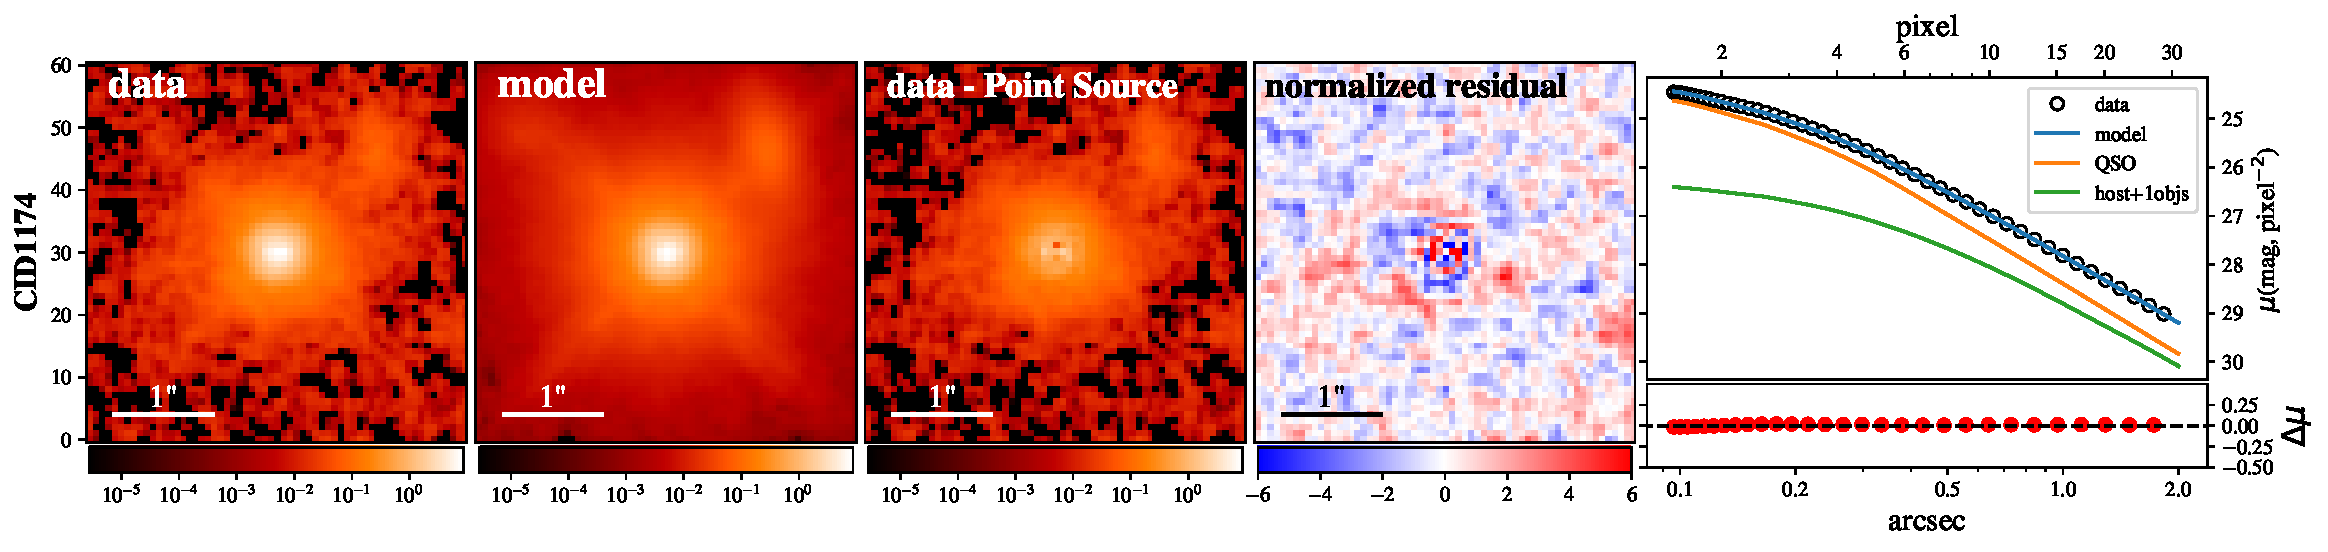
\includegraphics[height=0.25\textwidth]{fig/best_fit_CID1174_SB_profile.pdf}
\caption{\label{fig:AGN_decomp} AGN-host galaxy decomposition of COSMOS-CID1174 based on the \hst/WFC3 F140W image.The panels from left to right are as follows: (1) observed data, (2) best-fit model (AGN+host), (3) data minus the model PSF (i.e., host galaxy free of the AGN), (4) residuals divided by the variance and (5) 1-D surface brightness profiles (top) and the corresponding residual (bottom). The 1-D profiles indicate the surface brightness including the data (open circles), the best-fit model (blue line), the AGN (orange line), and the model for the extended sources (green line, i.e., host and other objects). Note that the 1-D surface brightness profiles are only for illustration purposes. The actual fitting is based on the two-dimensional images. The remaining 31 objects in the sample are shown in Appendix~\ref{sec:restsample}.
}}
\end{figure*} 

\section{AGN-host Decomposition}
\label{sec:analysis}
%Introduce the lenstronomy. Model the PSF in each library.\\
%Inspired by Simon's work, we rank the performance of the each PSF and weight for the final fitting result. 
We simultaneously fit the two-dimensional flux distribution of the central AGN and the underlying host galaxy. Following common practice, we model the central AGN as a scaled point source and the host galaxy as a \sersic\ profile. Note that the actual morphologies of the host galaxies could be more complicated (e.g., bulge+disk). However, the \sersic\ model is an adequate first-order approximation of the surface brightness distribution with a flexible parameterization that provides sufficient freedom to infer the total host flux even for our high redshift sample. We simultaneously fit the nearby galaxies, that happen to be close enough to the AGN, with a \sersic\ model to account for any potential contamination from their extended profiles. The systems CID206 and ECDFS-358 have nearby objects which could not be described by \sersic\ model thus we mask these objects in the fitting procedure.

%Introduce Lenstronomy:
We use the image modeling tool \lenstronomy~\citep{lenstronomy} to perform the decomposition of the host and nuclear light. \lenstronomy\ is a multi-purpose open-source gravitational lens image forward-modeling package written in Python. 
Its flexibility enables us to turn off the lensing channel and focus on the AGN and host decomposition\footnote{As a check, we compared the results from \lenstronomy\ to the commonly used galaxy modeling software {\sc Galfit} and confirm that the results are consistent between the two.}. The main advantage of \lenstronomy\ is that it returns the full posterior distribution of each parameter (i.e., not just the best fit model) and the Laplace approximation of the uncertainties. The input ingredients to \lenstronomy\ include:
\begin{enumerate}
\item AGN imaging data. \\
-- Using aperture photometry, we find that an aperture size with radius $\sim1\farcs{}5$ sufficiently covers the AGN emission of our sample. By default, we extract an image of $61\times61$ pixels (i.e. $4''\times 4''$). If needed, a larger box size would be sufficient to include nearby objects. 
\item Noise level map.\\
-- The origin of the noise in each pixel stems from the read noise, background noise, and Poisson noise from the astronomical sources themselves. We measure these directly from the empty regions of the data. We then calculate the effective exposure time of each pixel based on the drizzled \texttt{WHT} array maps to infer the Poisson noise level. A final noise map includes all of these sources of error. 
  
\item PSF. \\
-- The PSF is directly taken from the PSF library. Usually, a mismatch exists when subtracting the AGN as the scaled PSF, especially at the central parts. While modeling multiply imaged AGN, this mismatch can be mitigated with PSF reconstruction by the iterative method~\citep{Chen2016, Birrer2018}.  However, this approach requires multiple images which are not available in our case.  We remedy this deficiency by using a broad library which should contain sufficient information to cover all the possible PSF. 
\end{enumerate}

%Introduce the final inference using fitting:

The host property of an AGN is determined by the following steps. First, we model the AGN and host using each PSFs in the library. With the input ingredients to \lenstronomy, the posterior distribution of the parameter space is calculated and optimized by adopting the Particle Swarm Optimizer (PSO)\footnote{Note that \lenstronomy\ enables one to further infer the parametric confidence interval using MCMC. In our case, given a fixed PSF, the $1\sigma$ inference of each parameter is extremely narrow. Thus, we only take the best-fit inference using PSO for further calculations. The errors on the fit parameters are assessed by using different PSFs for each object in the sample.}.
To avoid any unphysical results, we set the upper and lower limits on the parameters: effective radius \Reff\ $\in[0\farcs{}1,1\farcs{0}]$, \sersic\ index $n\in[1,7]$.
Then, we rank the performance of each PSF based on the $\chi^2$ value and select the top-eight PSFs as representative of the best-fit PSFs. We determine the host \sersic\ parameters (i.e., flux, \Reff, \sersic\ index) using a weighted arithmetic mean, calculated as follows:

\begin{eqnarray}
\label{eq:weights}
w_i = exp \big(- \alpha \frac{ (\chi_i ^2 - \chi_{best} ^2 )}{2 \chi_{best} ^2} \big),
\end{eqnarray} 
where the $\alpha$ is an inflation parameter so that when $i=8$:
\begin{eqnarray}
\label{eq:alpha}
\alpha \frac{ \chi_{i=8} ^2 - \chi_{best} ^2 }{2 \chi_{best} ^2} = 2,
\end{eqnarray} 
The goal of this recipe is to weight each PSF based on their relative goodness of fit, while ensuring at least eight are used to capture the range of systematic uncertainties. The results do not change significantly if we chose a different number of PSFs, as shown below.

Note that since each AGN was observed in different location of the detector and at a different time, the top-eight PSFs usually vary from one AGN to another. Given the weights, the value of host properties and the root-mean-square ($\sigma$) error are calculated as:
\begin{eqnarray}
\label{eq:infer_value}
\bar{x}  =  \frac{  \sum_{i=1}^{N}   x_i * w_i  }{\Sigma w_i} ,
\end{eqnarray} 
\begin{eqnarray}
\sigma =   \sqrt{ \frac{  \sum_{i=1}^{N}   (x_i -  \bar{x} ) ^2 * w_i  }{\Sigma w_i} },
\end{eqnarray} 
where $N$ is the number of the ranking PSF, i.e., 8.

\noindent In Figure~\ref{fig:AGN_decomp}, we demonstrate the results for COSMOS-CID1174. The adopted weights are listed in Table~\ref{tab:weight_CID1174}. 




%\begin{figure*}
%\centering
%{
%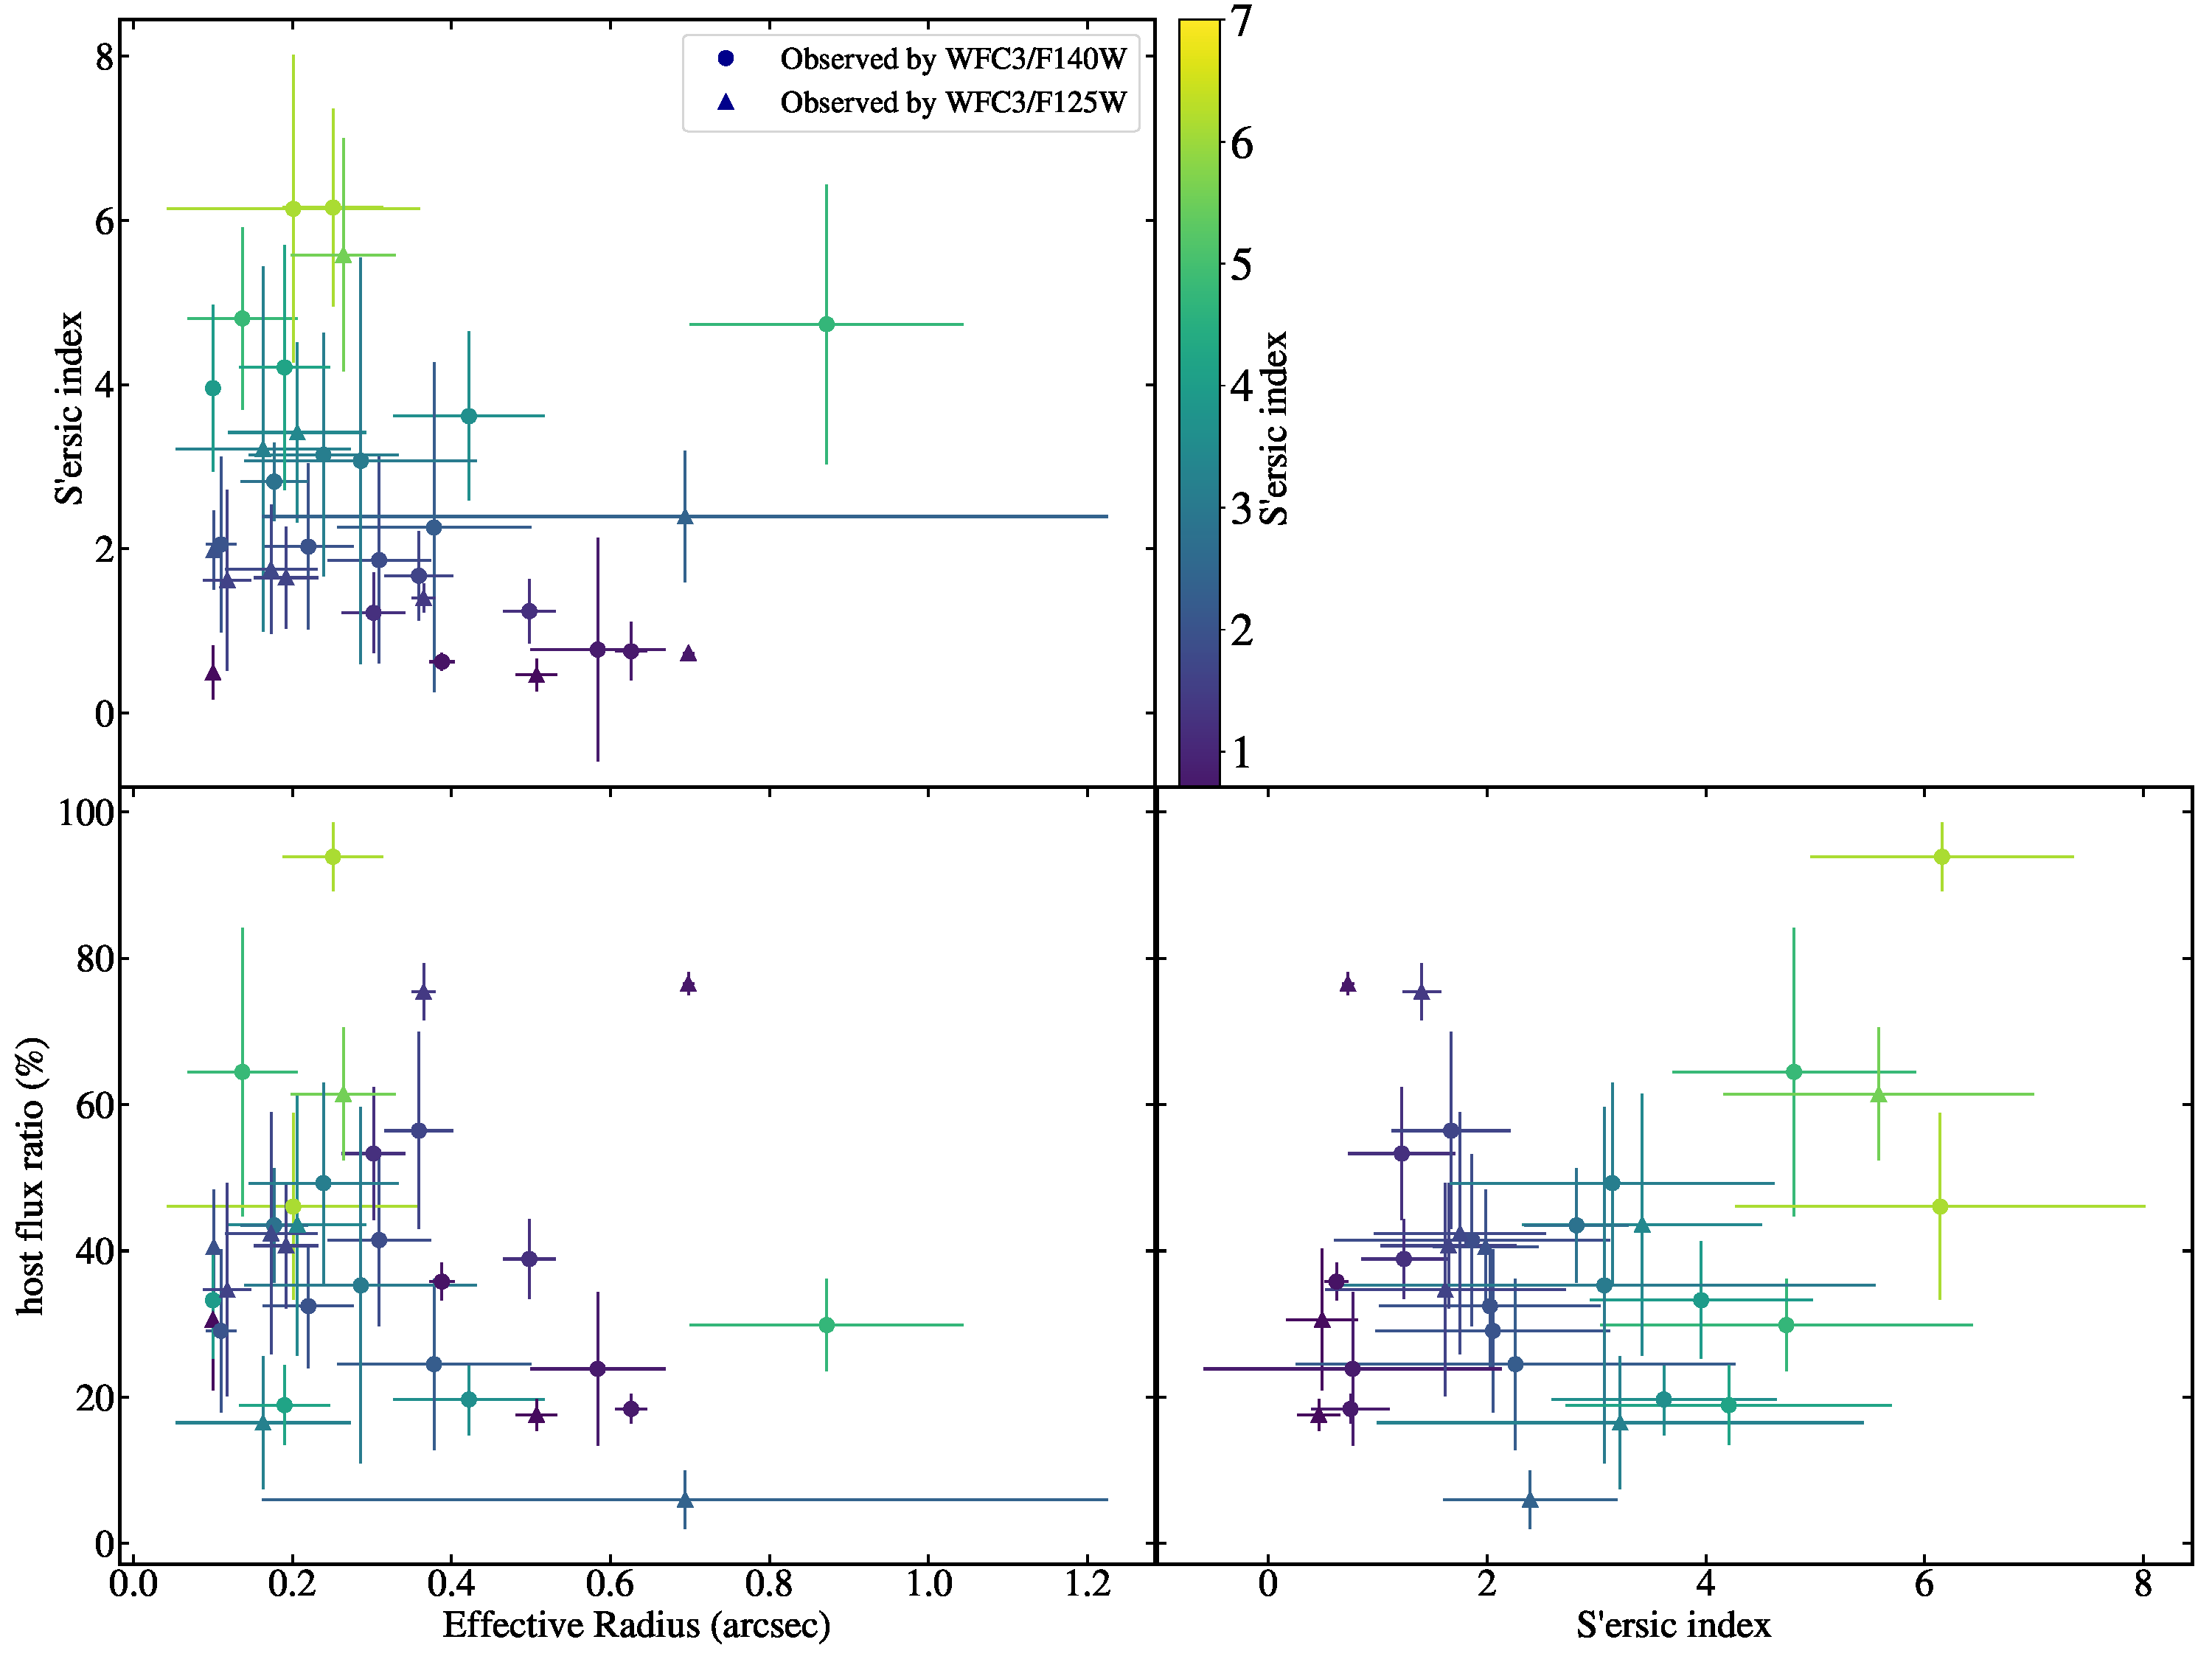
\includegraphics[height=0.5\textwidth]{fig/flux_r_n_corner.pdf}
%}
%\caption{\label{fig:flux_r_n_corner}
%Relations between the measured host galaxy parameters.}
%\end{figure*} 

We apply this approach to all AGNs to determine the global characteristics of the hosts of type-1 AGNs at these high redshifts. We measure the effective radius (\Reff), \sersic\ index and host-to-total flux ratio and describe each of these in the following section. We recognize that these measurements are weighted by the eight top-ranked PSFs. The limited number of top-ranked PSFs may underestimate actual uncertainties. To gauge how the number of top-ranked PSF affects our results, we compare results when also using five and ten top-ranked PSFs. As shown in Figure~\ref{fig:hist_compare}, the results are consistent.

\begin{figure}
\centering
{
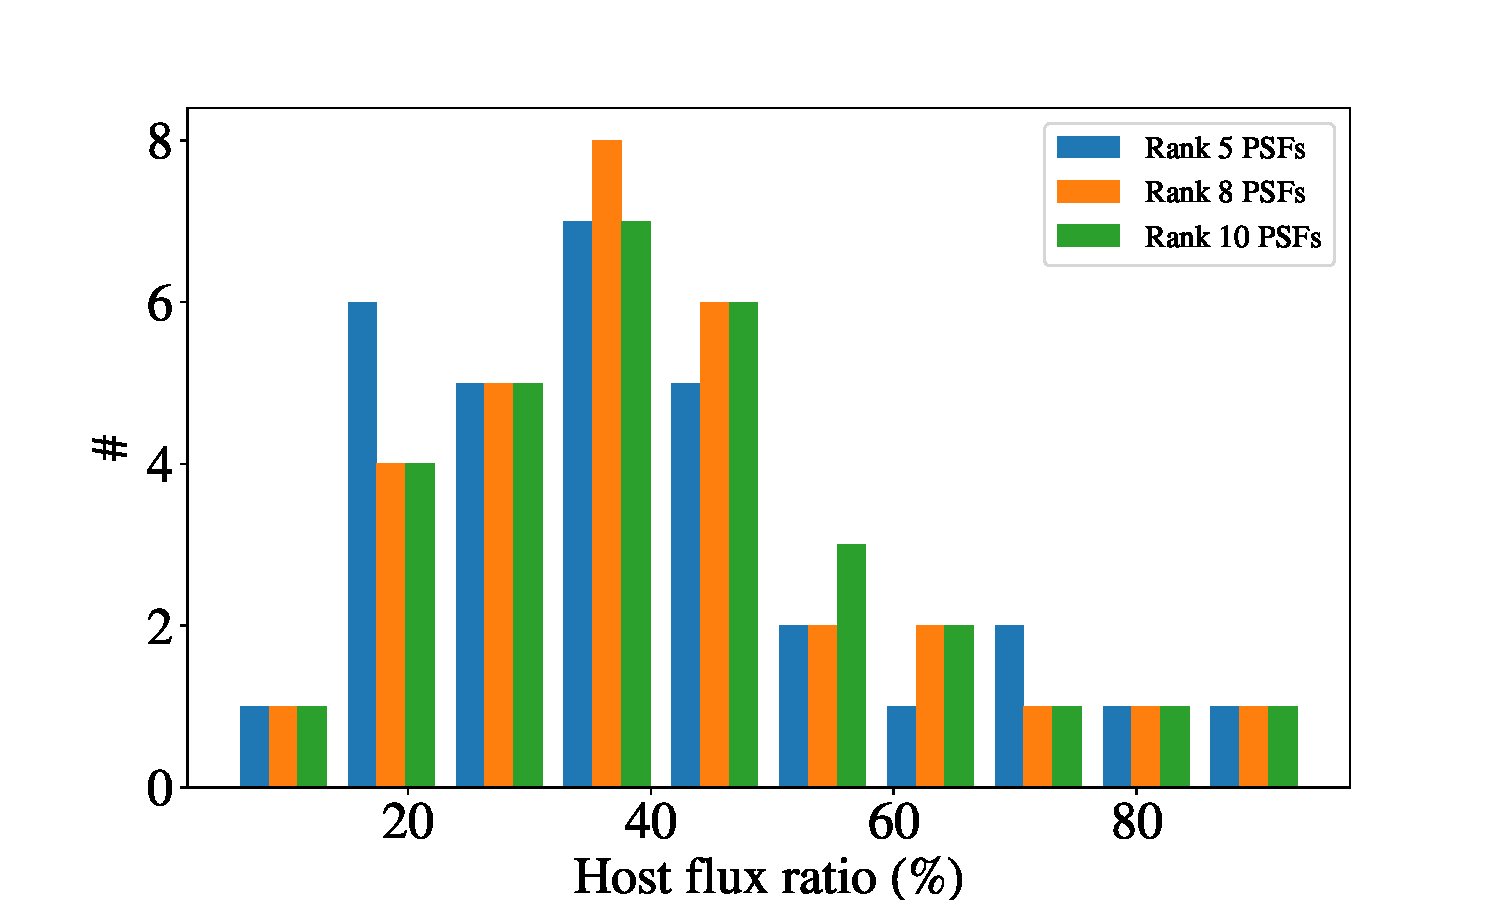
\includegraphics[height=0.25\textwidth]{fig/hist_compare.pdf}
}
\caption{\label{fig:hist_compare} 
Distribution of the host-to-total flux ratio when implementing a different number of top-ranked PSFs.}
\end{figure} 


%The inference of F814w data.
We carry out a similar analysis for 18/32 AGNs in the COSMOS field with ACS/F184W imaging data. We assess their host flux ratio using the same approach as done for the WFC3-IR. The ACS FOV is larger than WFC3 thus we generated 174 PSFs for use. As expected, the detection of the host galaxy in the IR band is of higher significance than the UV due to the effects of dust extinction and the contrast between the (blue) AGN and (red) host. Thus, we fix the \Reff\ and \sersic\ $n$ as the value determined by IR band thus amounting to an assumption that the morphology of the galaxy is consistent between ACS and WFC3 bands. In this case, the only free parameters are the total host and AGN flux. We report the host galaxy properties in Table~\ref{tab:result_sersic}.


\section{Results}
\label{sec:result}

From our AGN-host decomposition, we detect the host galaxy in essentially all cases. \hst/WFC3 images with the AGN component removed are presented in the third panel (i.e., the ``data-point source'' stamps) shown in Figures~\ref{fig:AGN_decomp} and Appendix~\ref{sec:restsample}. While some of the galaxies have nearby neighbors, most are isolated and do not show strong signs of interaction or ongoing mergers. This is relevant for model fitting with smooth \sersic\ profiles and the subsequent determination of the stellar mass. In the following subsections, we described the properties of our ensemble of type-1 AGN host galaxies.
 
\subsection{Host galaxy properties}
\label{sec:result-hosts}
As shown in Figure~\ref{fig:hist_compare}, the host-to-total flux ratio of the sample spans a wide range from 10\% to 90\% with most of the sample concentrated between 20\% to 50\%. Those with flux ratios above $\sim20\%$ have a higher degree of significance with respect to the detection of the host galaxy, while the very few cases around 10\% should be considered as marginal detections. 

The distributions of effective radius \Reff\ and \sersic\ index are shown in Figure~\ref{fig:hist_rn}. These values are distributed within the allowed range and not concentrated on either the upper or lower bound. The \Reff\ of our sample are between $\sim$1-7~kpc (peaked at $\sim$2.2~kpc). Nearly half (15/32) of our systems have \sersic\ index $n<2$, indicating they have a significant disk component, likely in addition to the presence of a bulge. Five systems had a high \sersic\ index ($n>4.5$) for the first run; we use $n\in[1,4]$ as prior to re-fit these systems and find that the changes on the inference of their host luminosity are very limited ($<0.03$ dex).

We compare the morphology of AGNs host galaxies to the inactive ones from the CANDELS/COSMOS imaging survey. We identify 4401 inactive galaxies in a comparable redshift range ($1.2<z<1.7$) whose \sersic\ properties are inferred by \citet{VDwel++2012} using \galfit, and their stellar masses are derived based on 3-D-\hst\ spectroscopic survey~\citep{Momcheva2016, Brammer2012}. We compare the histogram of the inferred \Reff\ and \sersic\ index to the inactive galaxies in Figure~\ref{fig:hist_rn}, where we find no significant difference between their distributions and median value. We also test whether the distributions can be drawn from the same parent population using a Kolmogorov-Smirnov test and determining the p-value to be 0.42 and 0.04 for \Reff\ and $n$, respectively. We conclude that the host galaxies of our AGN sample are representative of the overall population of galaxies, with a significant disk component, at comparable luminosity and stellar mass at the same redshift. In Section~\ref{sec:bh_bulge}, we use this information to infer the likely bulge masses, hence the \mbh\ -- \bmass\ relation.




%In Figure~\ref{fig:Mstar-rn}, we plot the \smass\ versus the \Reff\ and \sersic\ index. The color coding is based on the filter flux ratio between WFC3 and ACS. The distribution of \smass-\Reff\ relation show that our AGN hosts concentrate at the high end of the stellar mass, close to the red sequence. 
%\begin{figure*}
%\centering
%\begin{tabular}{c c}
% \hspace{-2.5em}
%{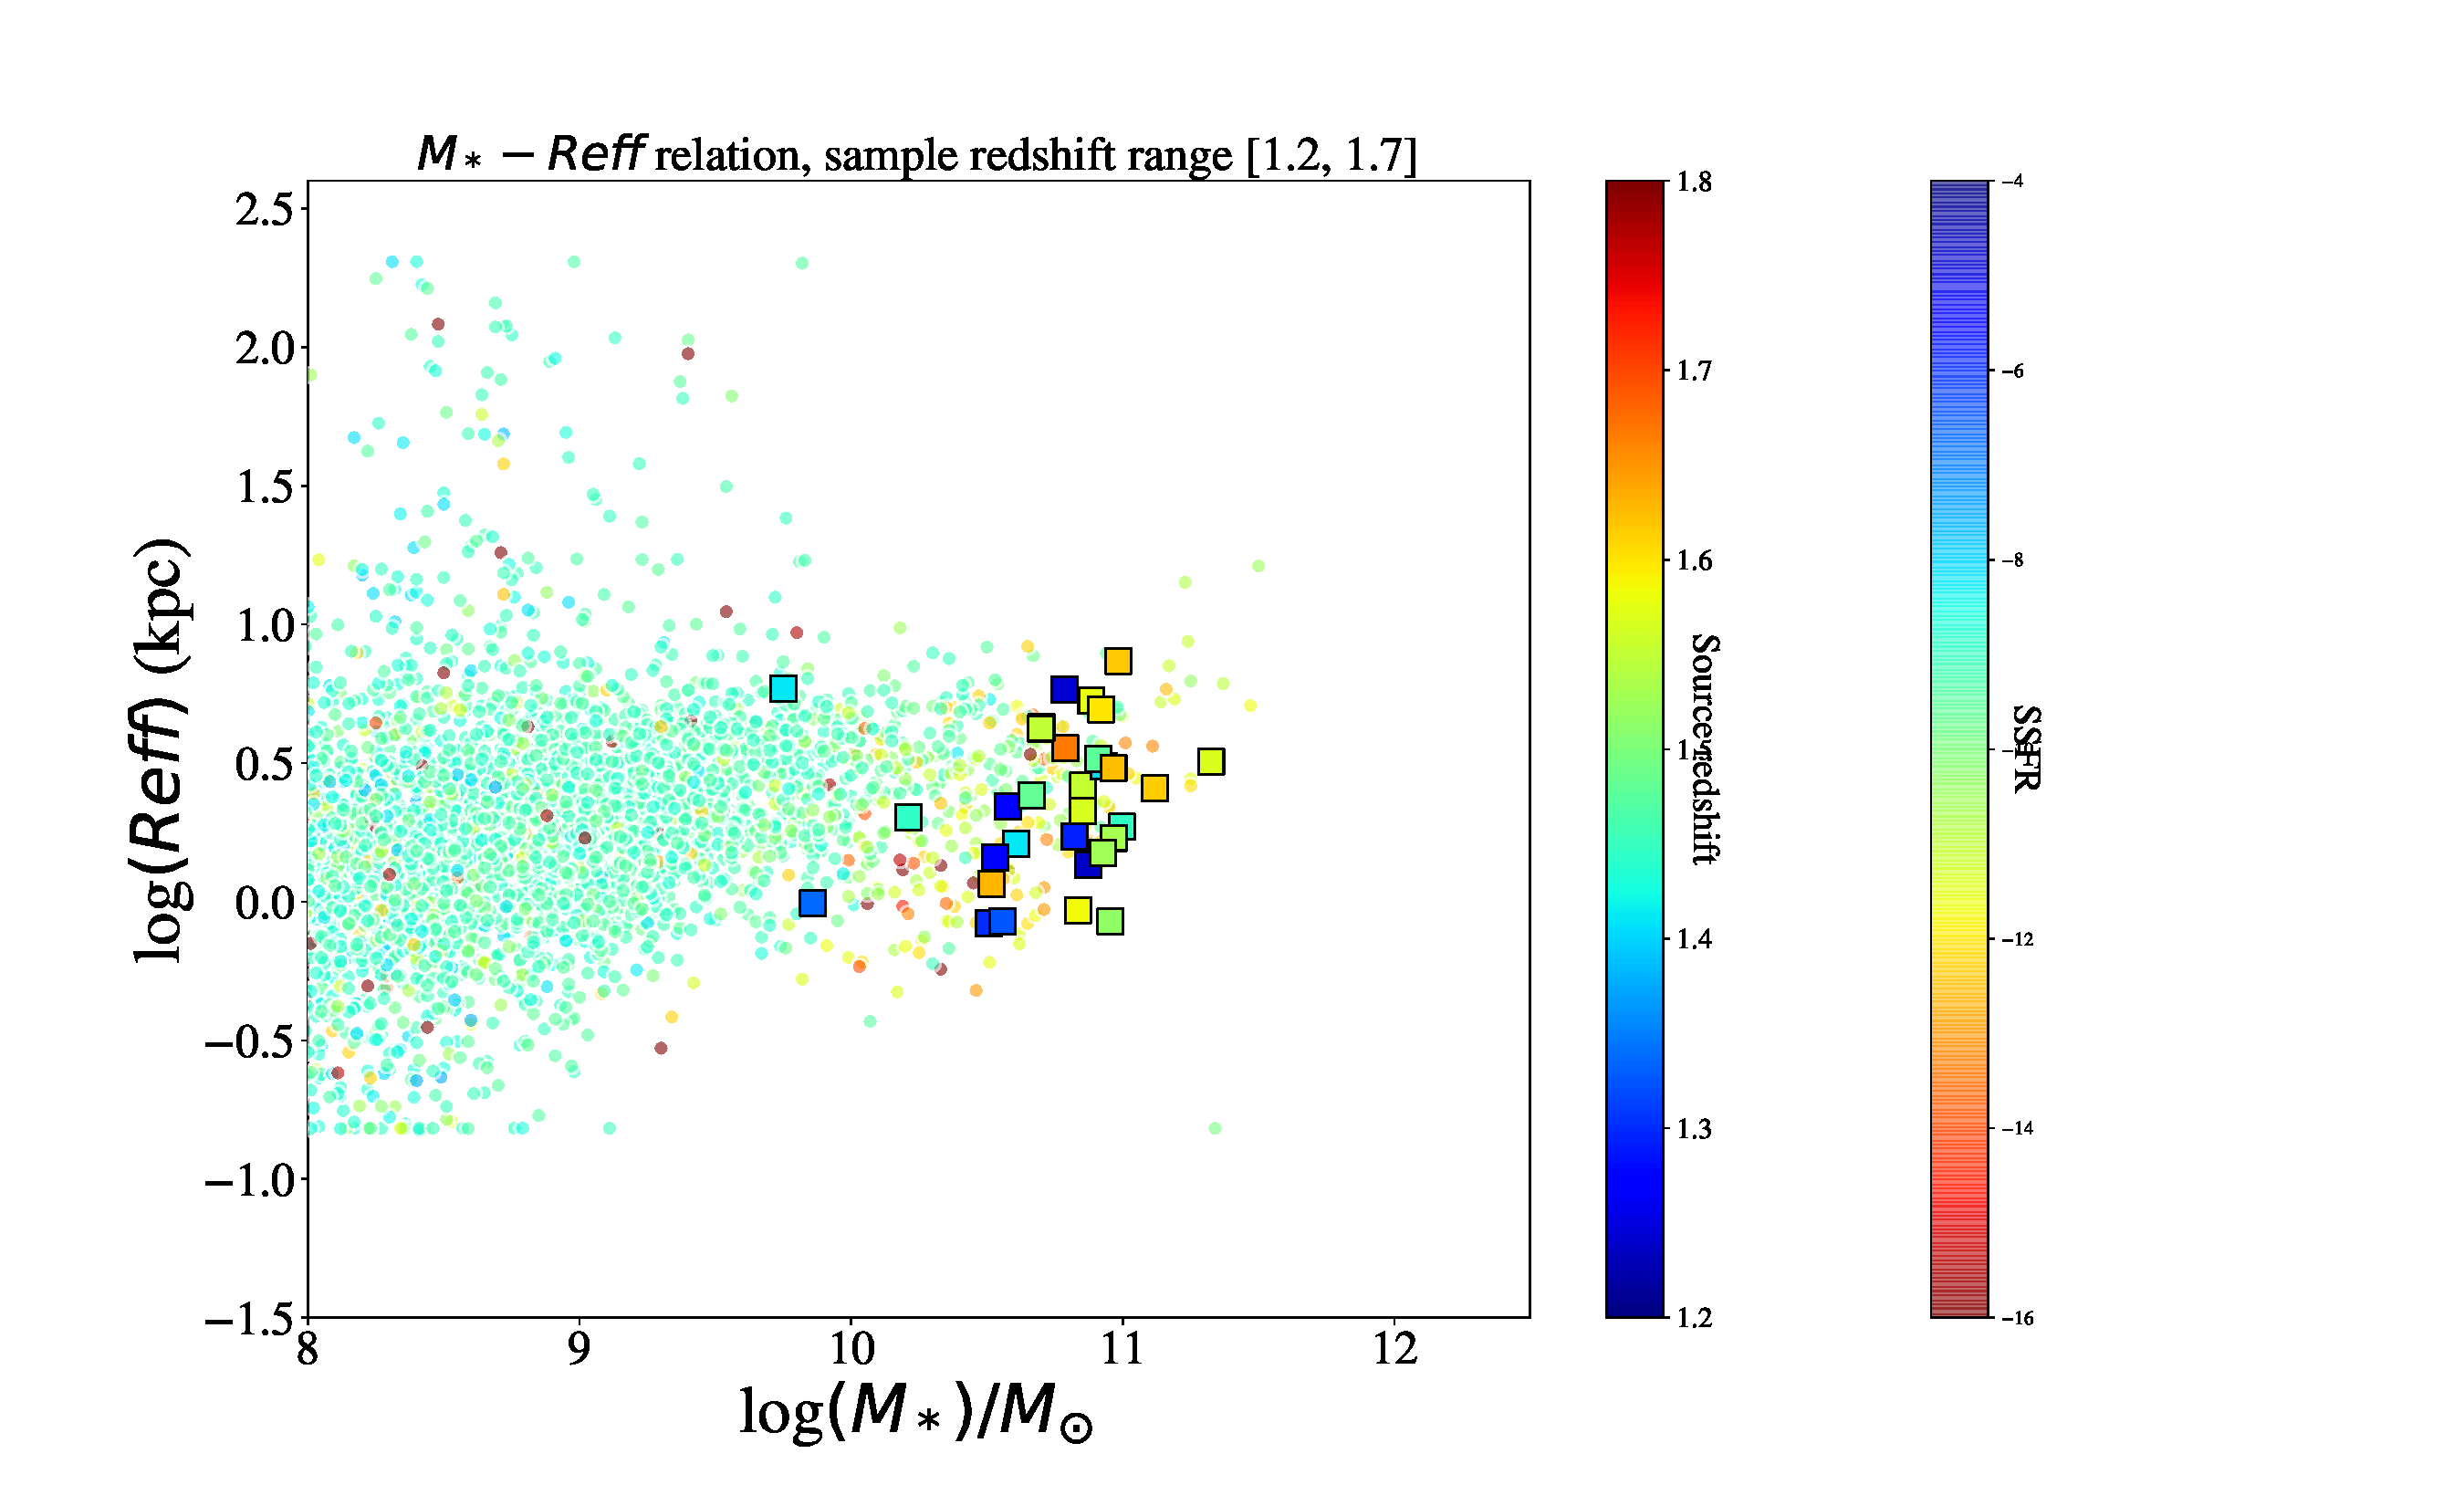
\includegraphics[trim = 0mm 0mm 90mm 0mm, clip, height=0.45\textwidth]{fig/Mstar-Reff.pdf}}&
%{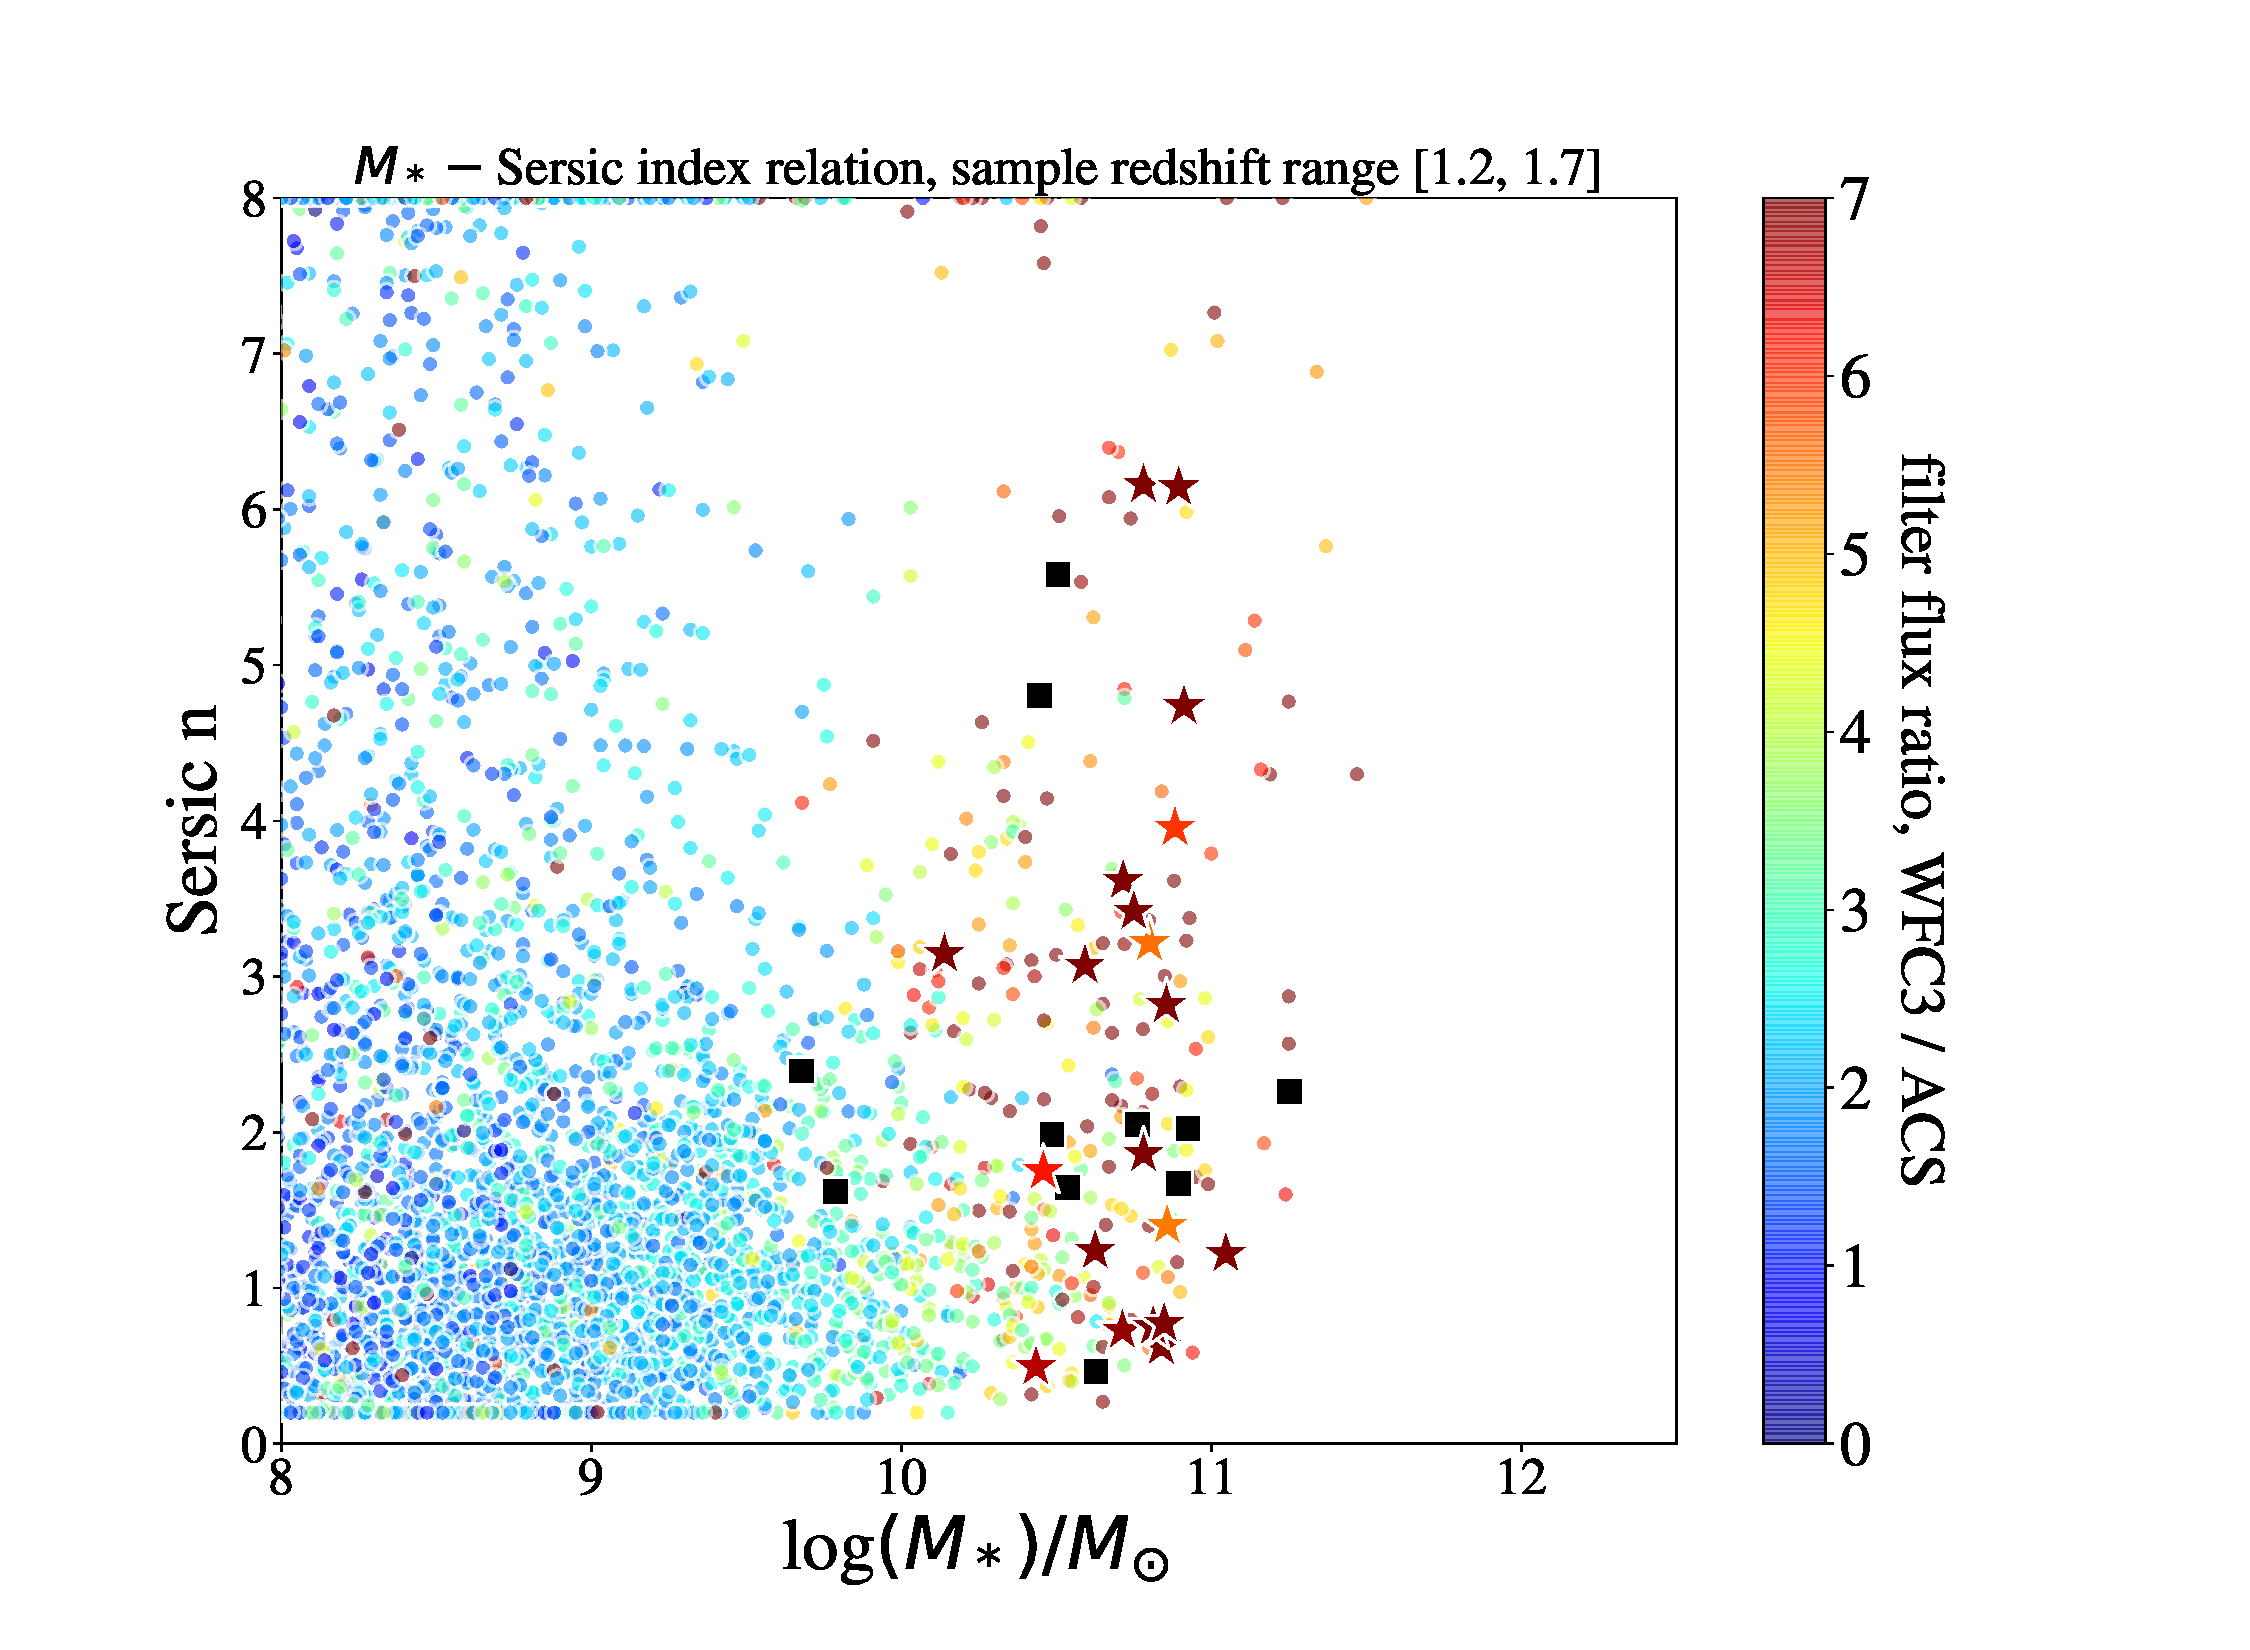
\includegraphics[ height=0.45\textwidth]{fig/Mstar-Sn.pdf}}\\
%\end{tabular}
%\caption{\label{fig:Mstar-rn} 
%The comparison of the galaxy properties between our 32 AGNs' hosts to the CANDELS sample including 4401 inactive galaxies (circles). The color coding is based on the filter flux ratio between WFC3 and ACS. For CANDELS sample, the WFC3/F125W flux is taken. The black squares are the AGN samples with only WFC3 band observation.
%}
%\end{figure*} 

\begin{figure}[ht]
%\centering
%\begin{tabular}{c c}
%{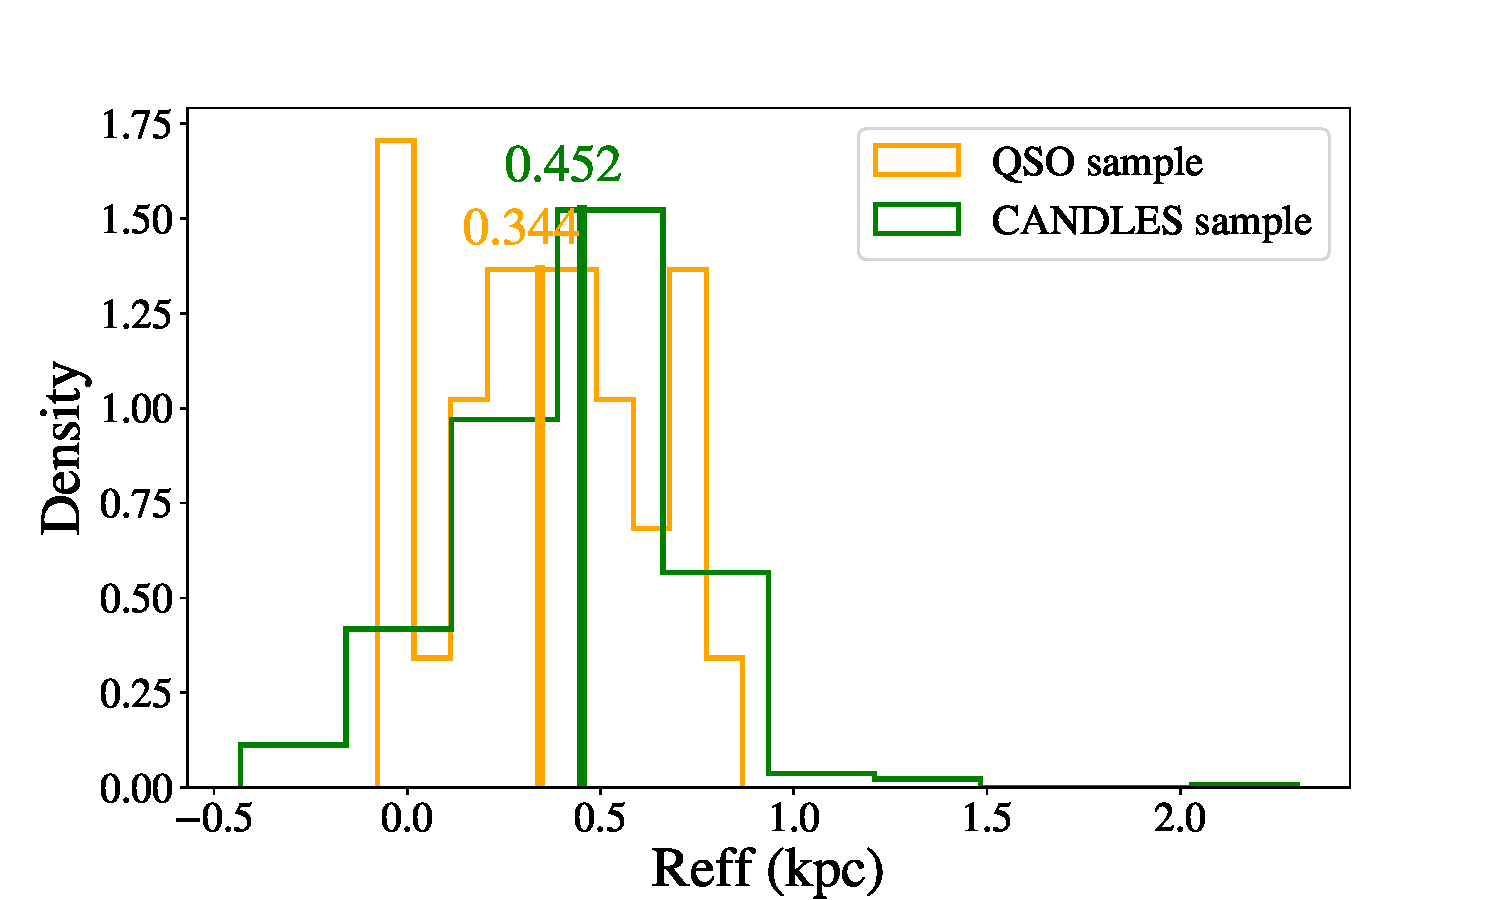
\includegraphics[ height=0.3\textwidth]{fig/Hist_Reff.pdf}}&
%{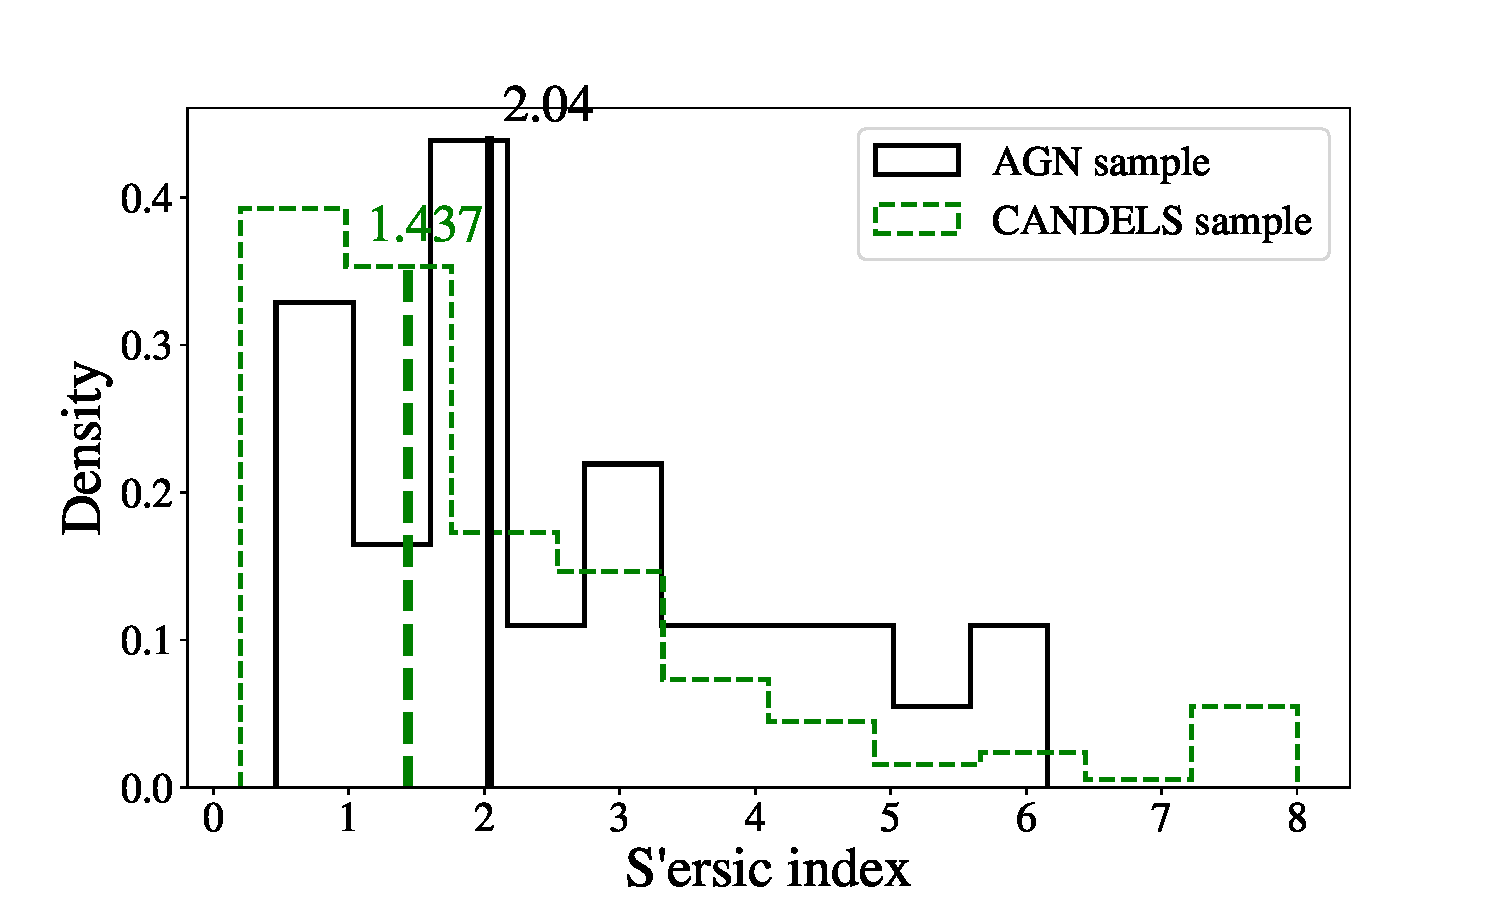
\includegraphics[ height=0.3\textwidth]{fig/Hist_Sn.pdf}}
%\end{tabular}
\epsscale{1.2}
\plotone{fig/Hist_Reff.pdf}
\plotone{fig/Hist_Sn.pdf}
\caption{\label{fig:hist_rn} 
The comparison of the histogram of the \Reff\ (top panel) and \sersic\ $n_s$ (bottom panel), with median value indicated. For comparison, we show the distribution of CANDELS galaxies at similar redshifts and stellar masses to our type-1 AGN sample.}
\end{figure} 
%



%We also comparing the distribution of the \sersic\ values to the inactive galaxies in the Appendix~\ref{sec:comp_inactive} and find that our high-$z$ AGN host have very similar distribution. %Thus, we assume the inactive galaxies and our AGN hosts have similar bulge-total ratio so that we can infer the bulge stellar mass of our sample, as shown below.

\subsection{Rest-frame colors}

For 18/32 AGNs, we have multi-band host magnitudes that enable us to select an appropriate stellar population template to determine rest-frame luminosities and stellar masses for the overall sample. To minimize the uncertainty associated with these corrections, we use this template to interpolate to the rest-frame R band which is very close to the observed wavelengths.  We find that a 1~Gyr stellar population with solar metallicity and a Chabrier IMF~\citep{Bruzual2003} provides a good match to the observed colors of our sample (see Figure~\ref{fig:compare_temp}). We note that the choice is not unique, and other combinations of ages and metallicities and star formation history could match the observed colors and would provide very similar R-band magnitudes, and also stellar masses \citep{Bell2000, Bell2001}. %(cite Bell \& de Jong 2001, 2003),

\begin{figure}
\centering
{\includegraphics[width=0.4\textwidth]{fig/comp_gtemp_1Gyrs.pdf}}
\caption{\label{fig:compare_temp} 
Comparison of the inferred rest-frame R band magnitude based on the adopted stellar population, using 18/32 AGNs which have both WFC3 and ACS imaging data.
}
\end{figure} 
 
\subsection{\mbh-\lhost\ relation}\label{sec:ml}

Adopting the 1~Gyr stellar population, we perform a K-correction to derive the rest-frame R-band magnitude of our sample. As mentioned above, since the WFC3 filter is already close to the rest-frame R-band, we expect the $M_R$ uncertainty introduced by this K-correction to be within 0.05~mag. We derive the rest-frame R band luminosity from $\log L_R/L_{R, \odot} = 0.4\times(M_{R, \odot}-M_R)$, where $M_{R, \odot}=4.61$~\citep{Blanton07}. $L_R$ ranges between $\log L_R \in [9.5, 11.5]$ ($L_{\odot,R}$) with individual values listed in Table~\ref{tab:result_sersic}. 

We show the relation between \mbh\ and \lhost\ in Figure~\ref{fig:ML} with comparison samples. For reference, we fit the local data with a linear relation,

\begin{eqnarray}
\label{eq:MLlocal}
\log \big( \frac{\mathcal M_{\rm BH}}{10^{7}M_{\odot}})= \alpha + \beta \log(\frac{L_R}{10^{10}L_{\odot}}),
\end {eqnarray}

\noindent which enables a direct comparison between our high-$z$ sample and the local relation. The distribution of our data appears to be in good agreement with the local relation and the other AGN samples at lower redshift. Therefore, the observational data indicate that the relation between black hole mass and the host luminosity are similar at different period of the universe. In Appendix~\ref{sec:ml-ev}, we explore how the high-$z$  sample would evolve in this plane solely with luminosity evolution of the host galaxy as done in past studies \citep[e.g., ][]{Ding2017b}. 

We note that there are outliers that deviate from the distribution of overall sample, such as SXDS-X763. We suspect that this source may have abnormal host properties. Indeed, the value of \Reff\ has a large uncertainty ($\sim 75\%$) and the host-to-total flux ratio is the lowest of the high-$z$ sample ($<10\%$). 

%Considering that both the black hole and host galaxy are expected to evolve over cosmic time, it is essential to transfer high-$z$ measurements to their values at today so as to compare them in an equivalent frame. We will make this comparison taking the evolution effect into account in Section~\ref{sec:ml-ev}.



%For CDFS-1 and CDFS-724, their host are \Reff$<0\farcs{}15$, smaller than the PSF FWHM. Moreover, the broad emission line of \mbh\ are from \citet{Suh2015} which could have systemic to \citet{Schulze2018}. Thus, the measurements of these three systems have less fidelity. 

\begin{figure}
\centering
{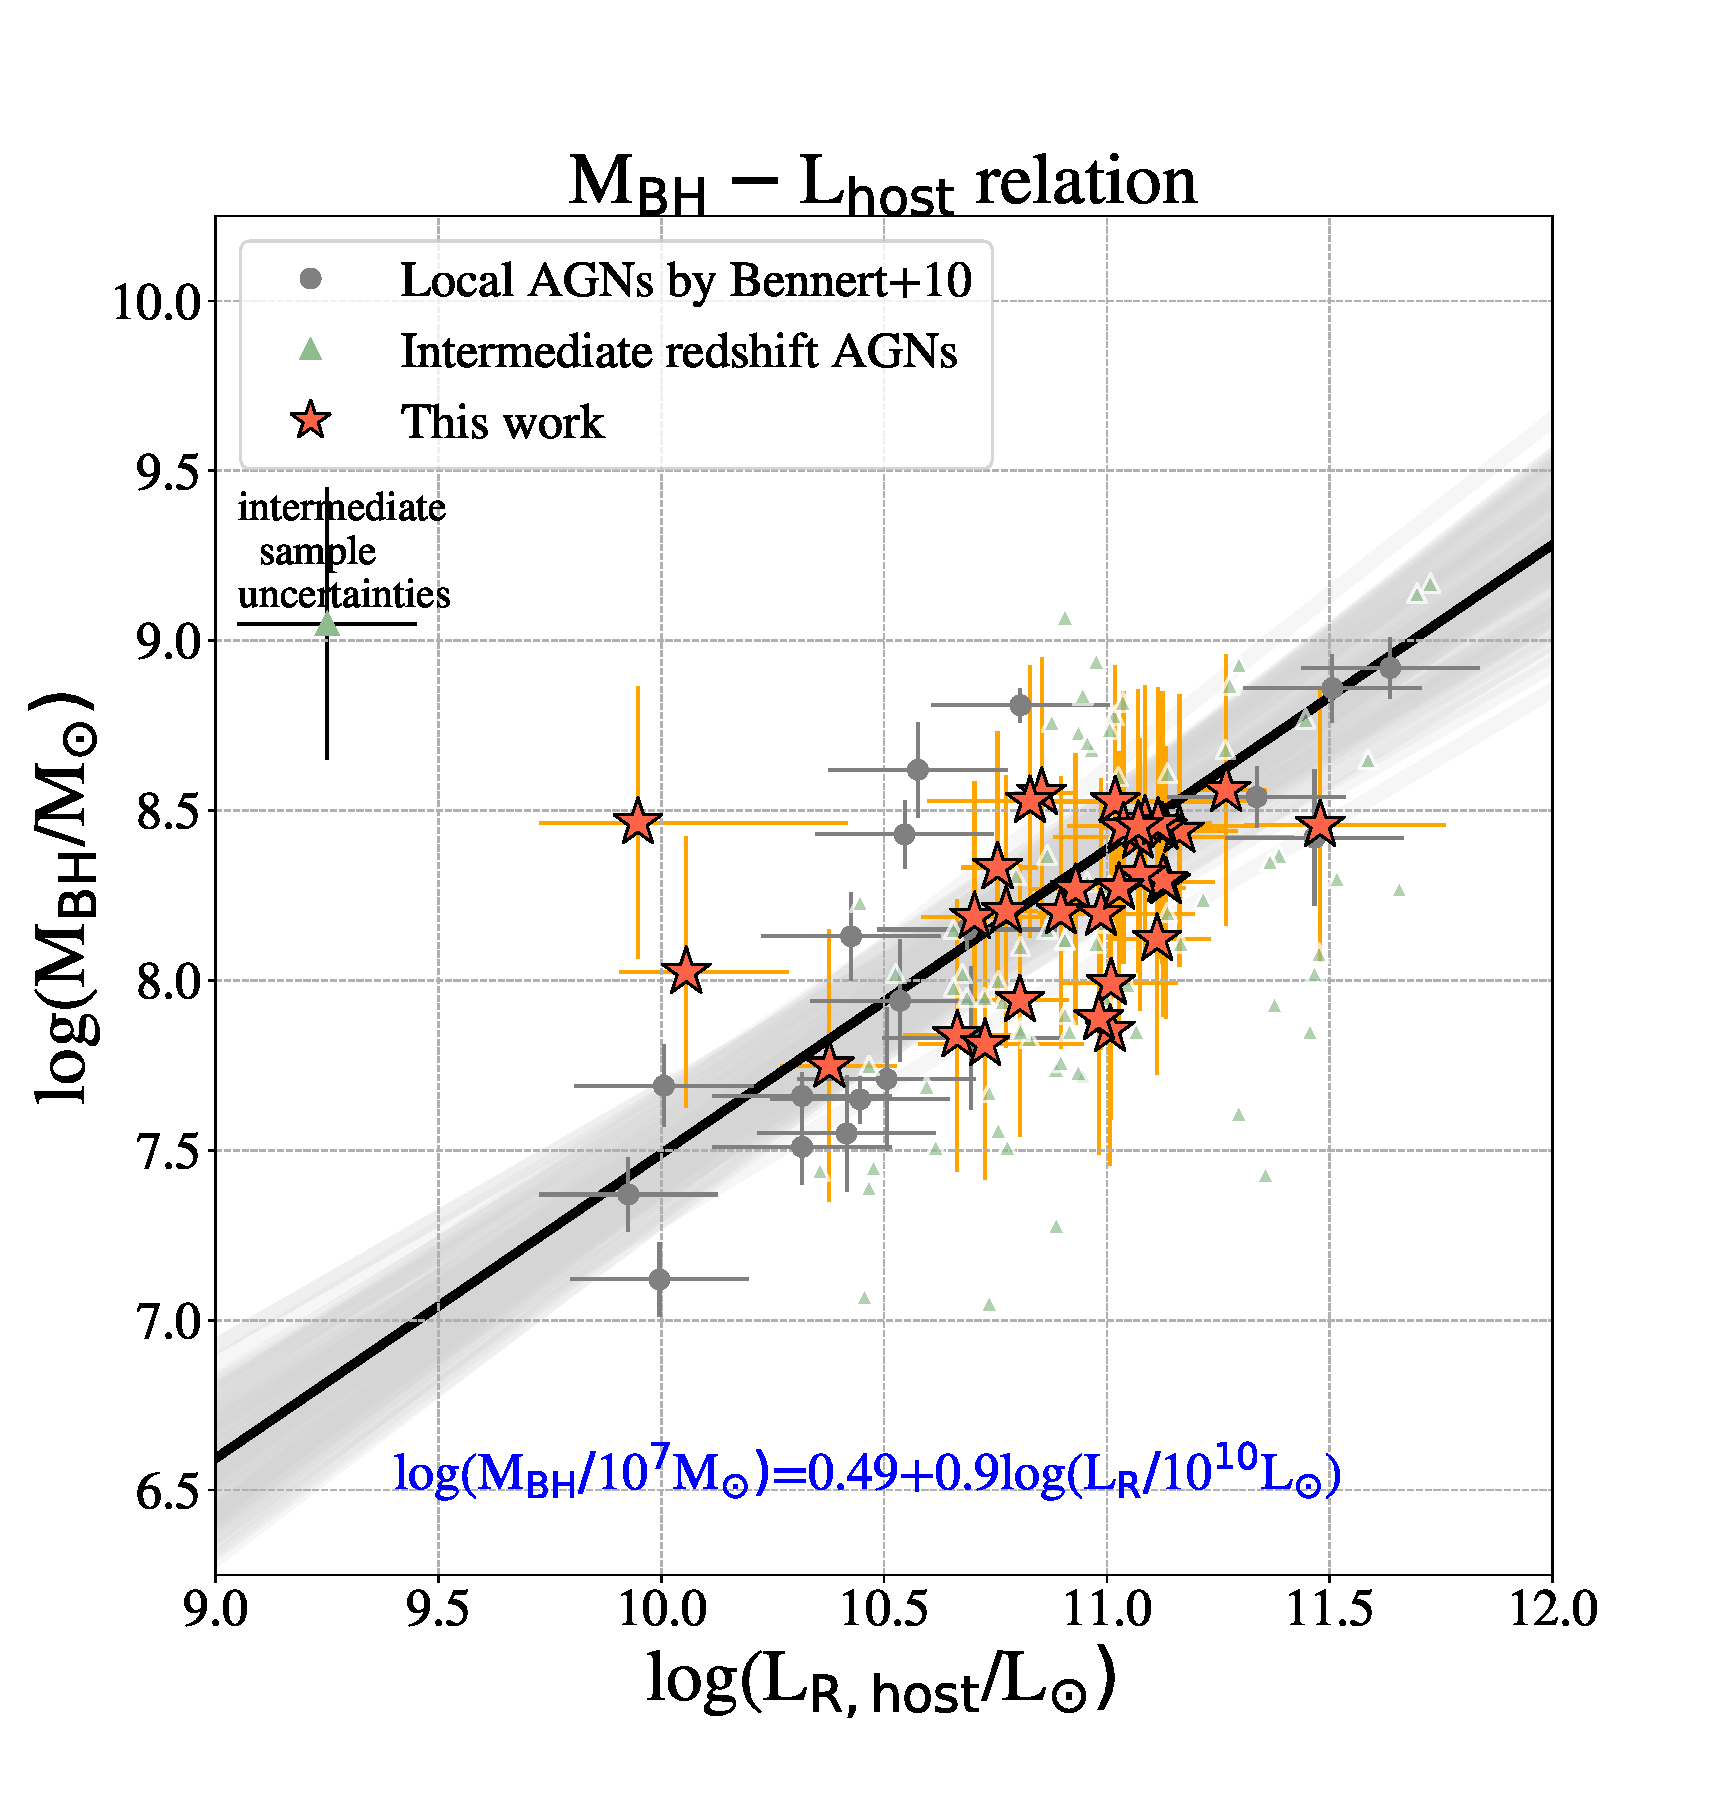
\includegraphics[width=0.5\textwidth]{fig/MBH-L_obs.pdf}}
\caption{\label{fig:ML} 
Black hole mass vs. R-band luminosity relation. The black line and the blue colored equation indicates the best-fit result of local sample as given in Equation~\ref{eq:MLlocal}, with $1-\sigma$ confidence interval indicated by gray region.
}
\end{figure} 

\subsection{\mbh-\smass\ relation}\label{sec:mm}

To fulfill our purpose of acquiring the NIR imaging with \hst, we use the host luminosity along with color information to estimate the stellar mass content of each host galaxy  based on the mass-to-light ratio of the adopted stellar population. The uncertainty level associated with the stellar mass is expected to be of order 0.1~dex (changing the IMF would effect all our stellar masses systematically). We find $M_*$ ranges between $\log M_* \in [9.7, 11.3]$ ($M_{\odot}$). These values are listed in Table~\ref{tab:result_sersic}. 

In Figure~\ref{fig:MM}, we plot the our \mbh -- \smass\ measurements and find that the distributions in this plane for the four samples are similar. However, there is a slight shift of the high-$z$ data towards higher black hole masses at a fixed host mass. In Figure~\ref{fig:MM-vz}, we plot, as a function of redshift, the mass ratio ($right$ panel) and the mass ratio difference ($\Delta \log \mathcal M_{\rm BH} = \log \big( \frac{\mathcal M_{\rm  BH}}{10^{7}M_{\odot}}) -\alpha-\beta\log(\frac{M_*}{10^{10}M_{\odot}})$ which is considered as the difference between the high redshift data and the best-fit local relation; $left$ panel). For our high-$z$ sample, we find the average $\Delta \log \mathcal M_{\rm BH}$ to be 0.3, a factor of two higher than the local mass ratio as indicated by the top green circle in Figure~\ref{fig:MM-vz}.

As with Equation~\ref{eq:MLlocal}, we fit the \mbh-\smass\ data with a linear relation as:
\begin{eqnarray}
\label{eq:MMlocal}
\log \big( \frac{\mathcal M_{\rm BH}}{10^{7}M_{\odot}})= \alpha + \beta \log(\frac{M_*}{10^{10}M_{\odot}}),
\end {eqnarray}

\noindent and an evolution term parameterized in the following form:

\begin{eqnarray}
\label{eq:offset}
\Delta \log \mathcal M_{\rm BH}= \gamma \log (1 + z).
\end{eqnarray} 

If perform such a fit based on the {\it observed} data (i.e., no correction for selection effects), we obtain $\gamma  = 0.78 \pm 0.26$ that may be tentatively considered as evidence for evolution. Even with the exclusion of the few outliers, there is an evolution in the relation with $\gamma  = 0.65 \pm 0.27$. The best-fit {\it observed} evolution model is shown in Figure~\ref{fig:MM-vz}.

\begin{figure}
\centering
{
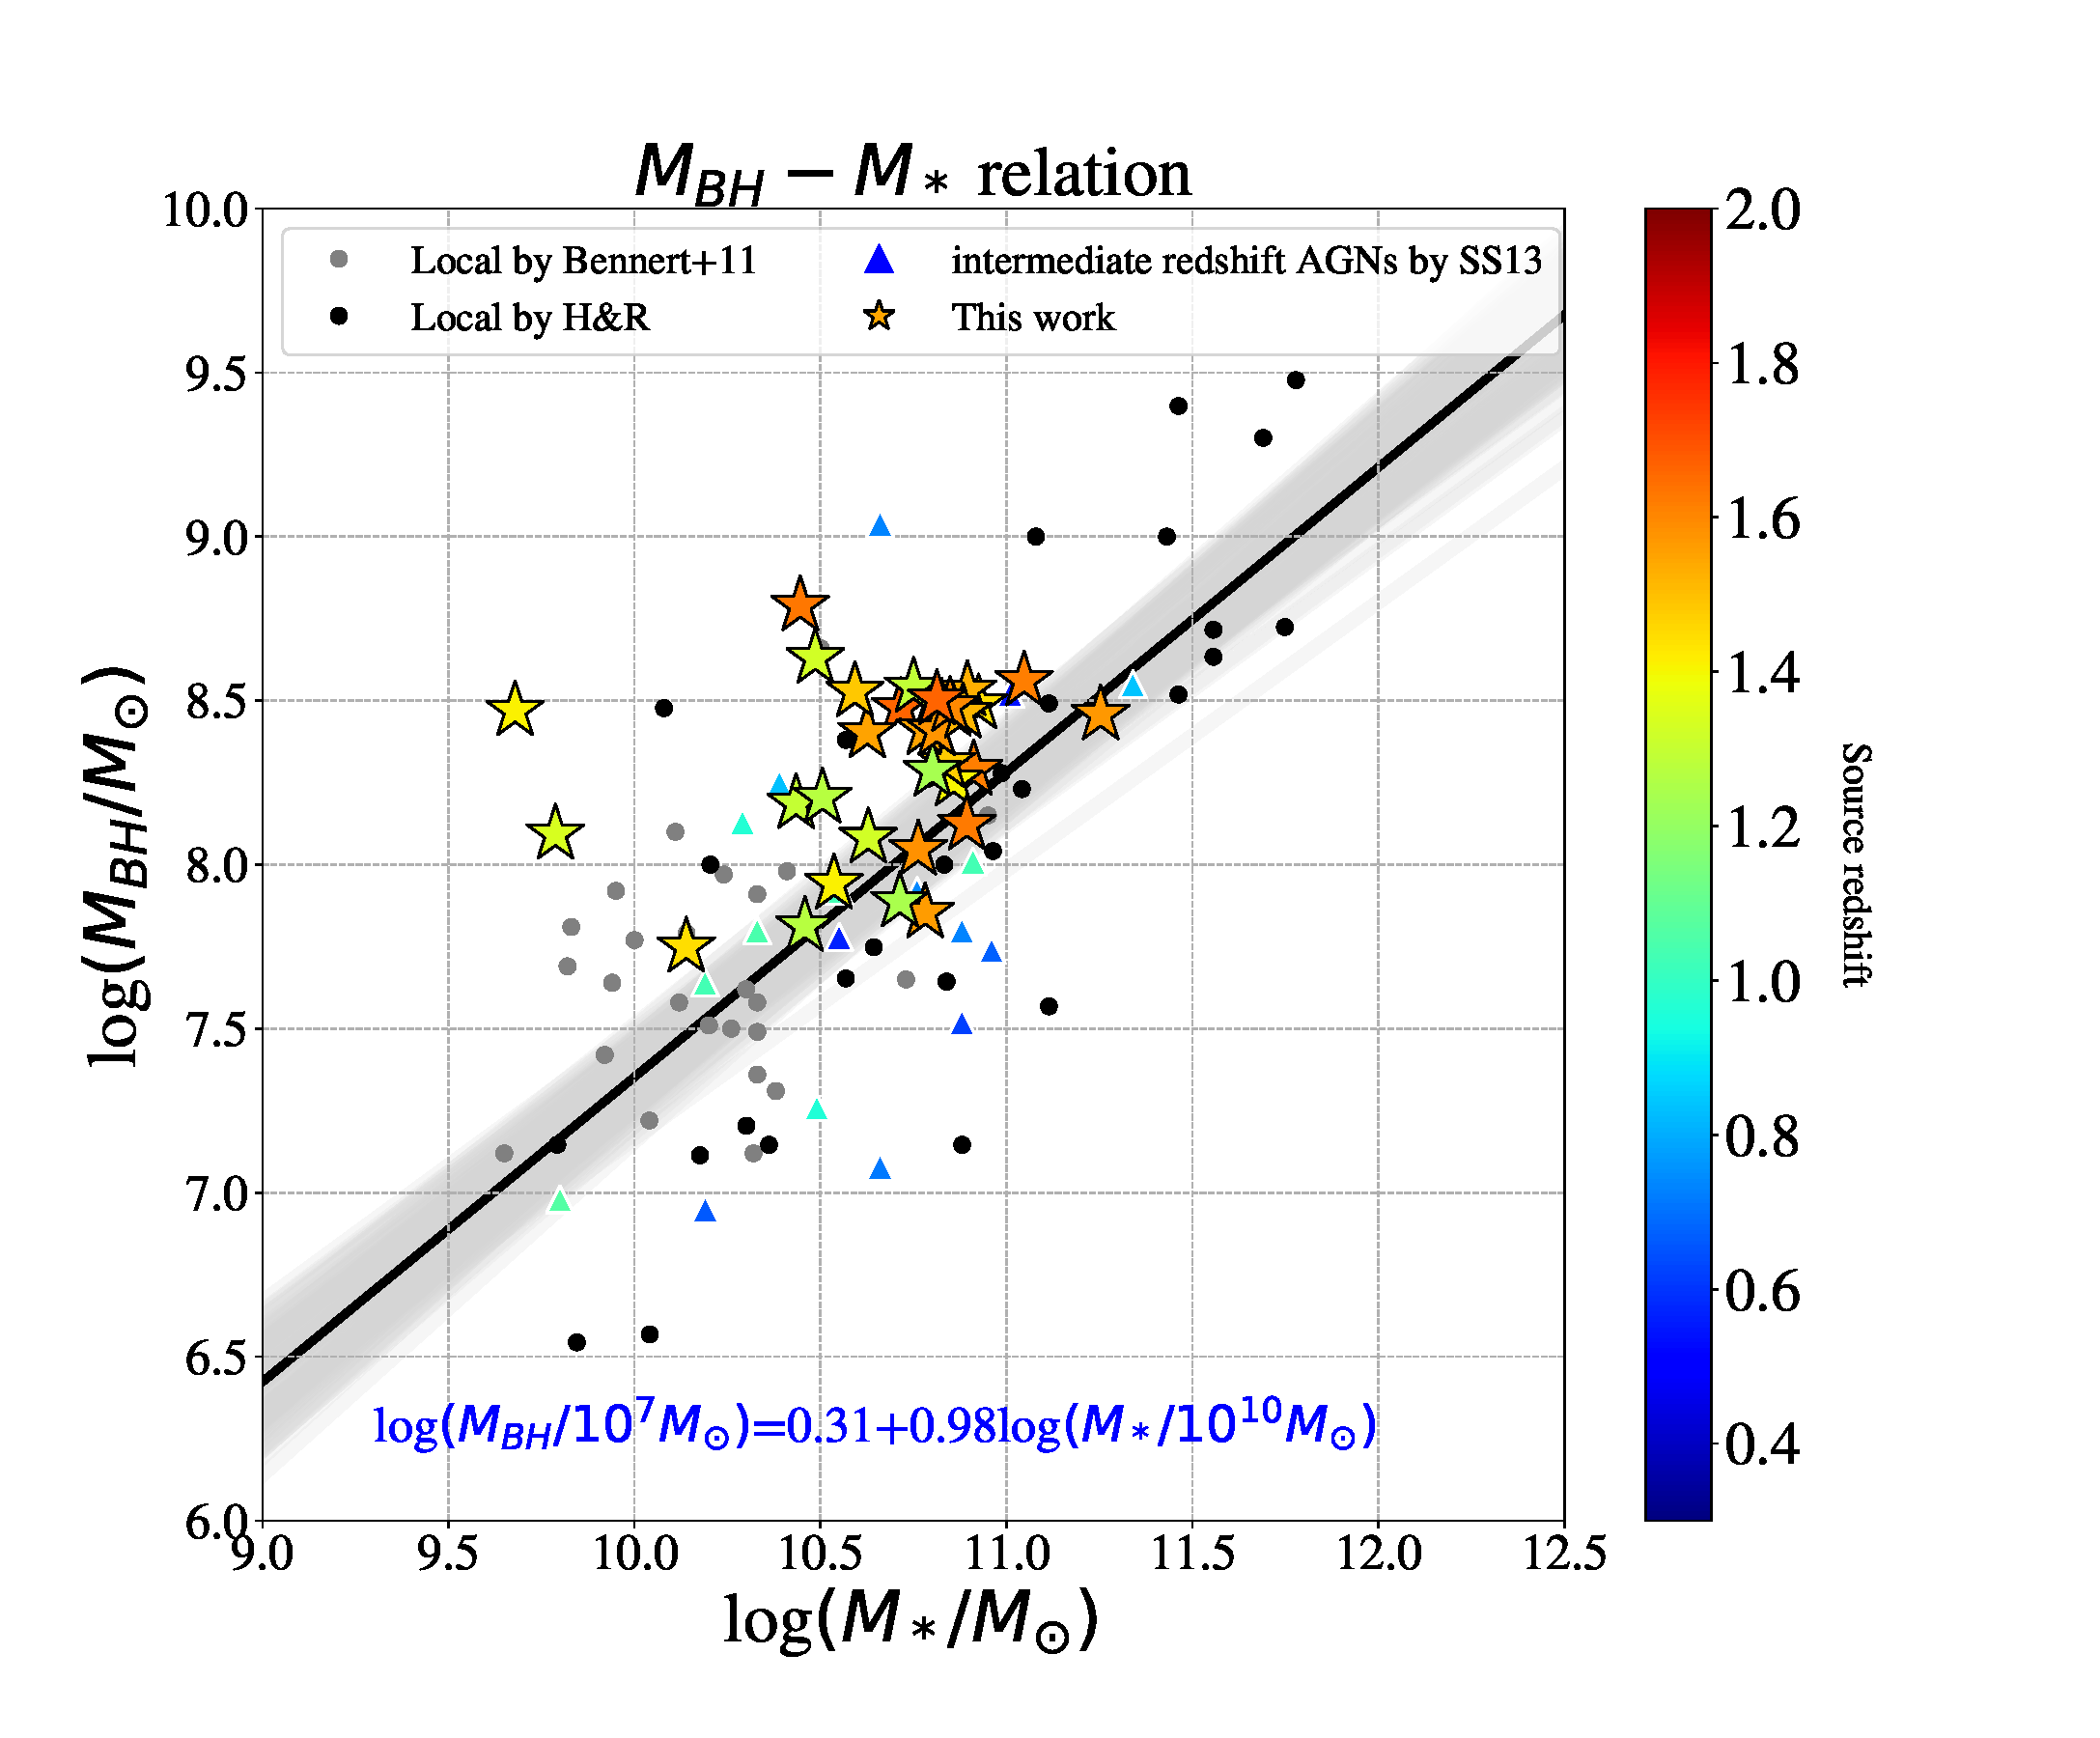
\includegraphics[width=0.5\textwidth]{fig/MBH-Mstar.pdf}
}
\caption{\label{fig:MM} 
Black hole mass vs. stellar mass relation ( \mbh -- \smass\ ). The best-fit local relation is shown as described in Fig.~\ref{eq:MLlocal}.
}
\end{figure} 

\begin{figure*}
\centering
\begin{tabular}{c c}
{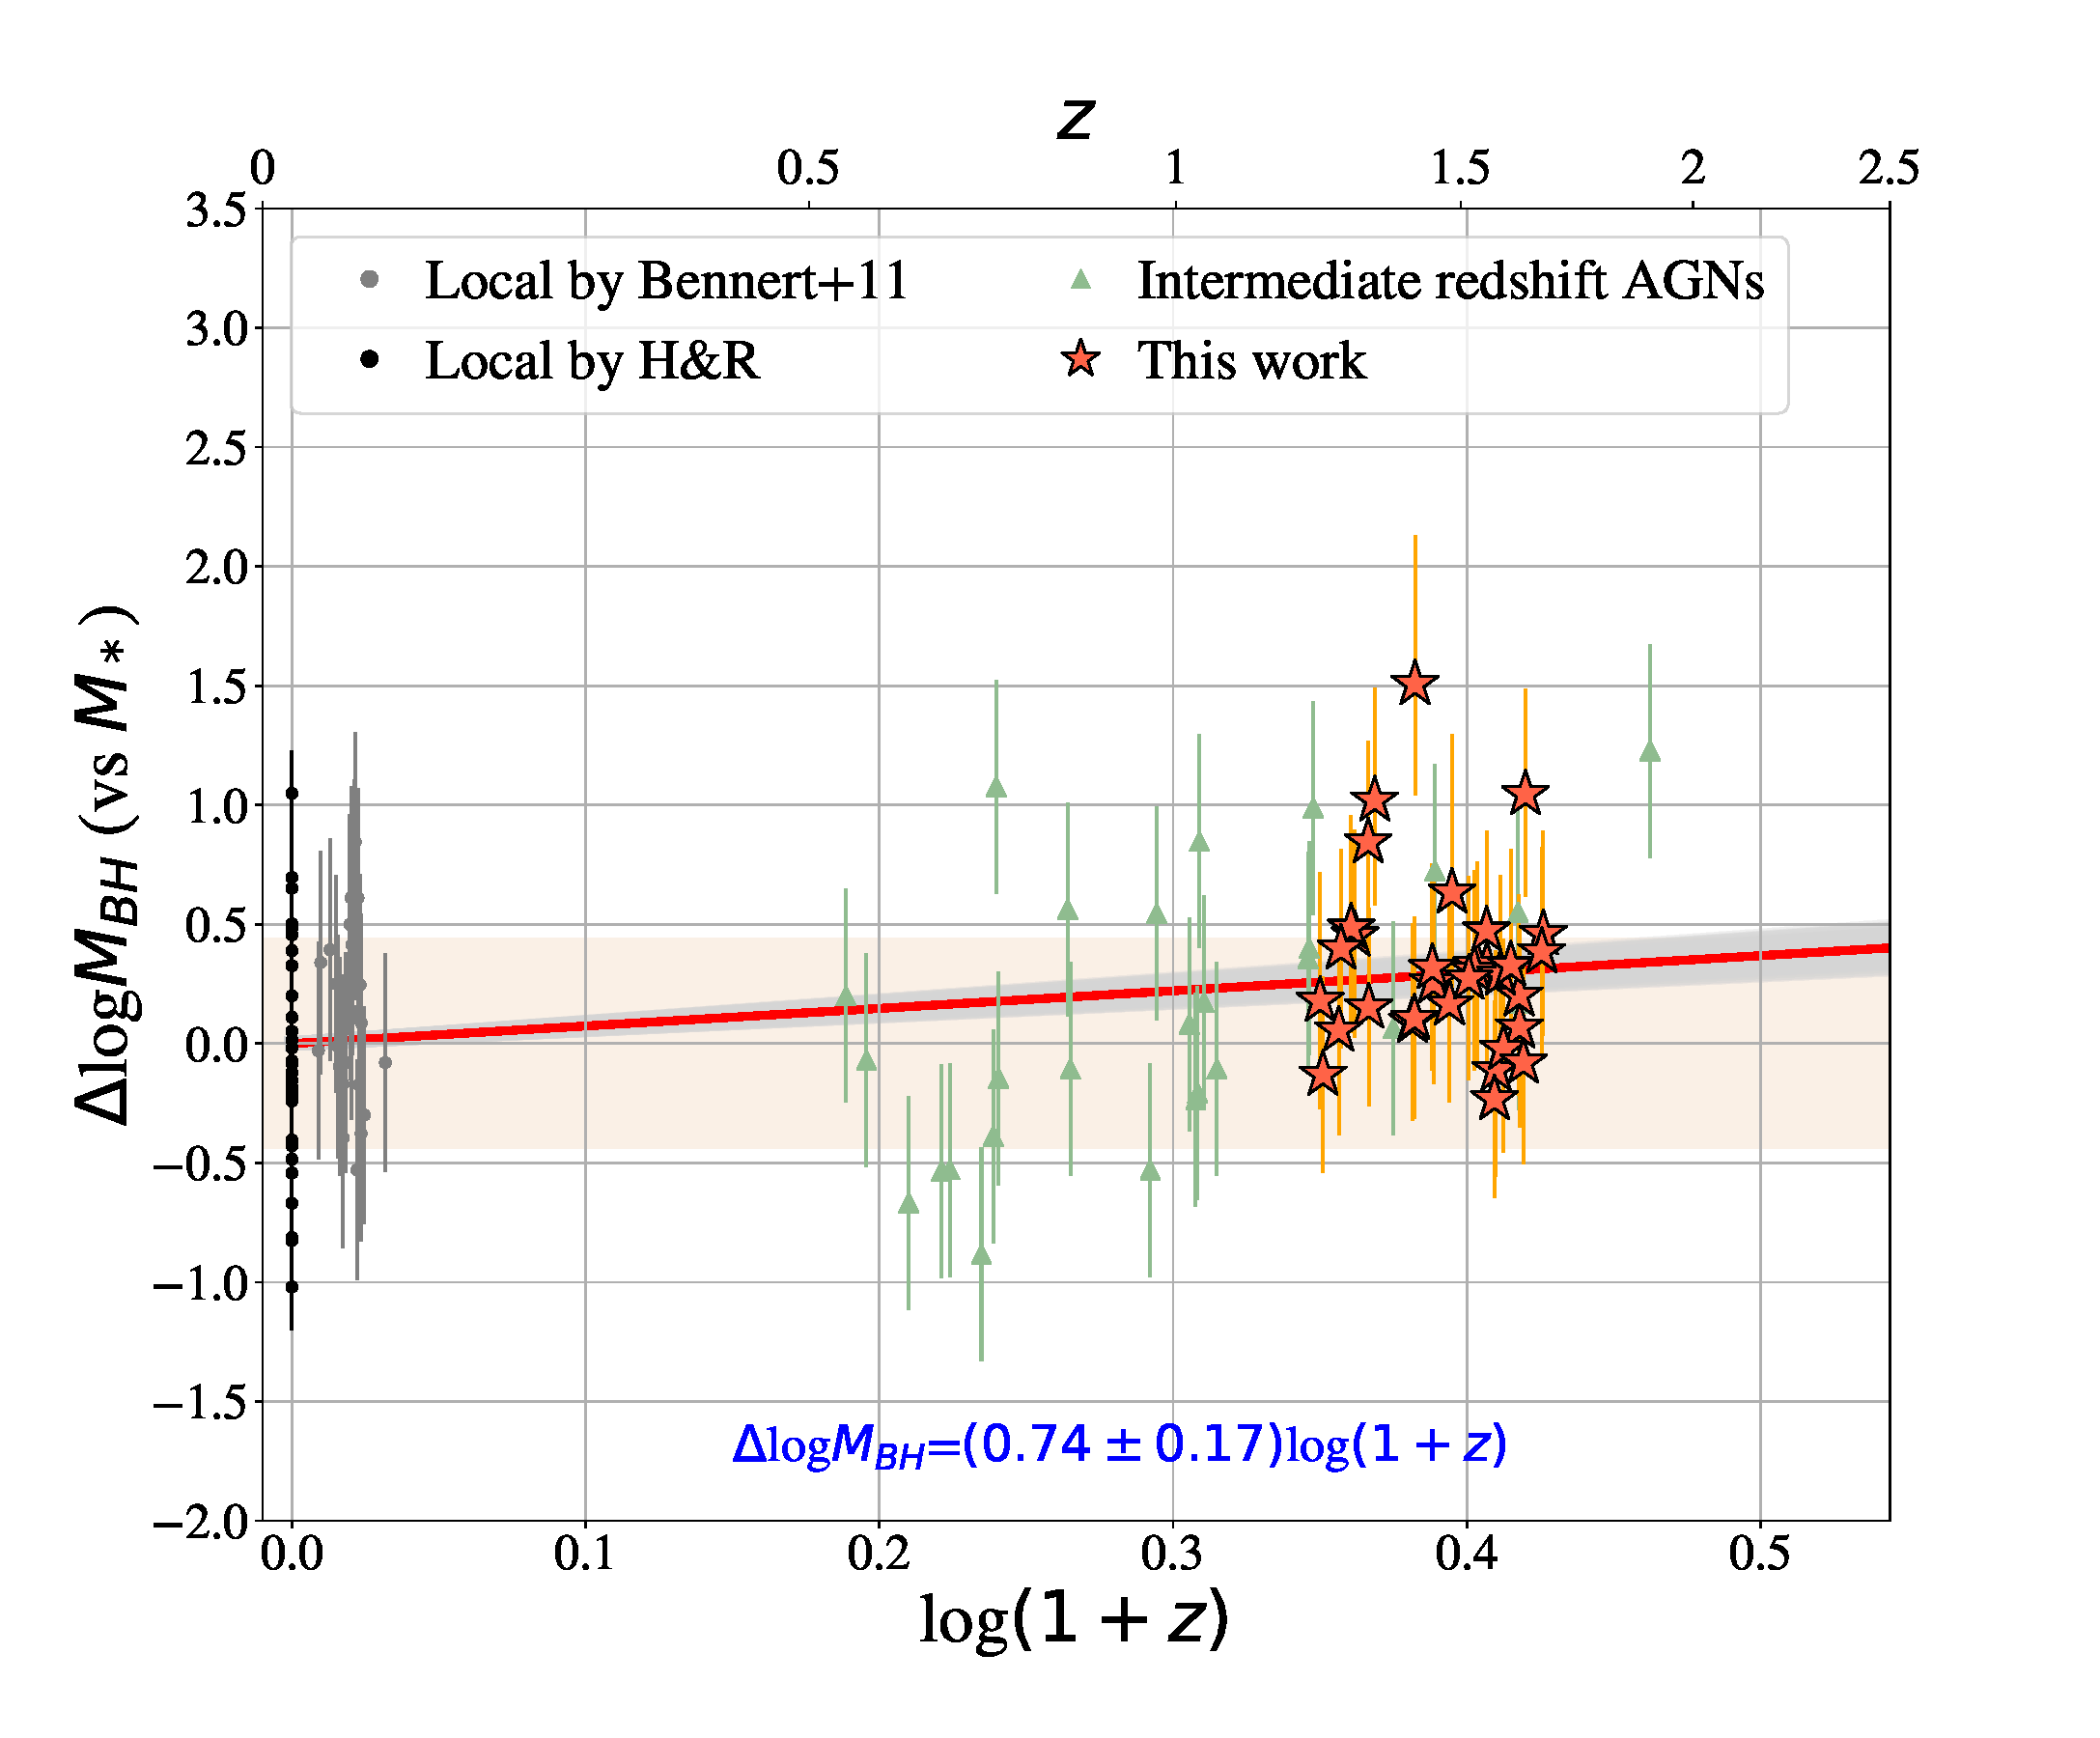
\includegraphics[width=0.5\textwidth]{fig/MBH-Mstar-vz_style1.pdf}}&
{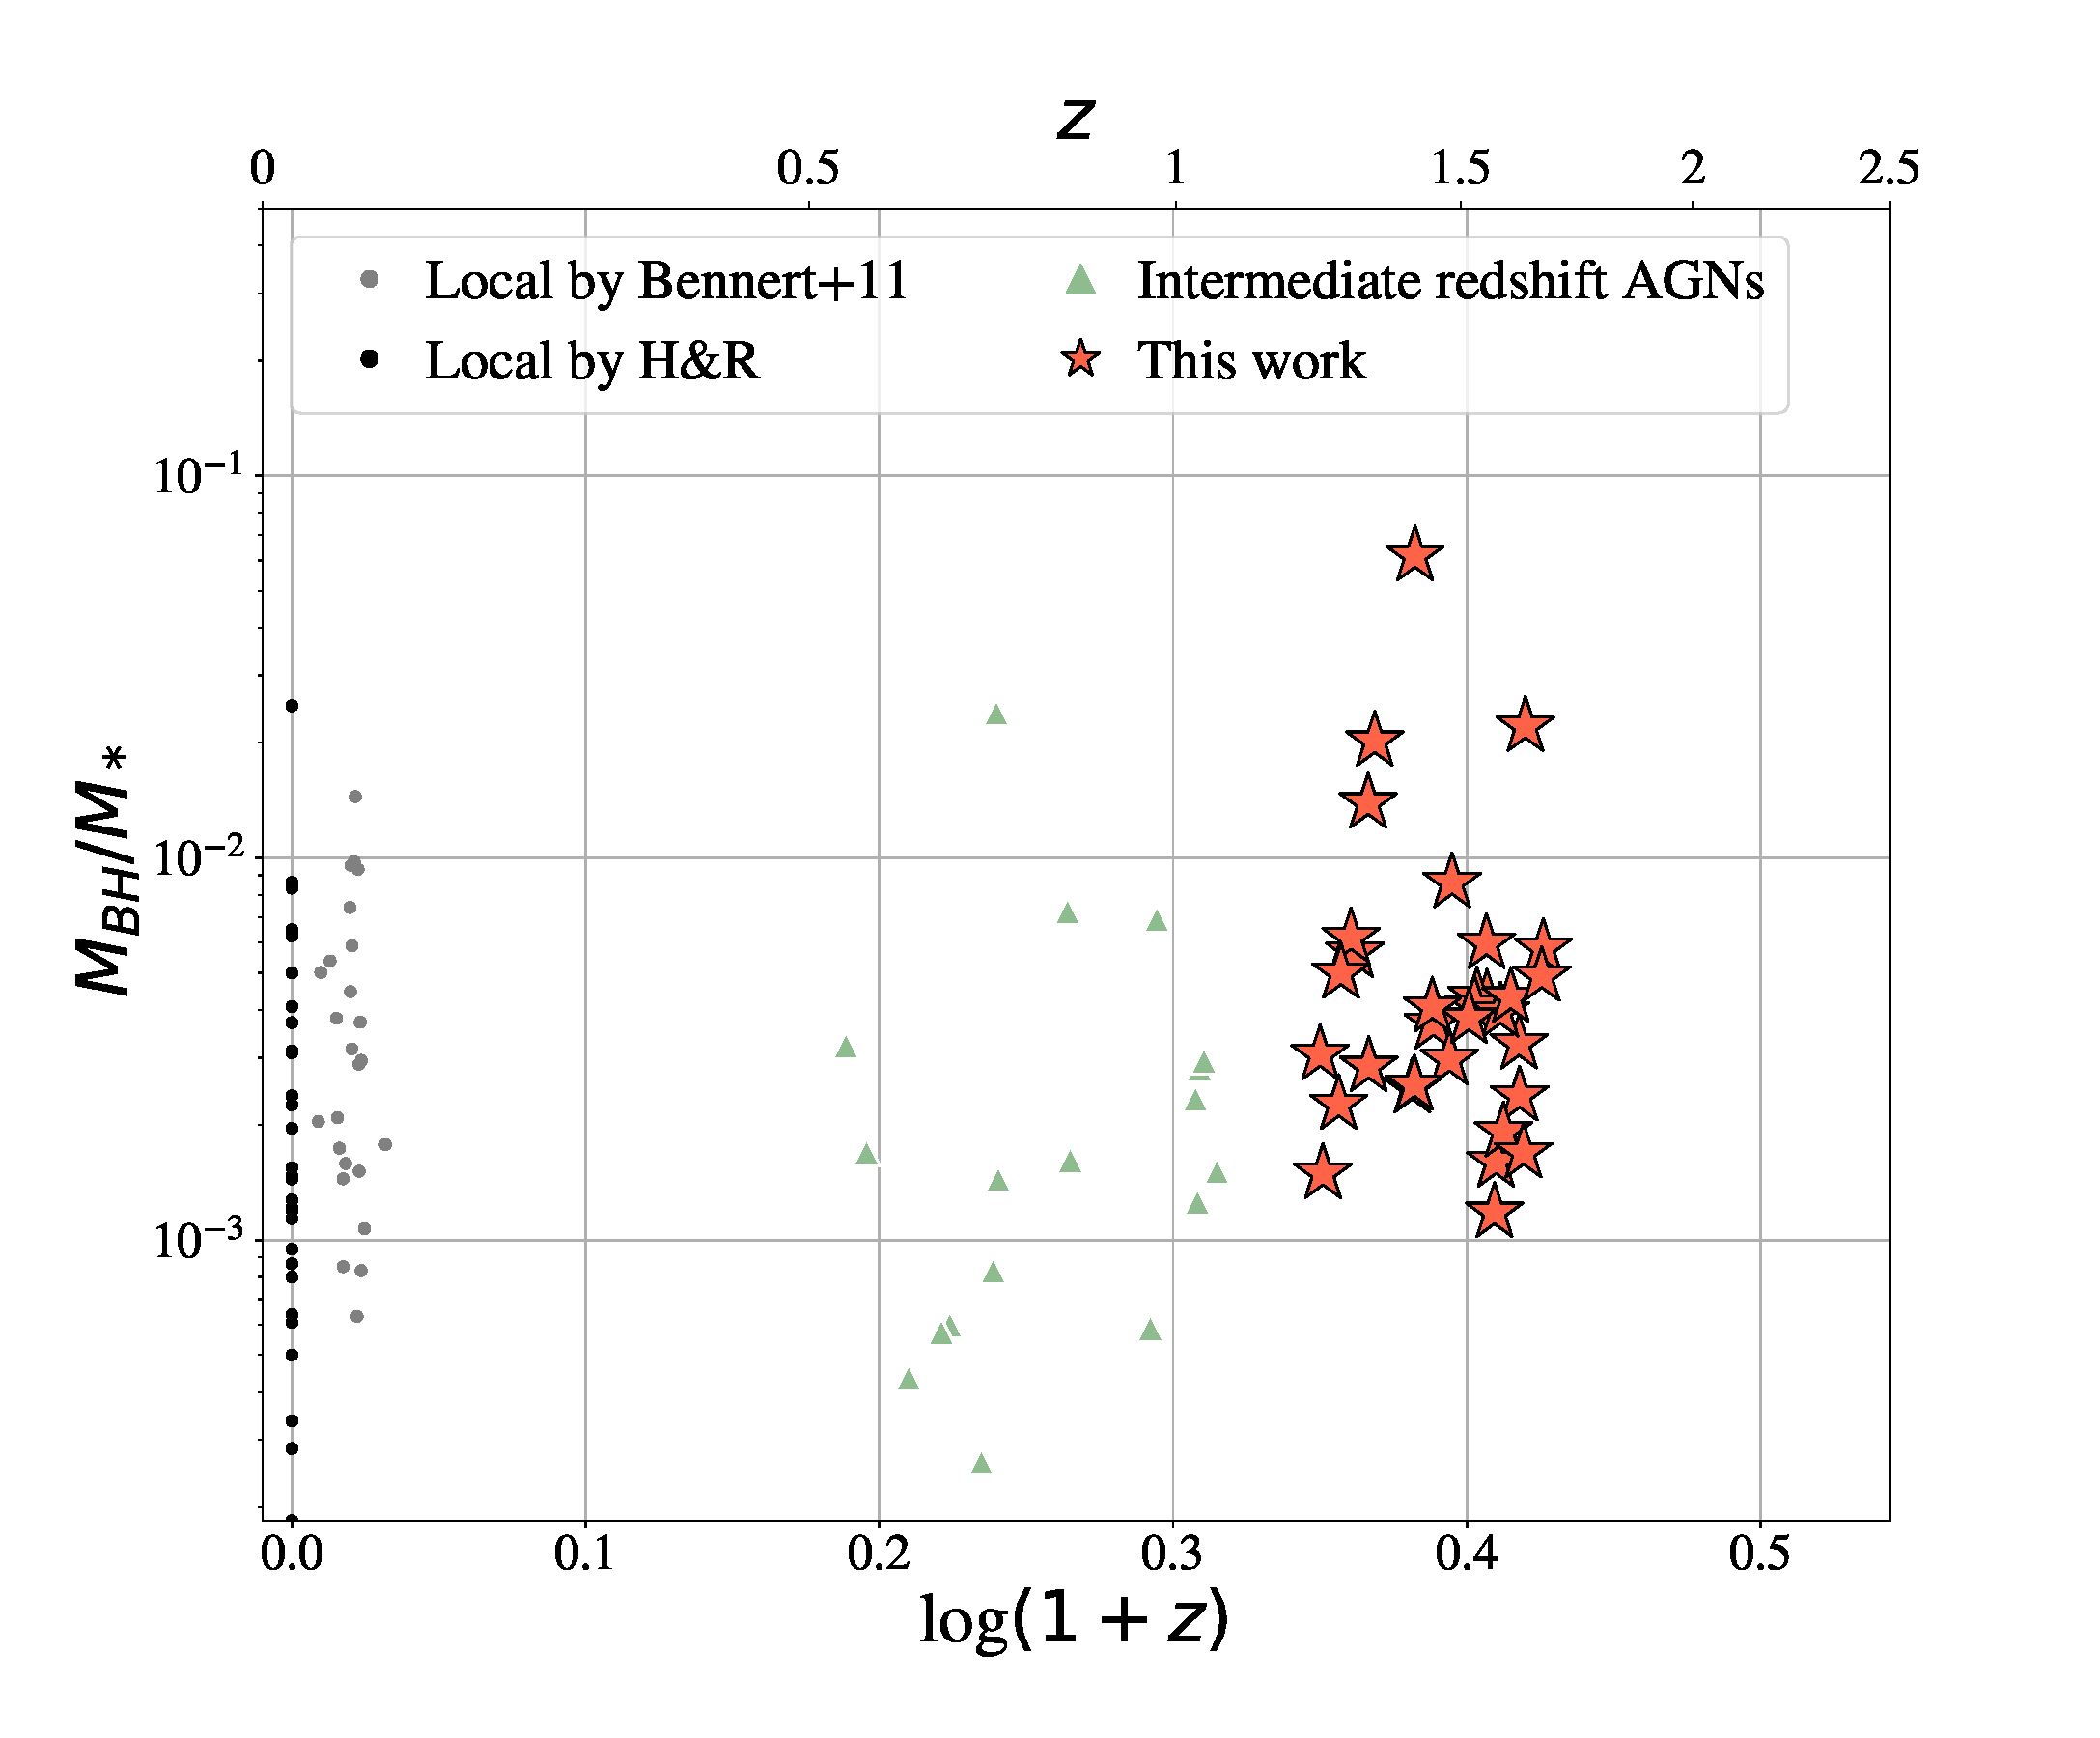
\includegraphics[width=0.5\textwidth]{fig/MBH-Mstar-vz_style0.pdf}}\\
\end{tabular}
\caption{\label{fig:MM-vz} 
Left: Offset in  $\log($\mbh$)$ (vs. \smass) as a function of redshift. The orange band is the intrinsic scatter of local linear relation. The red line and gray band are the best-fit and $1\sigma$ offset fitting by Equation~\ref{eq:offset} using our 32 high-$z$ AGNs.
Right: \mbh/\smass\ as a function of redshift. 
We use green open circles to show the expected shifting of the median value of the $\Delta \log$\mbh\ before and after consider the selection effect using framework by \citet{Schulze2011} in Section~\ref{sec:sf_framework}.}
\end{figure*} 

%{\bf [Include a full paragraph on the scatter]}
As shown in these panels, the scatter of the high-$z$ correlation presents a similarity to the local relation. To quantitively make this comparison, we calculate the scatter of their offset value, based on Equation~\ref{eq:infer_value}, and obtain $0.33$ for high-$z$ and $0.40$ for local samples, respectively. This result is against the scenario where the random merger is the origin of the correlation \citep{Peng2007}, indicating that there is likely to be a connection between the SMBHs and their host galaxies during their formation.

%\begin{figure}
%\centering
%{\includegraphics[width=0.5\textwidth]{fig/MBH-Mstar-vz_subsample.pdf}}
%\caption{\label{fig:MM_restsample} 
%Same as Figure~\ref{fig:MM-vz}, left, but excluding the 3 outliers systems. The result shows the evolution still exist among the other 29 AGN sample.
%}
%\end{figure} 


%We summarize the inference of $\gamma$ using different combination of sample in Table~\ref{table:diff_sample_gam}. All the $\gamma$ by the observed \mbh-\smass\ are inferred as positive, indicating that the growth of the black hole predates that of the host bulge. 


\subsection{Taking into account the selection function}
\label{select_eff}

In Section~\ref{sec:sf_framework}, we used the Bayesian framework introduced by \citet{Schulze2011} to show that in the case of no intrinsic evolution of the correlations we would expect to measure an offset corresponding to a $+0.21$~dex bias in the inferred $\Delta \log$\mbh, owing to our selection function. Interestingly, this bias could account for the majority of the observed offset as obtained in the \mbh-\smass\ correlations in last Section. %~\ref{sec:mm}.
To illustrate the expected bias, we use green open circles to show the corresponding shift of the observed points if one were to correct for this bias in Figure~\ref{fig:MM-vz}. We also show, in Figure~\ref{fig:offset_hist}, the histogram the $\Delta \log$\mbh\ by the high-$z$ sample and compare to the local ones. 
The plots show that the correlations between \mbh\ and host galaxy total stellar mass or luminosity could be consistent with those of the local samples given the uncertainties and selection function



\begin{figure}
\centering
{
\includegraphics[width=0.5\textwidth]{fig/hist_offset.pdf}
}
\caption{\label{fig:offset_hist} 
Histogram of the $\log($\mbh$)$ offset for the local samples and our 32 high-$z$ sample. The gray/red vertical line shows the mean value of the offset for the high-$z$ sample, before/after considering the selection effect. The median value of the offset are very close to the mean value ($+0.3$).
%TT: we need to show the mean, not the median. Or at least both. The median excludes the pull from the higher points, which are probably what drives the inference later on, so for a proper comparison we need to include both. 
}
\end{figure} 

%Our conclusion is that the considering the selection effect using framework by \citet{Schulze2011}, we get consistent \mbh-\smass\ with the local sample.

In order to further evaluate the ``true" underlying evolution and its uncertainty, corrected for selection effects, taking into account the actual observations, we adopt an independent method based on the approach introduced by \citet{Tre++07} and developed by \citet{Park15} and \citet{Ding2017b}. The method parametrizes the evolution of the correlations between \mbh\ and host galaxy properties as an offset from the local one $\gamma$ and an intrinsic scatter \sint, which can be a free parameter or tied to the local relation. It then imposes a selection function in \mbh\ and calculates the intrinsic parameters of the model given the observations. In practice, we start from the local black hole mass function and the evolution model, generate mock samples using a Monte Carlo approach, apply the selection function and compare with the data to generate the likelihood. To illustrate the importance of the intrinsic scatter in the selection effects, we adopt both uniform (flat) prior and lognormal prior for \sint. 
Note that this method assumes a narrow Eddington radio distribution which is different to the one by \citet{Schulze2011}, as described in Section~\ref{sec:sf_framework}. Also, this method adopts the local black hole mass function rather than high-$z$ BH mass function. These differences have a second order effect and could be responsible to the different magnitude of the selection effect. On the other hand, this method probes the importance of the scatter at high-$z$, which is complementary. %Thus each is complementary that should be stressed maybe in the abstract (see my suggested change).



Combining the 32 AGNs together with the intermediate redshift sample, we present the inferred  $\gamma$ and \sint\ in the two-dimensional planes in Figure~\ref{fig:select_effect}. The plots show that the inferred evolution is uncertain and depends crucially on the intrinsic scatter, especially when applying a luminosity evolution for the host (see Appendix~\ref{sec:ml-ev}). Assuming the lognormal prior \sint, to mimic the assumption of the method discussed in Section~\ref{sec:sf_framework}, one sees that the best estimate of $\gamma$ is positive, but the 95\% confidence intervals extend to zero. Thus one cannot conclude that evolution is significantly detected in our data. 
When relaxing the prior on \sint\ we find that the scatter is consistent with being as low as in the local samples, with a one-sided interval including zero and peaking at around 0.5~dex. 
We also study the selection effect by only consider the new 32 AGNs, result in a higher evolution trend with a higher value of $\gamma$. We show all the result of the $\gamma$ and \sint\ in Table~\ref{table:gamma_sf}.

A simple check using our a-priori estimate of the bias, yields a similar result. The mean offset of the sample of 32 objects from the local relationship is $0.34\pm0.06$ dex, which would correspond to $\gamma=0.85\pm0.15$. However, after correcting for the selection bias ($0.21$~dex, see Section~\ref{sec:sf_framework}), the offset reduces to $0.13\pm0.06$ and thus $\gamma=0.33\pm0.15$, mildly positive but not significantly so, and consistent with the a posteriori method within the error bars and the uncertainty in the correction. We also note that the distribution of offsets shown in Figure~\ref{fig:offset_hist} displays a positive asymmetric tail. Whereas we expect the negative tail to be suppressed by our selection function, and thus it should be accounted for in our treatment, it is true that those three objects contribute a large fraction of the object. If one computes the median offset instead of the mean, the offset is almost completely consistent with the expected bias. Larger samples are needed to establish whether the positive tail is real or due to small sample statistics. 

\begin{figure*}
\centering
\begin{tabular}{c c}
\subfloat[\mbh-\smass, flat prior]
{\includegraphics[width=0.5\textwidth]{fig/MM_MC_seleff_flatprior.pdf}}&
\subfloat[\mbh-\smass, lognormal prior]
{\includegraphics[width=0.5\textwidth]{fig/MM_MC_seleff_lognormprior.pdf}}\\
\end{tabular}
\caption{\label{fig:select_effect} 
Taking selection effects into account, figure illustrate the constraining on the evolution factor $\gamma$ of \mbh-\smass\ relation by Equation~\ref{eq:offset}, with intrinsic scatter \sint, using Monte Carlo simulation. The adopted sample includes our 32 AGNs and the intermediate redshift AGNs, using flat prior of \sint\ (left panel) and lognormal prior (right panel).
}
\end{figure*} 

\subsection{\mbh-\bmass\ relation}\label{sec:bh_bulge}

The local sample of inactive galaxies used in this analysis is mainly comprised of bulge-dominated galaxies and the adopted \smass\ are equivalent to their bulge masses. That is, in previous sections, we are comparing the \mbh-\smass$_{\rm ,total}$ relations in the distant universe to the \mbh-\smass$_{\rm ,bulge}$ relations locally. Considering that a significant stellar component of the high-$z$ AGNs have a disk component (i.e., AGN hosts with fitted \sersic\ index close to 1),  \smass$_{\rm , bulge}$ will be smaller than \smass$_{\rm ,total}$.

Given that the structure of our 32 AGN hosts are similar to inactive
galaxies at the same redshifts and stellar masses
(Section~\ref{sec:result-hosts}), we expect their B/T ratios follow
a similar distribution which can estimated using the single-\sersic\
index \citep{Bruce2014}. With this estimation, we can infer the
bulge stellar mass of our AGN host.

Under these assumptions, we first establish the relation between the
single-\sersic\ index and B/T ratios for CANDELS inactive galaxies
at the similar mass level, i.e \smass$\in [9.0, 11.5]$, using B/T
measured by \citet{Dimauro2018}. Then, we calculate the average B/T
ratio at different \sersic\ index to construct a relation for our
use, as shown in Figure~\ref{fig:BT-n_relation}. Taking this
relation, we estimate the B/T of our AGN sample using the \sersic\
index as proxy and infer their \smass$_{\rm, bulge}$ from the total
stellar mass. 

We can now compare this \smass$_{\rm, bulge}$ to that
of the black hole \mbh. As expected, we find a stronger offset of
$0.65\pm0.11$~dex in \mbh/\smass$_{\rm, bulge}$ with respect to the
local relation, which corresponds to an evolutionary trend with
$\gamma = 1.63\pm0.27$. Since selection effects are independent of B/T in
our framework we can apply our a-priori estimate of the selection
effect correction by removing 0.21~dex, leaving a significant offset
of $0.44\pm0.11$.

Even with the uncertainty associated with our estimate of the
bulge-to-total ratio it is clear that there is significant evolution
in the \mbh\ -- \smass$_{\rm , bulge}$ relation, considering the
marginal evidence for evolution in the \mbh-\smass$_{\rm, total}$
relation and that our galaxies are not pure bulges. This finding
confirms with higher fidelity the conclusion by \citet{Bennert11}
based on optical data of a smaller sample of 11 objects in the same
redshift range \citep[see][for similar results.]{SS13, Jah++09, Cisternas2011} 

\begin{figure}
\centering
{
\includegraphics[width=0.5\textwidth]{fig/BT_relation.pdf}
}
\caption{\label{fig:BT-n_relation} 
Relation between bulge-to-total stellar mass ratio and single-\sersic\ index using CANDELS inactive galaxies with \smass$\in [9.0, 11.5]$. The red curve is the inferred specific relation taking the average B/T ratio at different \sersic\ index, used as proxy to infer the B/T for our AGN sample.
}
\end{figure} 

\begin{figure*}
\centering
\begin{tabular}{c c}
{\includegraphics[width=0.5\textwidth]{fig/MBH-Mbulge-style1.pdf}}&
{\includegraphics[width=0.5\textwidth]{fig/MBH-Mbulge-style0.pdf}}\\
\end{tabular}
\caption{\label{fig:MM_bulge-vz}
Same as Figure~\ref{fig:MM-vz}, but for \mbh-\bmass\ relations.}
\end{figure*} 


\section{Final technical remarks}
\label{sec:dis}


%{\color{blue}
%\subsection{The origin of the offset}
%{\color{red}[Xuheng:  Given their larger uncertainty, do we still want to present these figures?]}
%We seek for the cause that could raise the evolution in the BH and host galaxy correlations at high redshift. We consider if the offset is related to the AGN activities. The straightforward way is to study such offset, i.e. $\Delta \log \mathcal M_{\rm BH}$, as a function of \mbh\ and Eddington ratios, showing in Figure~\ref{fig:offset_vs_MBH_edd}. Interestingly, we visually see the trend that the offset turns to be larger with at value of \mbh. However, at higher Eddington ratio, the offset turns to be lower.
% {\color{red} Some interpretations need to be presented.}
%}
%\begin{figure*}
%\centering
%\begin{tabular}{c c}
%\subfloat[Offset of the \mbh-\smass\ relation as a function of \mbh.]
%{\includegraphics[height=0.5\textwidth]{fig/offset_vs_MBH.pdf}}&
%\subfloat[Offset of the \mbh-\smass\ relation as a function of Eddington ratio.]
%{\includegraphics[height=0.5\textwidth]{fig/offset_vs_Edd.pdf}}\\
%\end{tabular}
%\caption{\label{fig:offset_vs_MBH_edd} 
%Illustration of the offset for high-$z$ \mbh-\smass\ sample as a function of \mbh\ (left) and Eddington ratio (right).}
%\end{figure*} 
%

\subsection{Systematic errors}

In this work, we use the start-of-the-art techniques to measure the host galaxy flux separating it from that of the point source. The fidelity of the host galaxy magnitude is high as demonstrated by the robustness with respect to the choice of PSF which is the main source of uncertainty. However, we introduce some uncertainty by adopting a simple stellar population template to derive the rest-frame R-band luminosity and stellar mass for the full population. In principle, if we had more information, we could improve on this source of uncertainty by a adopting a specific stellar population model for each. However, considering that the host magnitude in the \hst/ACS band is faint (host-to-total flux ratio $< 30\%$), the individual color that we measure is insufficient to further discriminate between templates and thus we adopt a single one for simplicity and to facilitate reproduction of our work.

%We highlight that, in this particular paper, we focus most on the decomposing of the AGN image to present our inference of the host. With the host inference, we then carry out a rapid analysis of the \mbh\ and host properties relations. The measurements incorporating the ground-based photometry and the comparison with the simulations are presented in our companion paper.

In any case, We stress that the uncertainty in the scaling relations is dominated by the single epoch black hole mass estimates, and not by uncertainties in the photometry or stellar mass estimates. Thus, the choice of template is a vastly subdominant source of error. A posteriori, the fact that the intrinsic scatter we observe is not larger than the one in the local universe is consistent with this statement.

\subsection{Systematic errors related to the choice of local anchor}
\label{sec:local_sys}

To compare our high-$z$ sample to the local relation, we adopt the local measurements by \citet{Ben++10, Bennert++2011} and  \citet{H+R04}. In the literature, other analyses of the local sample are available which could also be considered as the local anchor. We note that the different local samples have inconsistencies which could affect our measurement of the co-evolution. Since the local correlations are used to calibrate the single epoch black hole mass estimates, one needs to be self-consistent in the choice of local anchors and calibration of black hole mass estimators. Unfortunately, this is a thorny issue, since not all the local correlations are mutually consistent especially when considering different galaxy properties like luminosity stellar mass and velocity dispersion.

To illustrate the problem, we compare our local \mbh-\smass\ sample to that published in \citet{Kormendy13} (hereafter K13). We find that the \mbh-\smass\ measurements in K13 have a global $\sim+0.3$~dex offset relative to our local sample. Note that a $+0.3$~dex difference could totally erase the $\Delta\log$\mbh\ for the high redshift sample as described in last section, if it were independent from the black hole mass calibration.

However, the \mbh-\sigstar\ relations by K13 are also offset by  $\sim+0.3$~dex with respect to those given by \citet{Woo2010}, which is the baseline for our adopted black hole mass estimators. Thus, if we were to adopt the K13 normalization instead, the \mbh\ of all the AGN sample should be increased by $\sim$0.3~dex. As a result, adopting a different local anchor would only globally affect the level of the \mbh\ to local and high-$z$ sample at the same time, with the result of leaving $\Delta\log$\mbh\ unchanged.  

In conclusion, whereas the uncertainty in the local anchor does not affect our measurement of evolution, it is important to keep in mind this issue in evolutionary studies and verify that the measurements are as self-consistent as possible in the local and distant universe. In order to further reduce the uncertainty, one should perform a self-consistent measurement with identical techniques and data quality both in the local and distant universe. This effort is currently in progress and when completed should enable us to completely eliminate this source of uncertainty \citep{Bennert11,Harris2012, Bennert2015}.

%\begin{figure}
%\centering
%{\includegraphics[width=0.5\textwidth]{fig/local_MM_comparison.pdf}}
%\caption{\label{fig:local_MM_comp} 
%The local \mbh-\smass\ relations from different literature. The black and red line are the best-fit linear relation using the sample by combining B11+HR04 and B11+ K13, respectively, showing a 0.3~dex offset in the intercept value.
%}
%\end{figure} 

\section{Conclusions} \label{sec:sum}

We studied the evolution of the correlations between the supermassive black hole and their host galaxies using new measurements of 32 X-ray selected AGNs at $1.2<z<1.7$. Near-infrared spectroscopic observations with Subaru/FMOS of the \halpha\ emission line are available that provide reliable BH masses. To obtain the properties of the AGN host galaxies, we performed an image decomposition using the state-of-the-art techniques on \hst/WFC3 IR data to obtain high-resolution imaging of the AGN and its host. This required us to collect PSF-stars across all the fields to build to a library of PSFs. Using the state-of-the art image modeling tool \lenstronomy, we decomposed the AGN image in 2-D plane taking each PSF in the library. We obtained the host properties (i.e., host flux, effective radius, \sersic\ index) using a weighted arithmetic mean based on the inference from the eight top-ranked PSFs. With additional \hst/ACS image in the optical, we identified the appropriate stellar population and derived the rest-frame R-band luminosity (\lhost) and stellar mass (\smass) of the host with the corresponding mass-to-light ratio.
We then determine the mass relations at high-$z$ and establish any signs of evolution by combining our high-$z$ measurements with local and intermediate redshift samples from the literature~\citep{Park15, Bennert11, SS13, Cisternas2011}. 

We find the average ratio between the mass of a supermassive black hole and either their total host luminosity or total stellar mass is larger at $z\sim1.5$, by factor of $\sim2.2$ and $\sim2.5$ respectively, as compared to that in the local universe. However, taking into account selection bias, these correlations are
consistent with the local universe within the 95\% confidence limits. 
%Therefore, for a fixed black hole mass, the host galaxy total stellar mass and luminosity could be larger than in the local universe by a factor of two, or equal to the local universe which is consistent with no evolution.
Even with the remaining uncertainties in the corrections for selection, we are confident that any evolution in the \mbh/\smass\ relation is at the most a factor of two with the case of no evolution entirely plausible.

Considering the bulge component instead to be the main driver of the local correlations \citep{Bennert11, Woo++08}, we find that our high-$z$ AGN sample has significantly lower mass/luminosity bulges at fixed black hole mass than in the local universe. Comparing to their \mbh, we find evolution with the ratio evolving as $(1+z)^{1.63\pm0.27}$, which is significant even accounting for selection effects. We caution that the evolution of the bulge component is more uncertain than our measurement of the total galaxy components, since it is based on an estimate of the B/T ratio from the measured Sersic indices from a matched sample of inactive galaxies. Nevertheless, since the signal is stronger than for the integrated quantities, the measurement is more significant even in presence of larger uncertainties.
Thus, we can conclude that the BHs 8-10~Gyrs ago reside in bulges which are less massive/luminous than today \citep[see also][]{Bennert11,Park15}, even though a proper measure of the bulge mass at high-$z$ may need to wait for the next generation ground-based 20-30m class telescopes. 

Given that the total-\mbh\ relation is closer to or consistent with the local relation, the inferred evolution of the bulge-\mbh\ correlations is qualitatively consistent with a scenario where the assembly of the black hole predates that of the bulge, which is completed by the transfer of stellar mass from the disk via mergers or secular processes \citep{Croton2006}. The stellar mass need to build the bulge appears to be present in the disk component at high-$z$.

Of further interest, the scatter in the \mbh-\smass\ ratios at high-$z$ is similar to the local one. This was unexpected since the measurements of the masses of both the black holes and their hosts should have more uncertainty that local estimates. If true, this may indicate that cosmic averaging of initially unrelated states \citep{Peng2007} are not driving the relation between SMBHs and their host galaxies thus there is likely a connection between the two yet to be fully understood, contenders include AGN feedback or links to common gas reservoirs.

Finally, the forthcoming launch of the {\it James Webb Space Telescope} ({\it JWST}) may provide high-quality imaging data of AGNs at higher redshift (up to $z\sim$7) and thus trace the evolution of correlations at more distant universe. Although, galaxies, as we know, are smaller at high-$z$ thus may remain challenging to detect under the glare of a luminous AGN. In the lower redshift Universe, wide area surveys with Subaru/HSC, LSST and WFIRST offer much promise to build samples for studying these mass ratios and dependencies on other factors (e.g., environment).  

%Our inference indicates the evidence of disk+bulge component, i.e. the ones with \sersic\ $n<2$, and the local comparing samples are bulge dominated sample, we hence conclude that the BHs 8-10~Gyrs ago reside in bulges, if not entire galaxies, which are less massive/luminous than today.

%Towards a better estimation of the evolution of the scaling relations, we address the limitations of this work. First, most of the host-total ration in the \hst/ACS band are low ($<20\%$), the fidelity of the host flux are thus limited at UV band. In addition, when deriving the \lhost\ and \smass, we adopt a universal stellar template to the overall galaxies based on the general inference between UV band and IR band, rather than carry out the SED fitting for each galaxy. Second, the local scaling relations that we currently adopted are not yet solid. We found a 0.3 dex systematic among different local sample \citep{Ben++10, Bennert++2011, H+R04, Kormendy13, Bentz2018}. Tough this systematic might not raise a severe issue in our study of $\Delta\log$\mbh\ (i.e. Section~\ref{sec:local_sys}), a solid sample served as the local anchor is still needed (Bennert et al., in prep). On the other hand, comparing the observational measurements to the ones by the simulation could avoid not only the dependency to the local anchor, but also the bias by selection effect \citep{DeG++15, Khandai2015, Menci2014}. To overcome these limitation, we are incorporating our measurement with the ground-based photometry to derive SED fitting, in order to compare with the sample by simulations, which will be presented in the coming up paper.

%

\clearpage
\section*{Acknowledgments}
Based in part on observations made with the NASA/ESA Hubble Space Telescope, obtained at the Space Telescope Science Institute, which is operated by the Association of Universities for Research in Astronomy, Inc., under NASA contract NAS 5-26555. These observations are associated with programs
\#15115. Support for this work was provided by NASA through grant number HST-GO-15115 from the Space Telescope Science Institute, which is operated by AURA, Inc., under NASA contract NAS 5-26555.

%The authors fully appreciate the discussions with Hyewon Suh, Vardha N. Bennert, Anton M. Koekemoer, Takahiro Morishita and Peter Williams.

XD, SB and TT acknowledge support by the Packard Foundation through a Packard Research fellowship to TT.

{\color{red} More acknowledges to be updated.}

This work has made use of \lenstronomy~\citep{lenstronomy}, {\sc Astropy}~\citep{Astropy}, {\sc photutils}~\citep{photutils}, {\sc TOPCAT}~\citep{TOPCAT}, {\sc Matplotlib}~\citep{Matplotlib} %, {\sc adjustText}~\citep{adjustText}
and standard Python libraries.

\bibliographystyle{apj.bst}
\bibliography{references}

\newpage

\appendix

\section{A. AGN - host galaxy decomposition for the remaining 31 AGNs}\label{sec:restsample}
The AGNs decomposition for the other 31 objects of our sample, presented in the same way as Figure~\ref{fig:AGN_decomp}.

\begin{figure}[ht]
\centering
%\hspace{-5.5em}
{
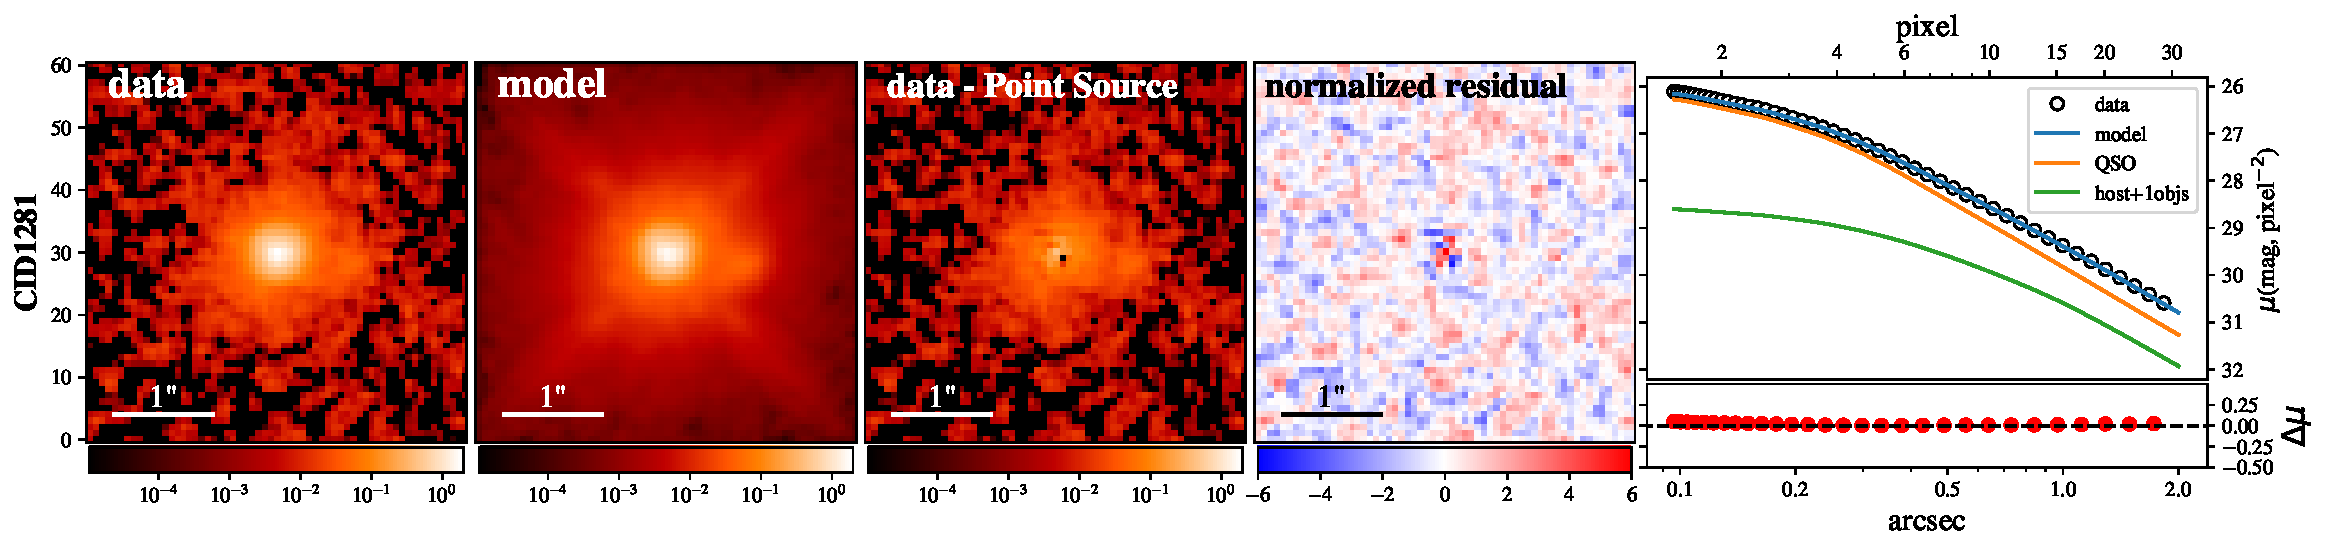
\includegraphics[height=0.25\textwidth]{fig/best_fit_CID1281_SB_profile.pdf}
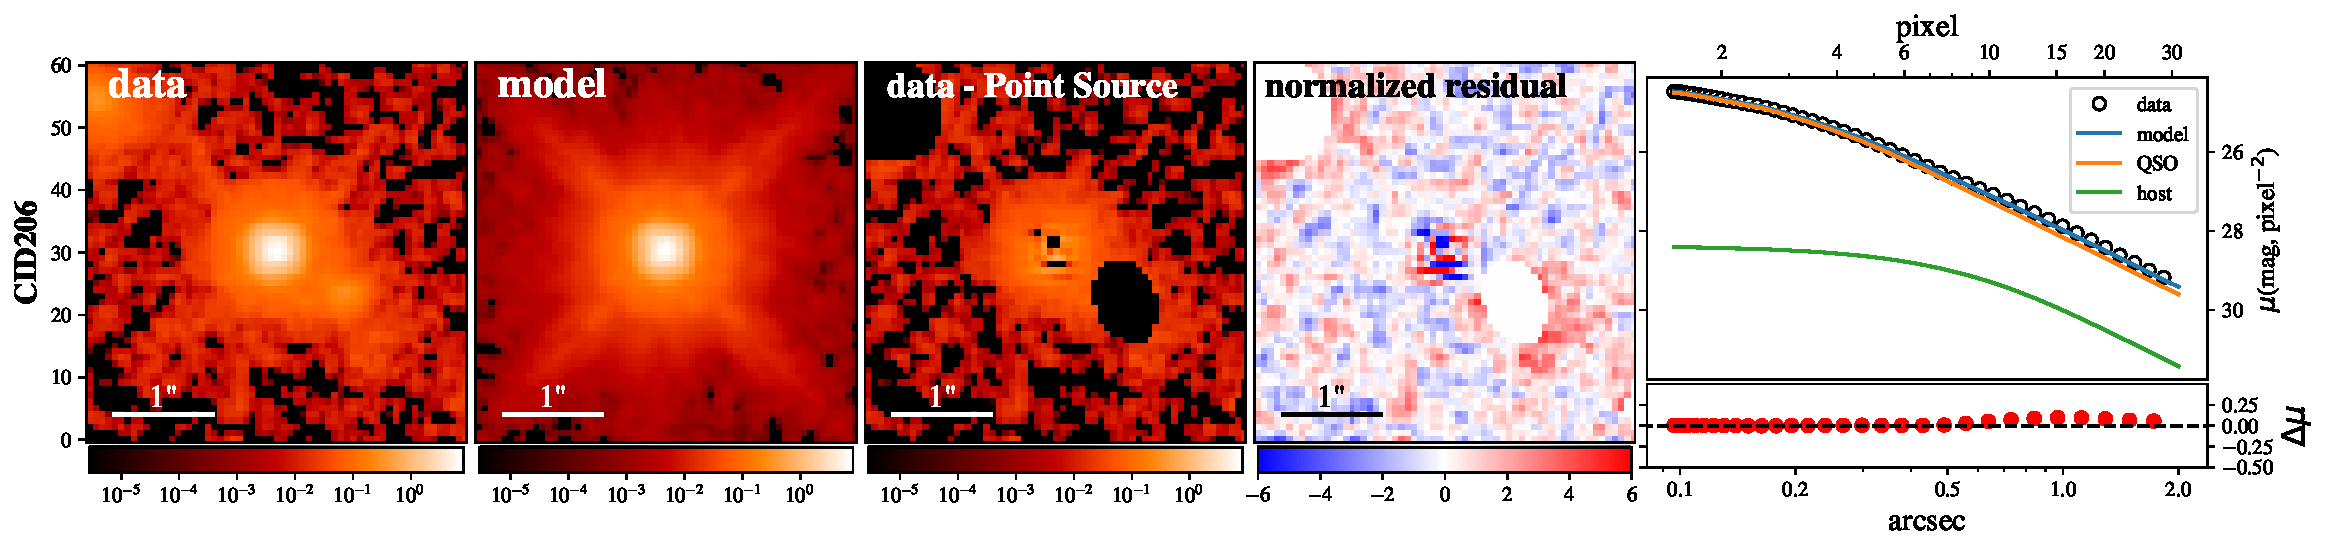
\includegraphics[height=0.25\textwidth]{fig/best_fit_CID206_SB_profile.pdf}
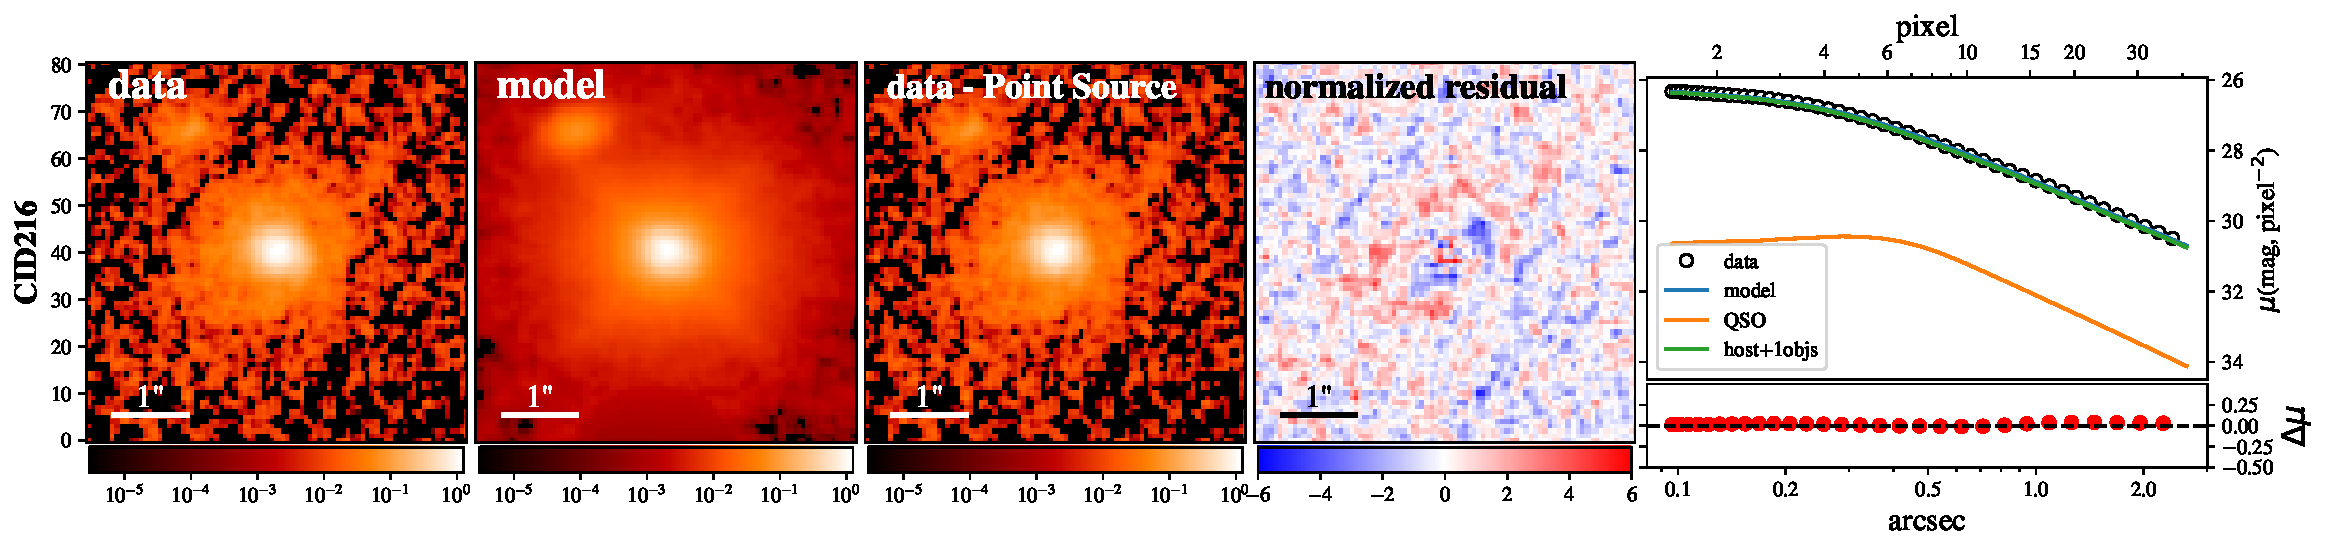
\includegraphics[height=0.25\textwidth]{fig/best_fit_CID216_SB_profile.pdf}
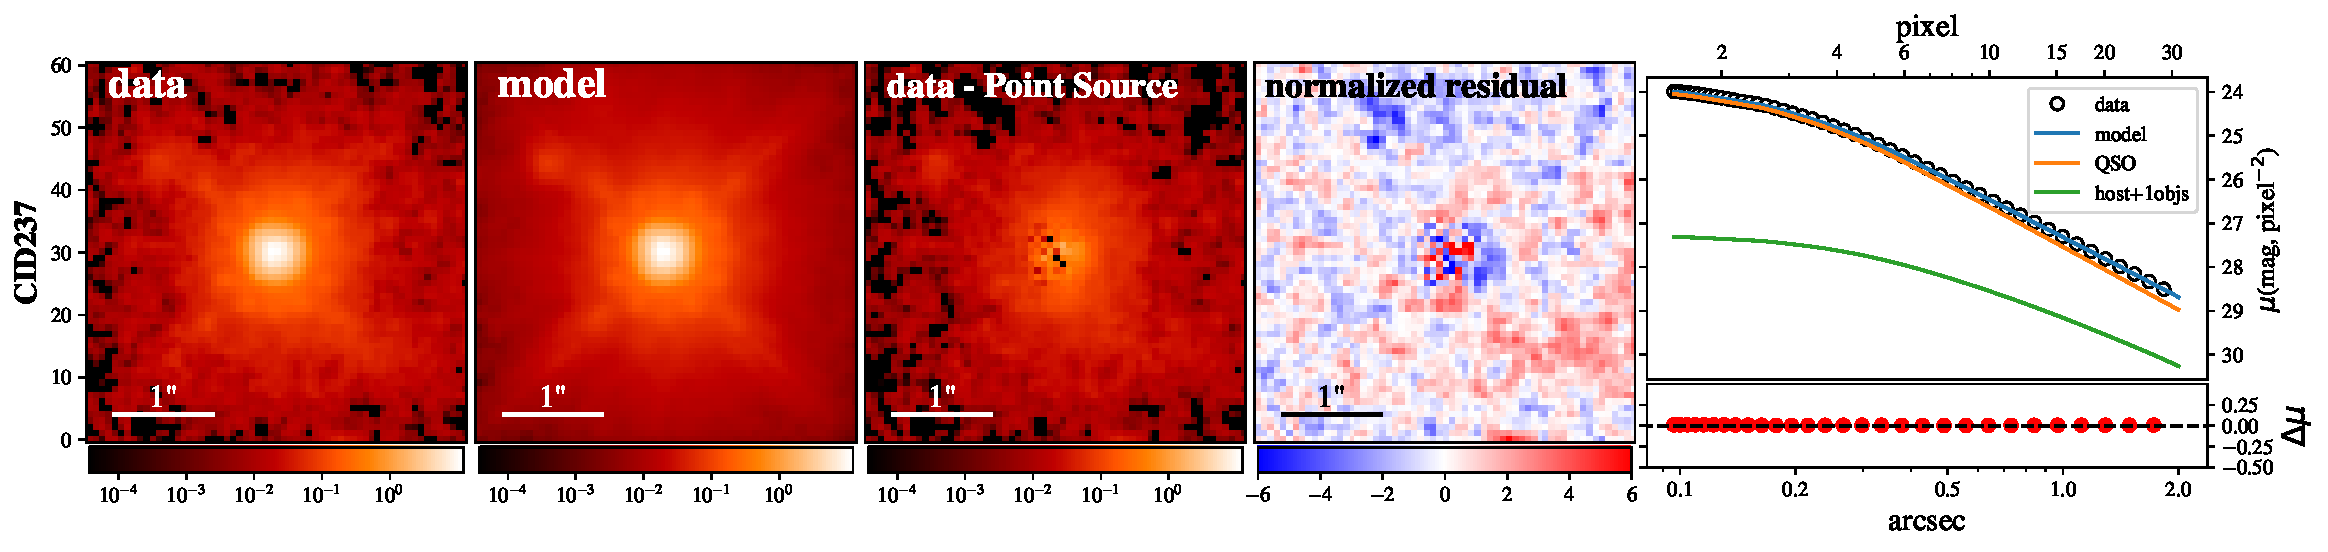
\includegraphics[height=0.25\textwidth]{fig/best_fit_CID237_SB_profile.pdf}
}
\end{figure} 

\begin{figure}
\centering
%\hspace{-5.5em}
{
\includegraphics[height=0.25\textwidth]{fig/best_fit_CID255_SB_profile.pdf}
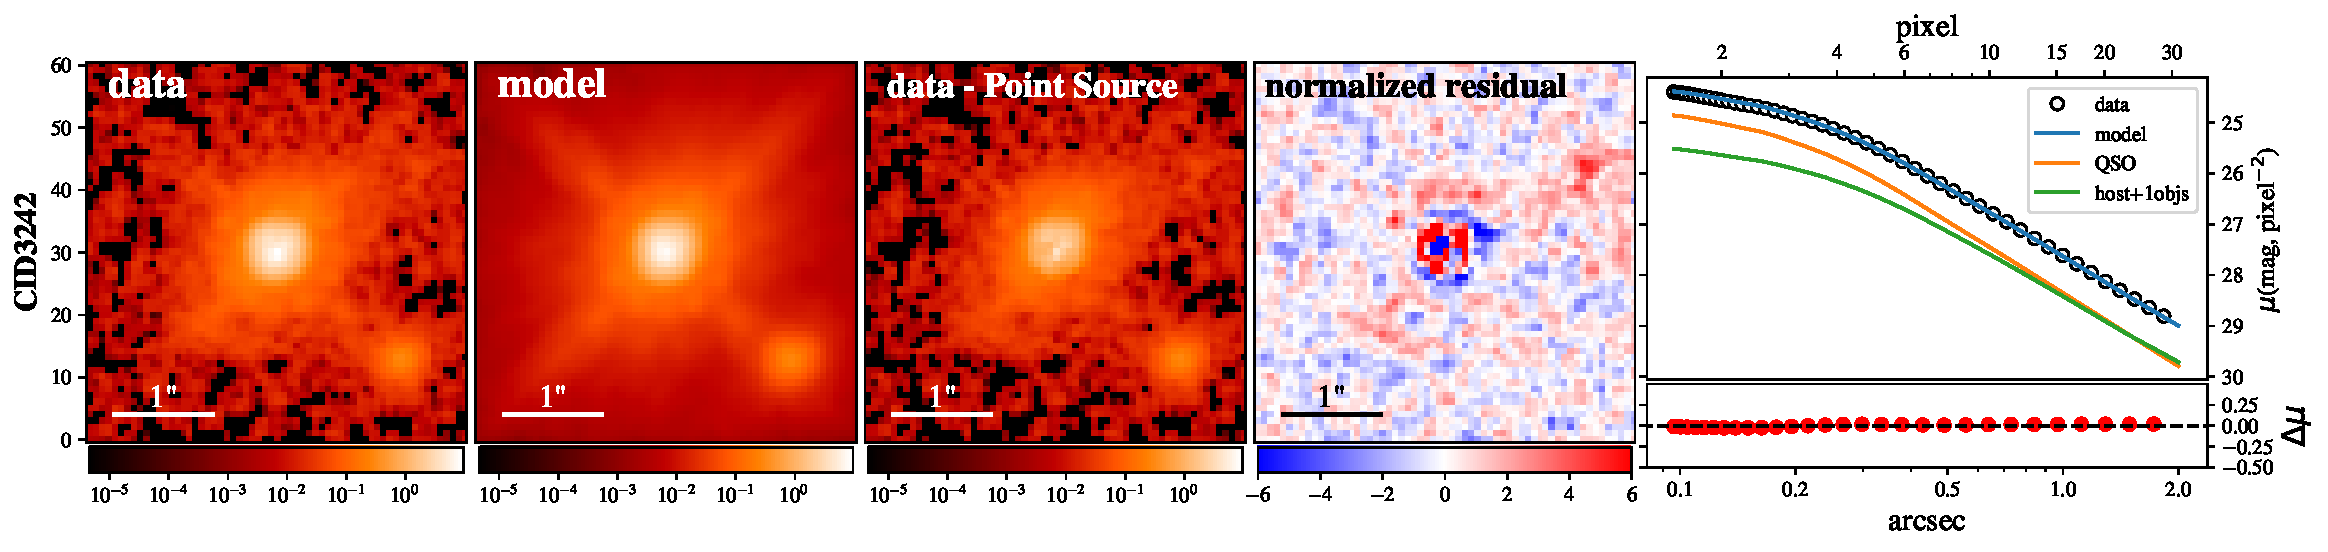
\includegraphics[height=0.25\textwidth]{fig/best_fit_CID3242_SB_profile.pdf}
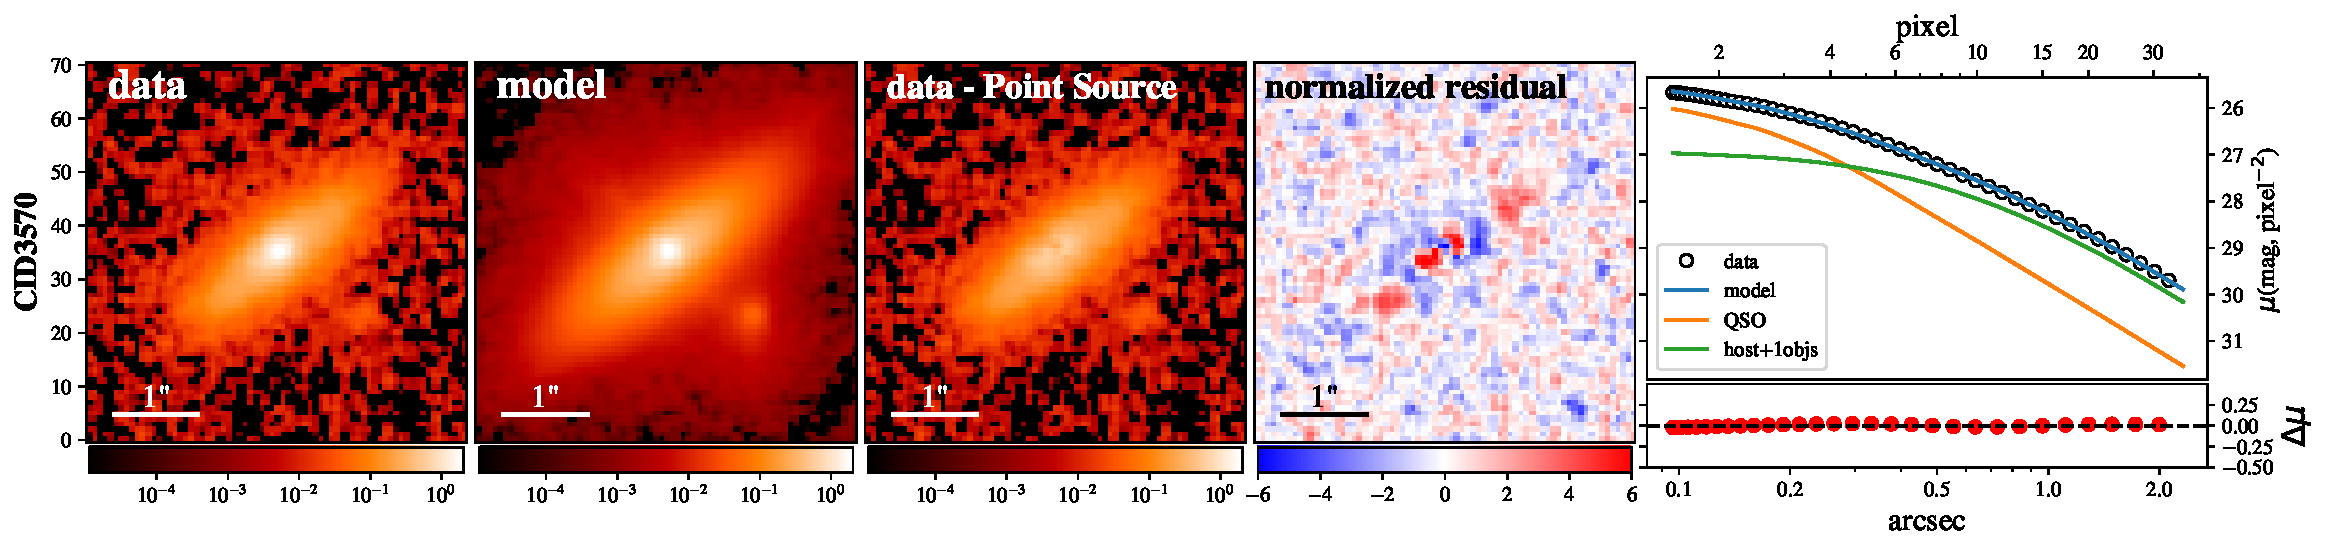
\includegraphics[height=0.25\textwidth]{fig/best_fit_CID3570_SB_profile.pdf}
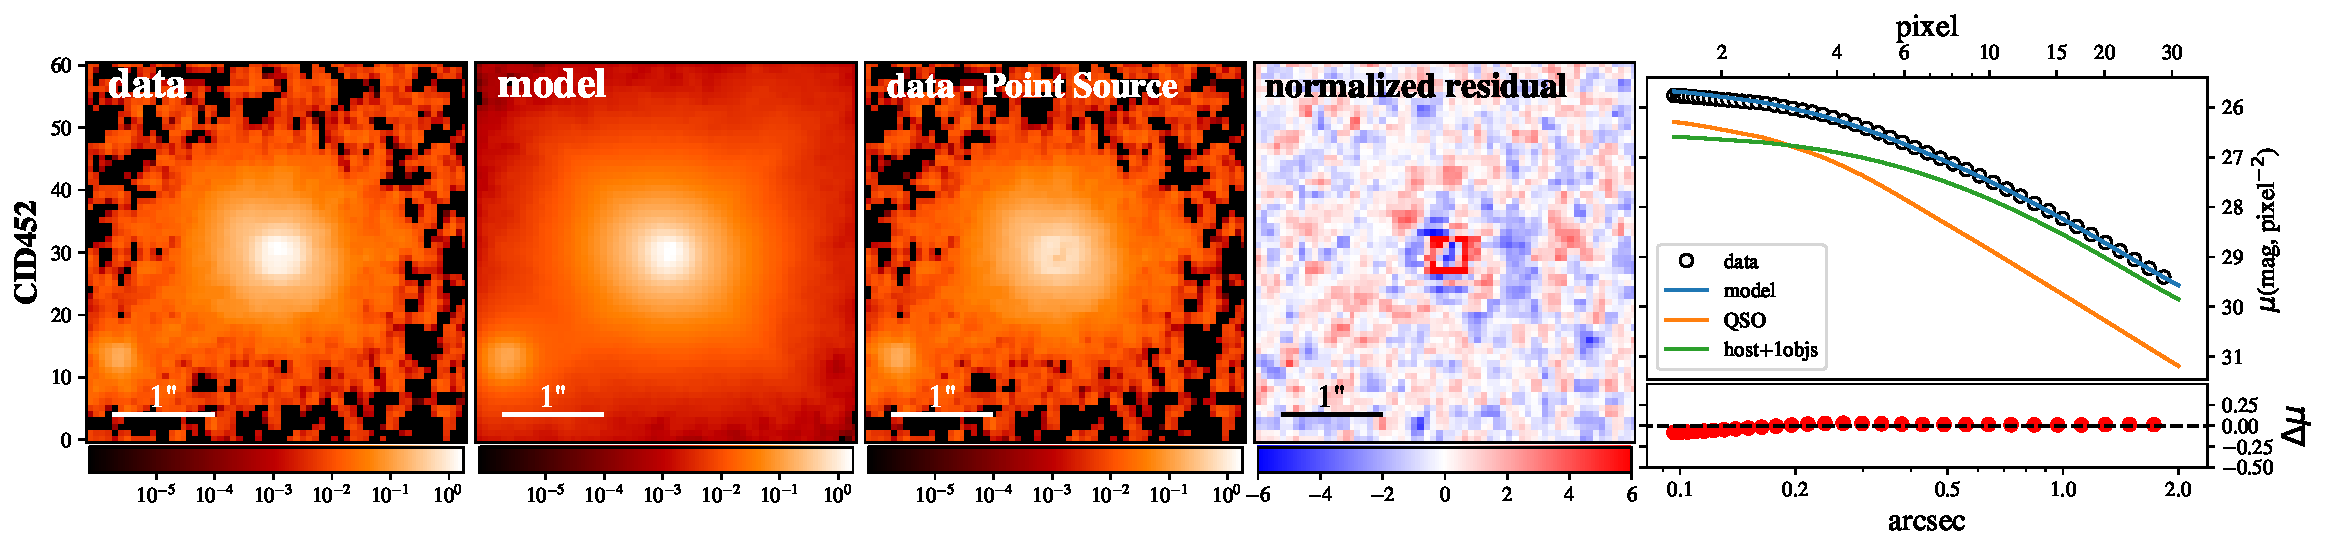
\includegraphics[height=0.25\textwidth]{fig/best_fit_CID452_SB_profile.pdf}
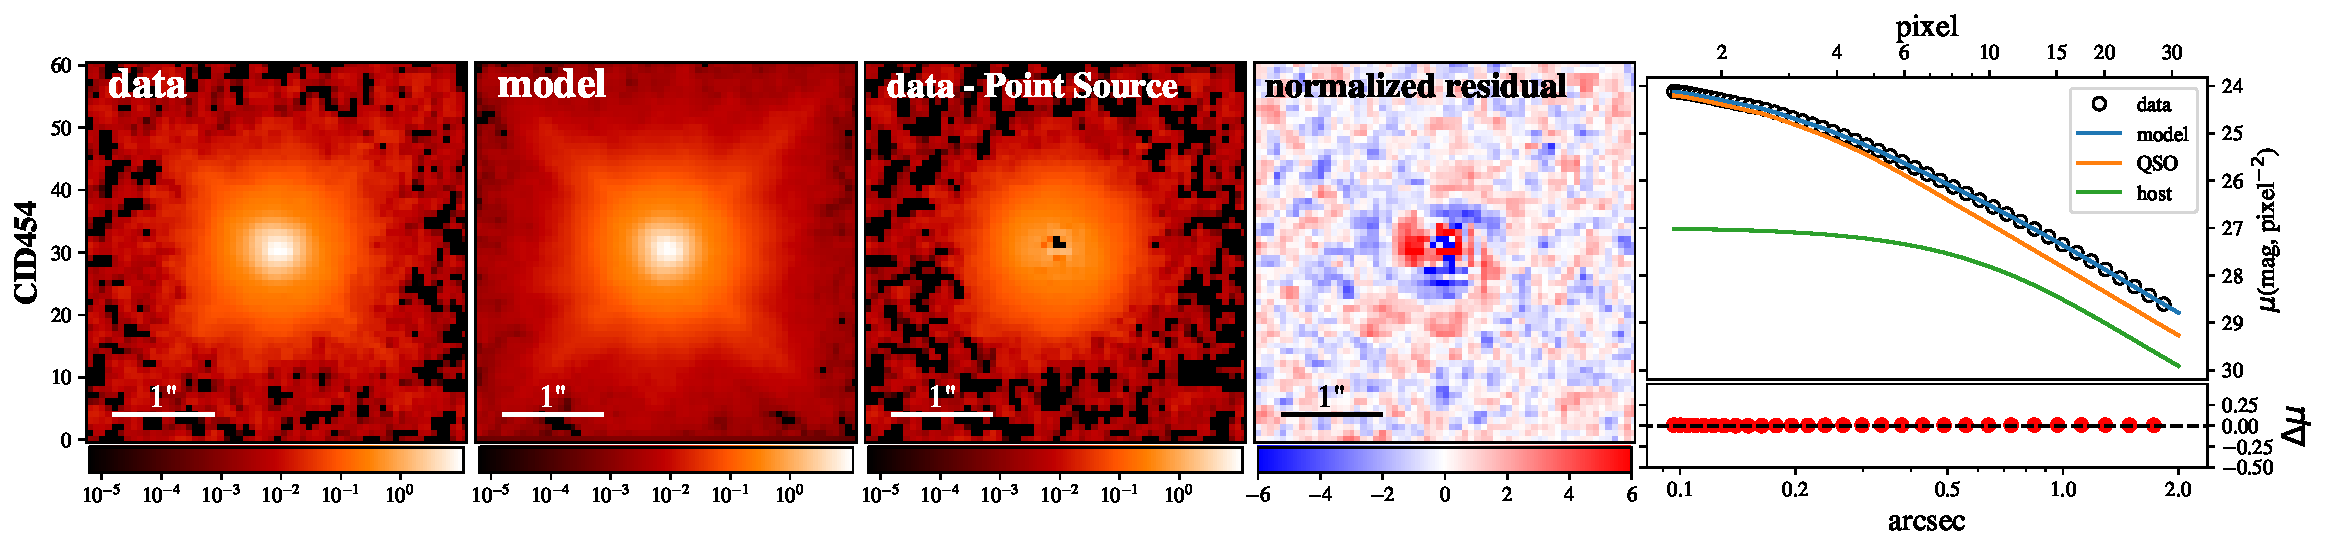
\includegraphics[height=0.25\textwidth]{fig/best_fit_CID454_SB_profile.pdf}
}
%\figurenum{1}
%\caption{Continued.}
\end{figure} 

\begin{figure*}
\centering
%\hspace{-5.5em}
{
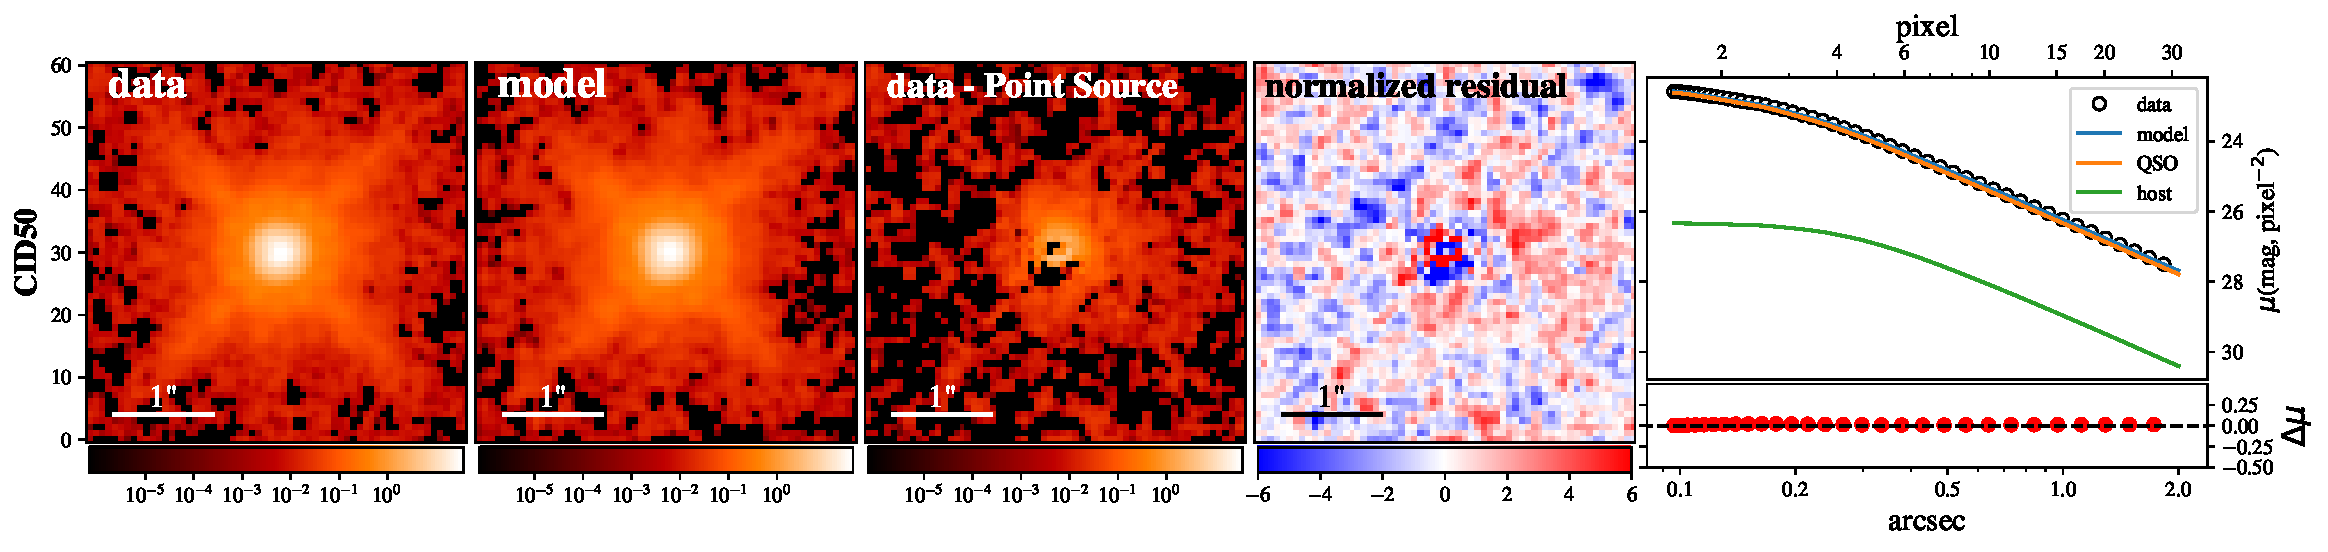
\includegraphics[height=0.25\textwidth]{fig/best_fit_CID50_SB_profile.pdf}
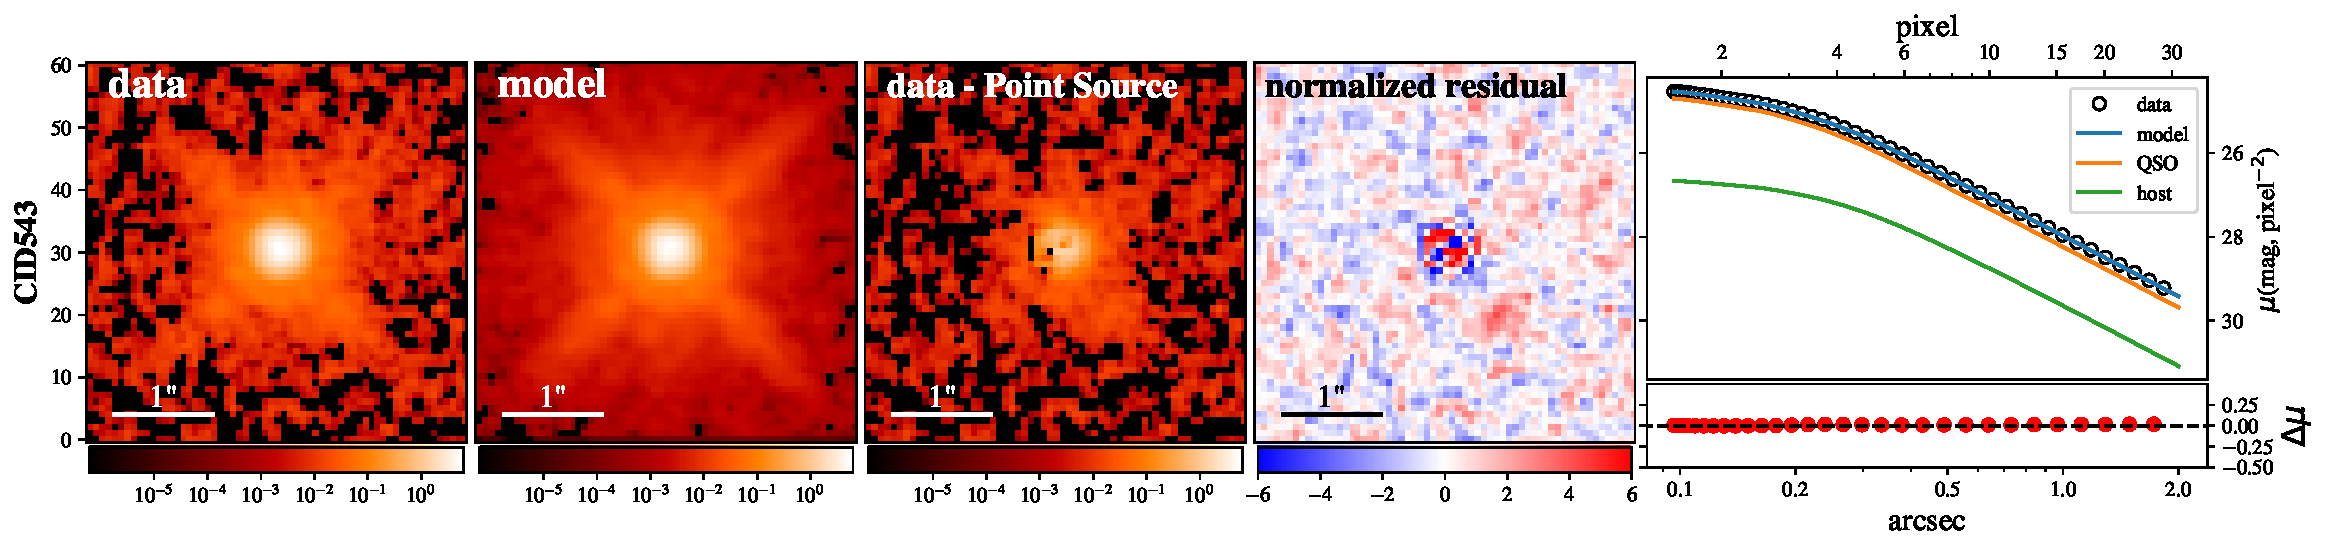
\includegraphics[height=0.25\textwidth]{fig/best_fit_CID543_SB_profile.pdf}
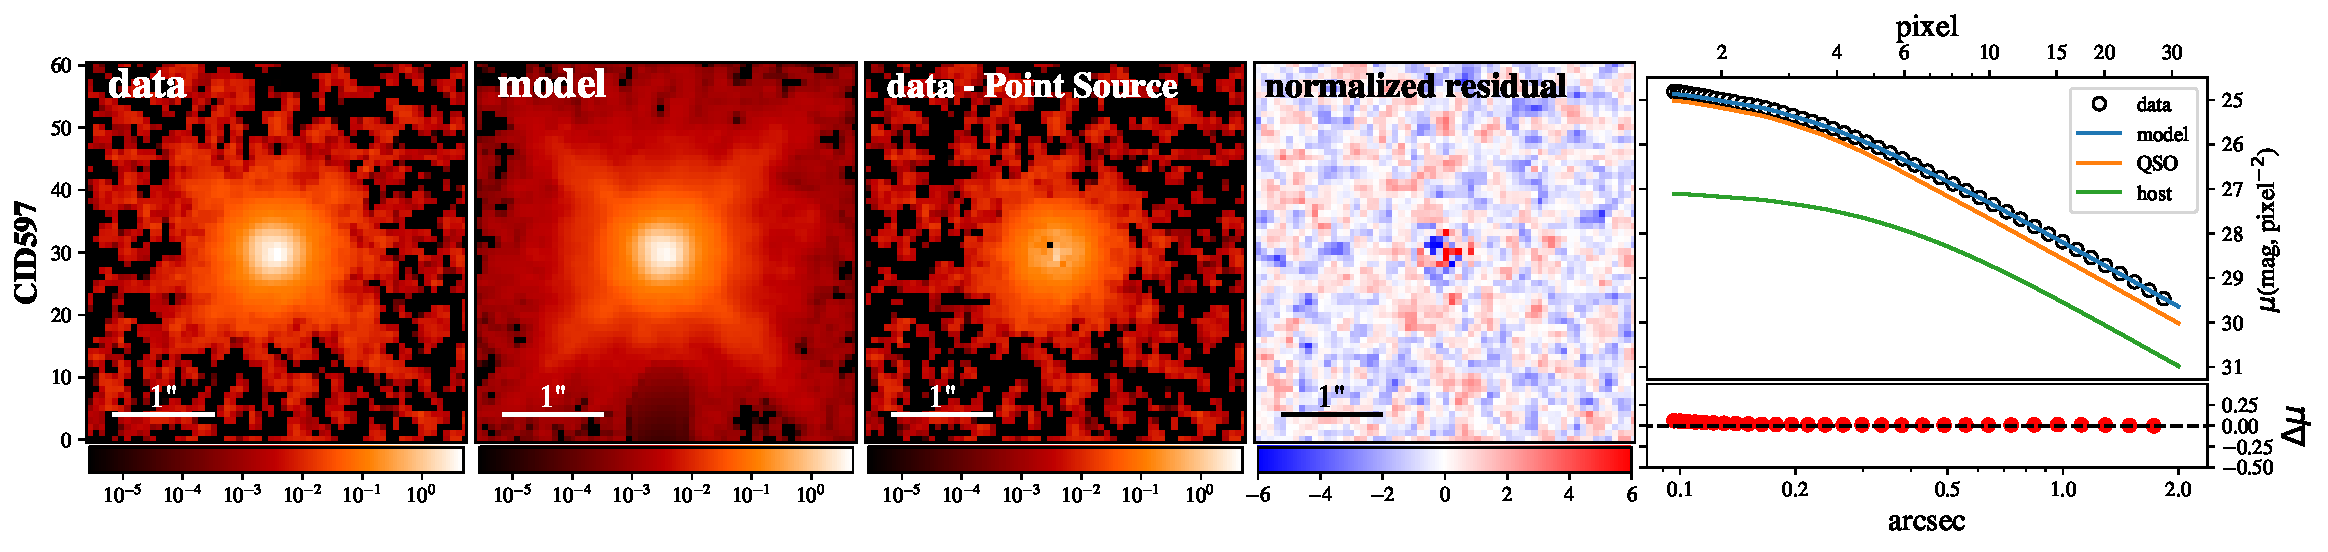
\includegraphics[height=0.25\textwidth]{fig/best_fit_CID597_SB_profile.pdf}
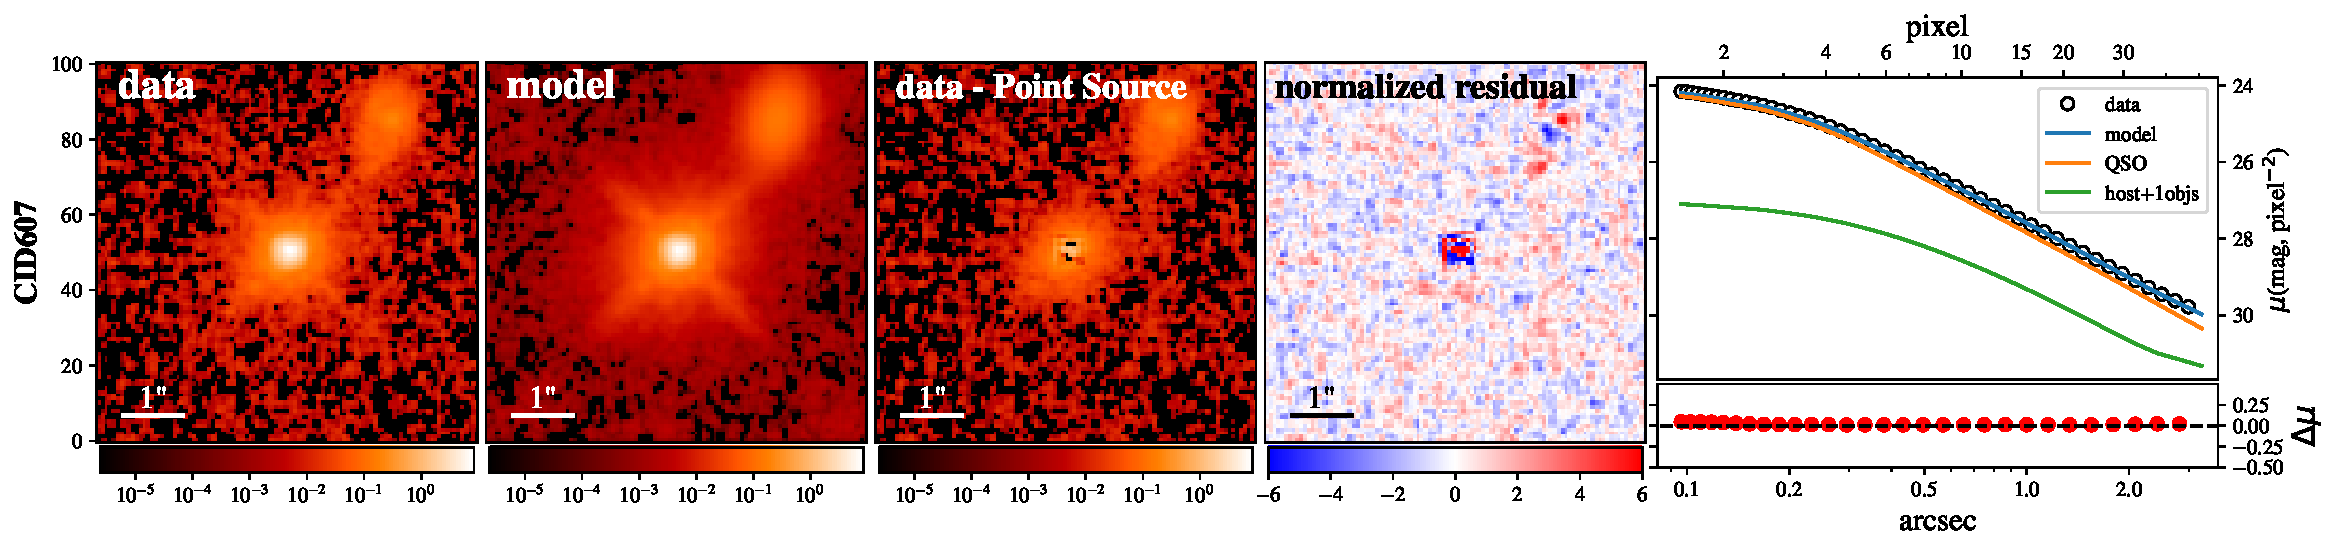
\includegraphics[height=0.25\textwidth]{fig/best_fit_CID607_SB_profile.pdf}
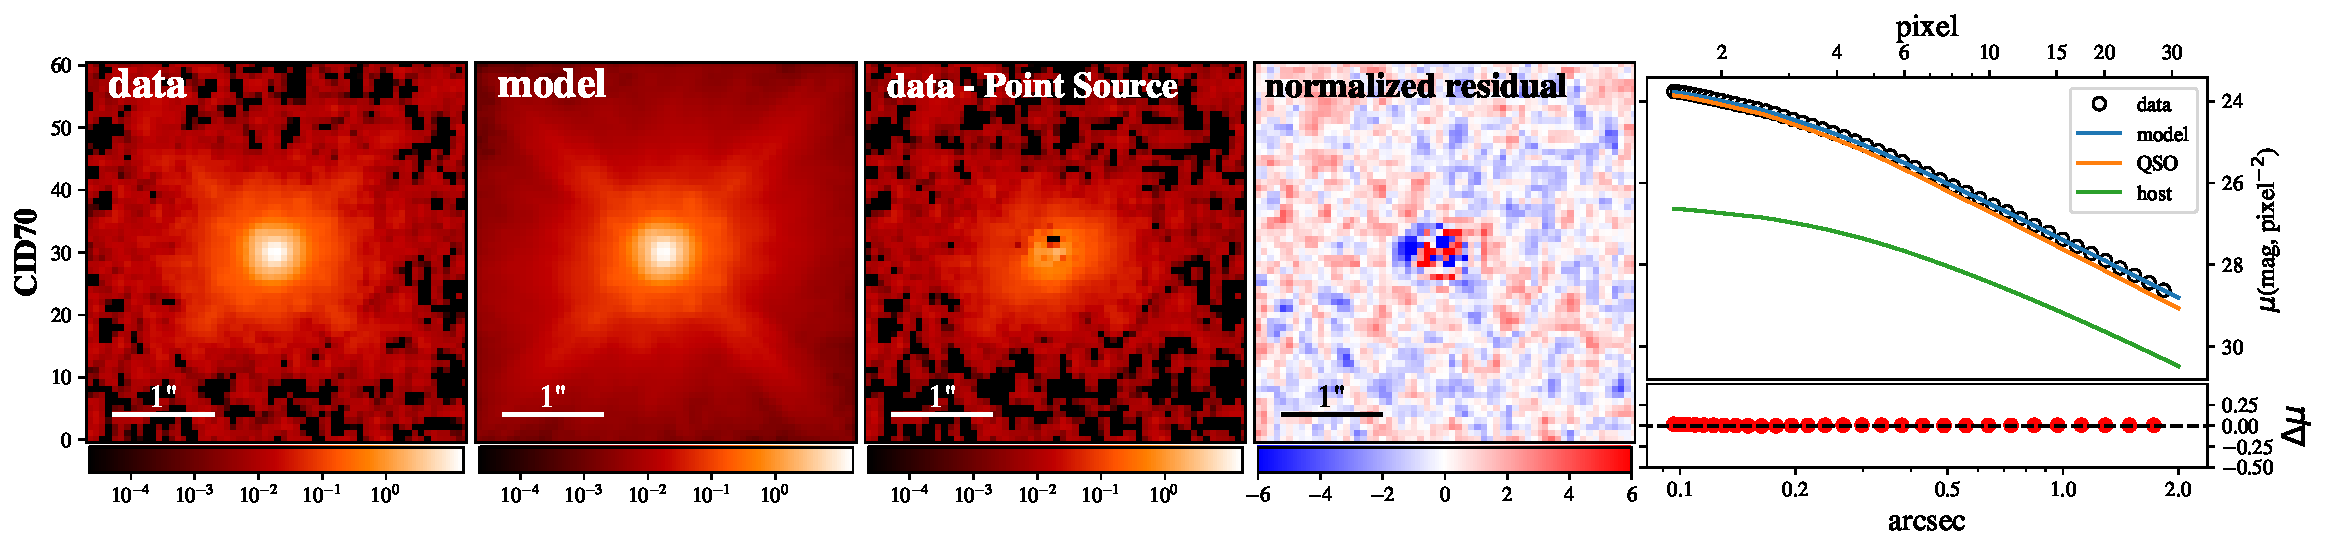
\includegraphics[height=0.25\textwidth]{fig/best_fit_CID70_SB_profile.pdf}
}
%\figurenum{1}
%\caption{Continued.}
\end{figure*} 

\begin{figure*}
\centering
%\hspace{-5.5em}
{
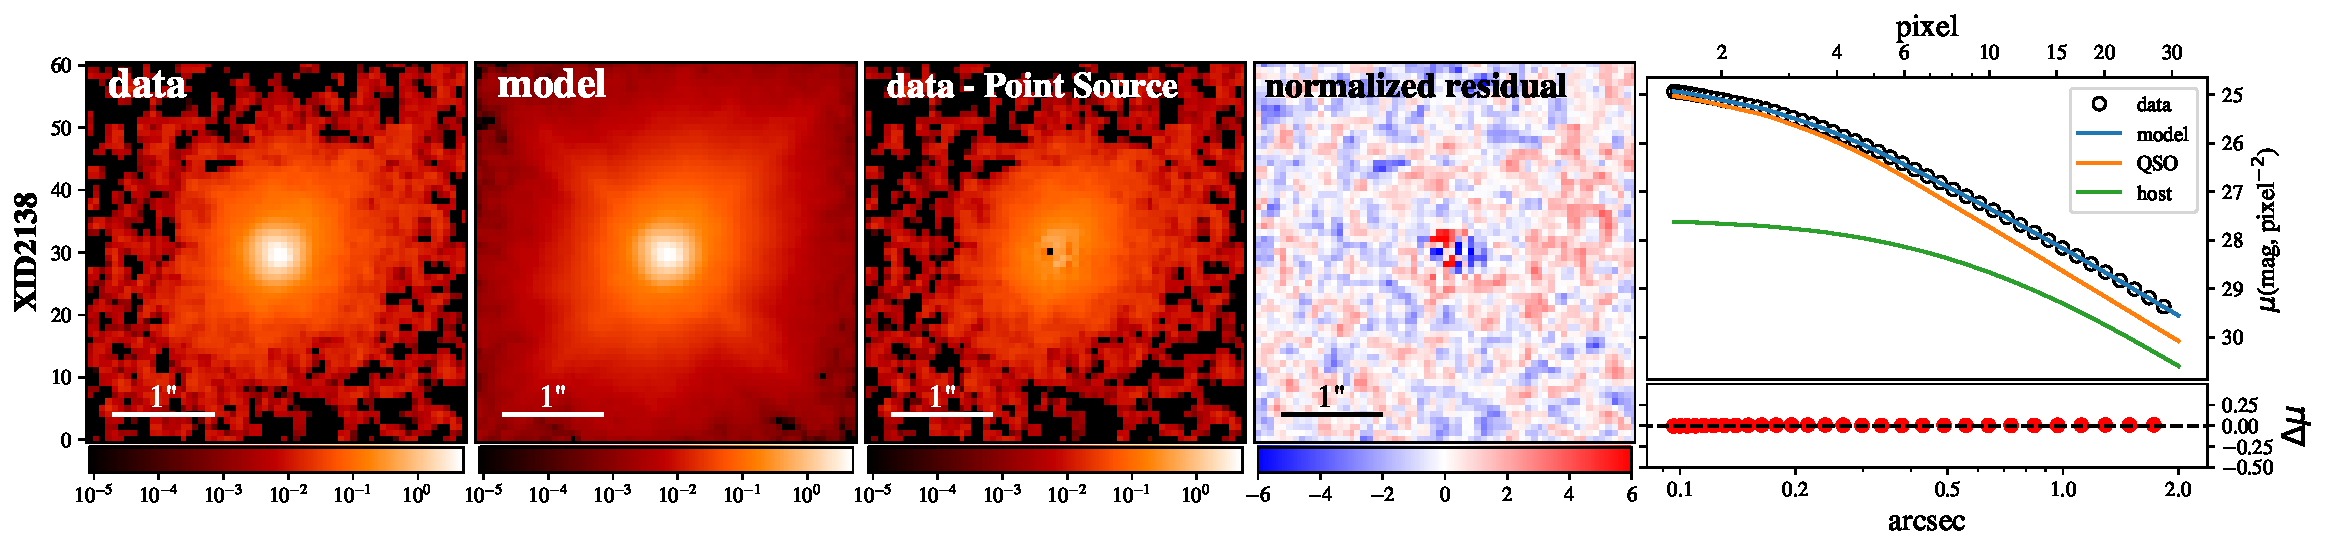
\includegraphics[height=0.25\textwidth]{fig/best_fit_XID2138_SB_profile.pdf}
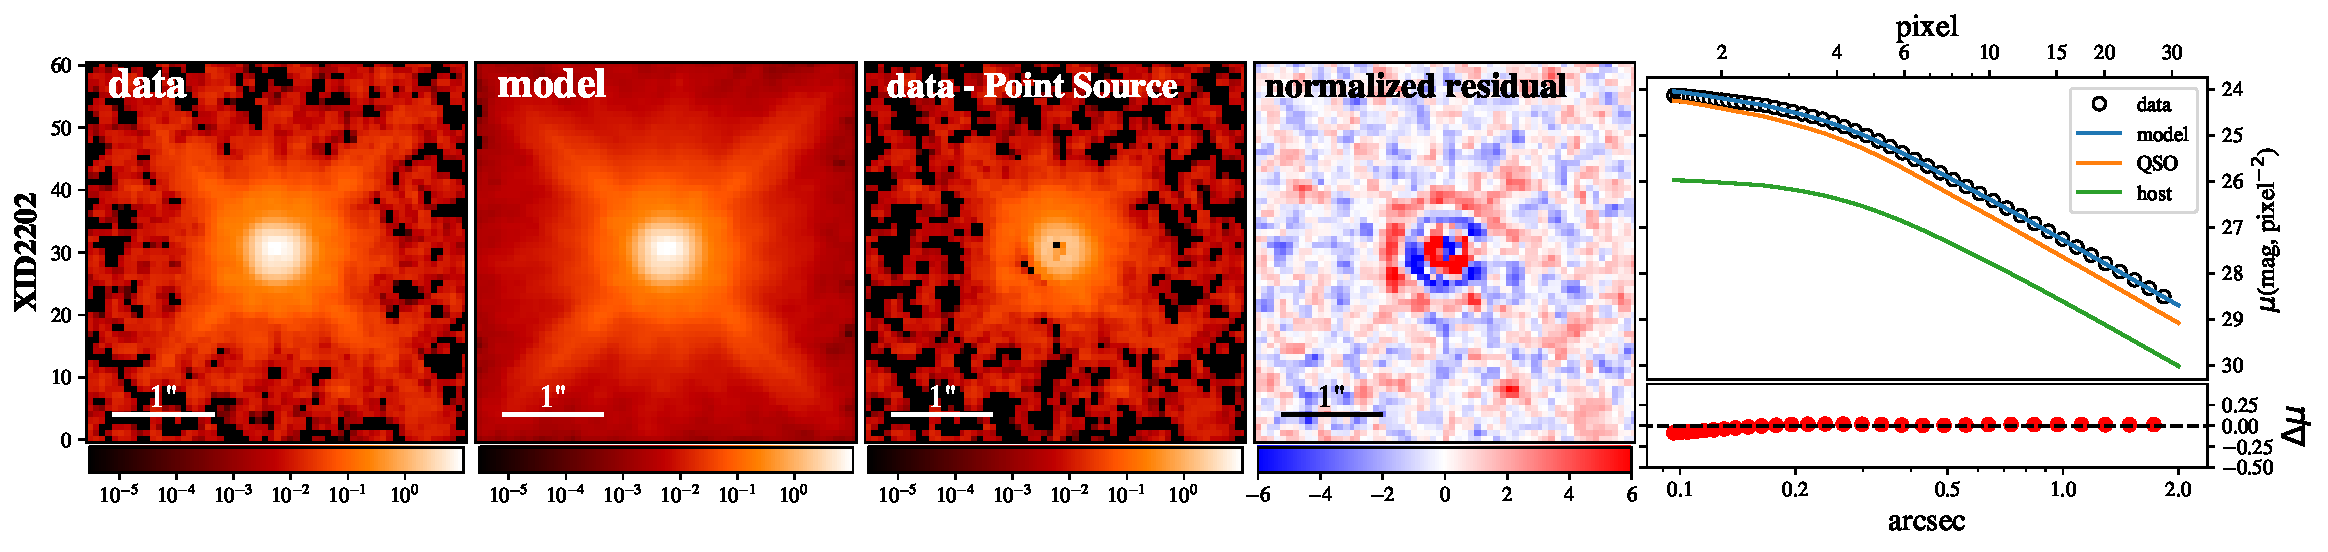
\includegraphics[height=0.25\textwidth]{fig/best_fit_XID2202_SB_profile.pdf}
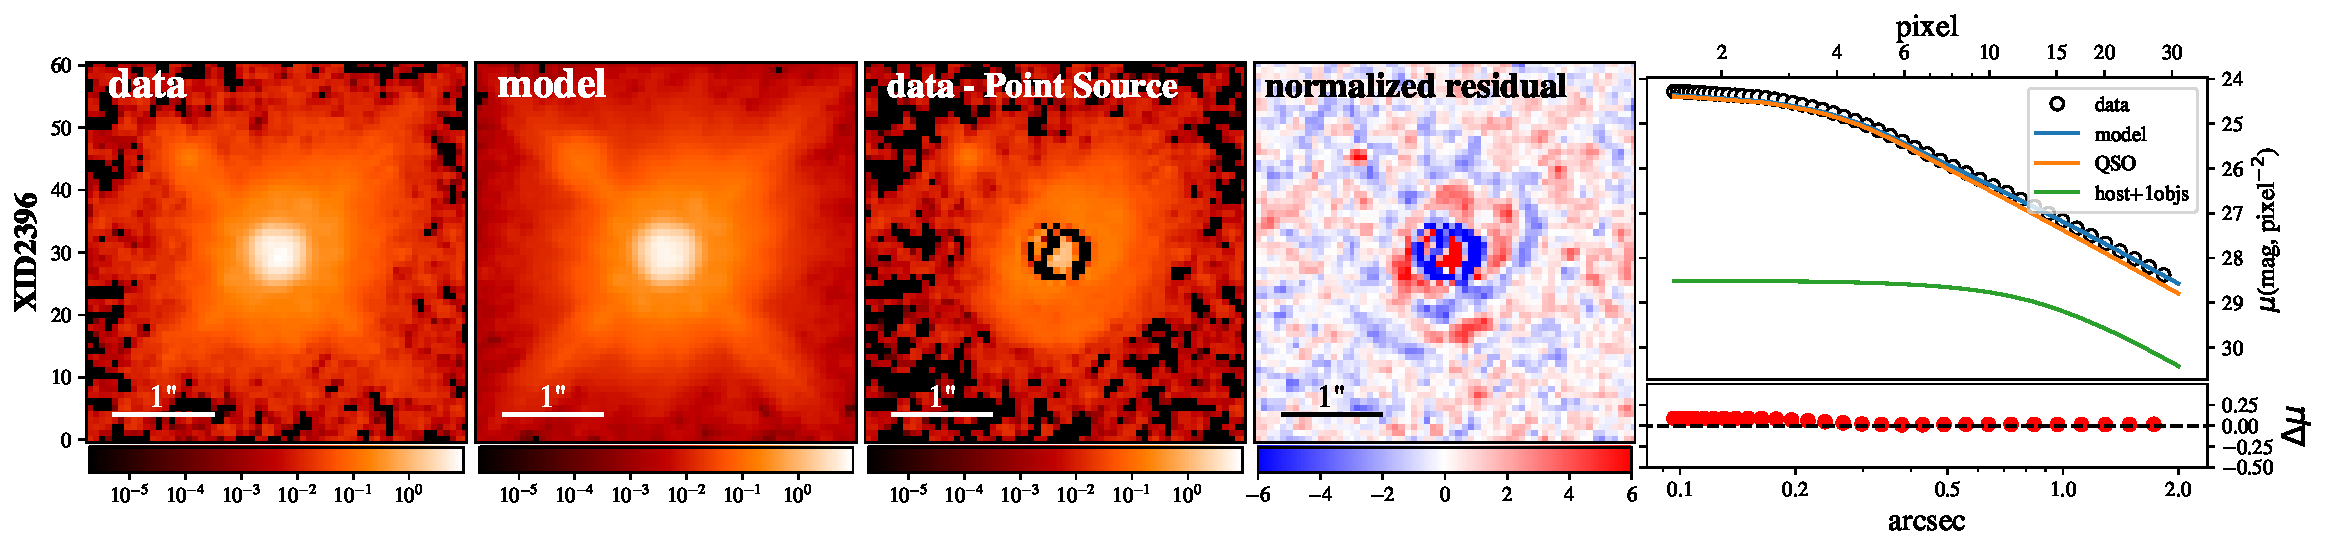
\includegraphics[height=0.25\textwidth]{fig/best_fit_XID2396_SB_profile.pdf}
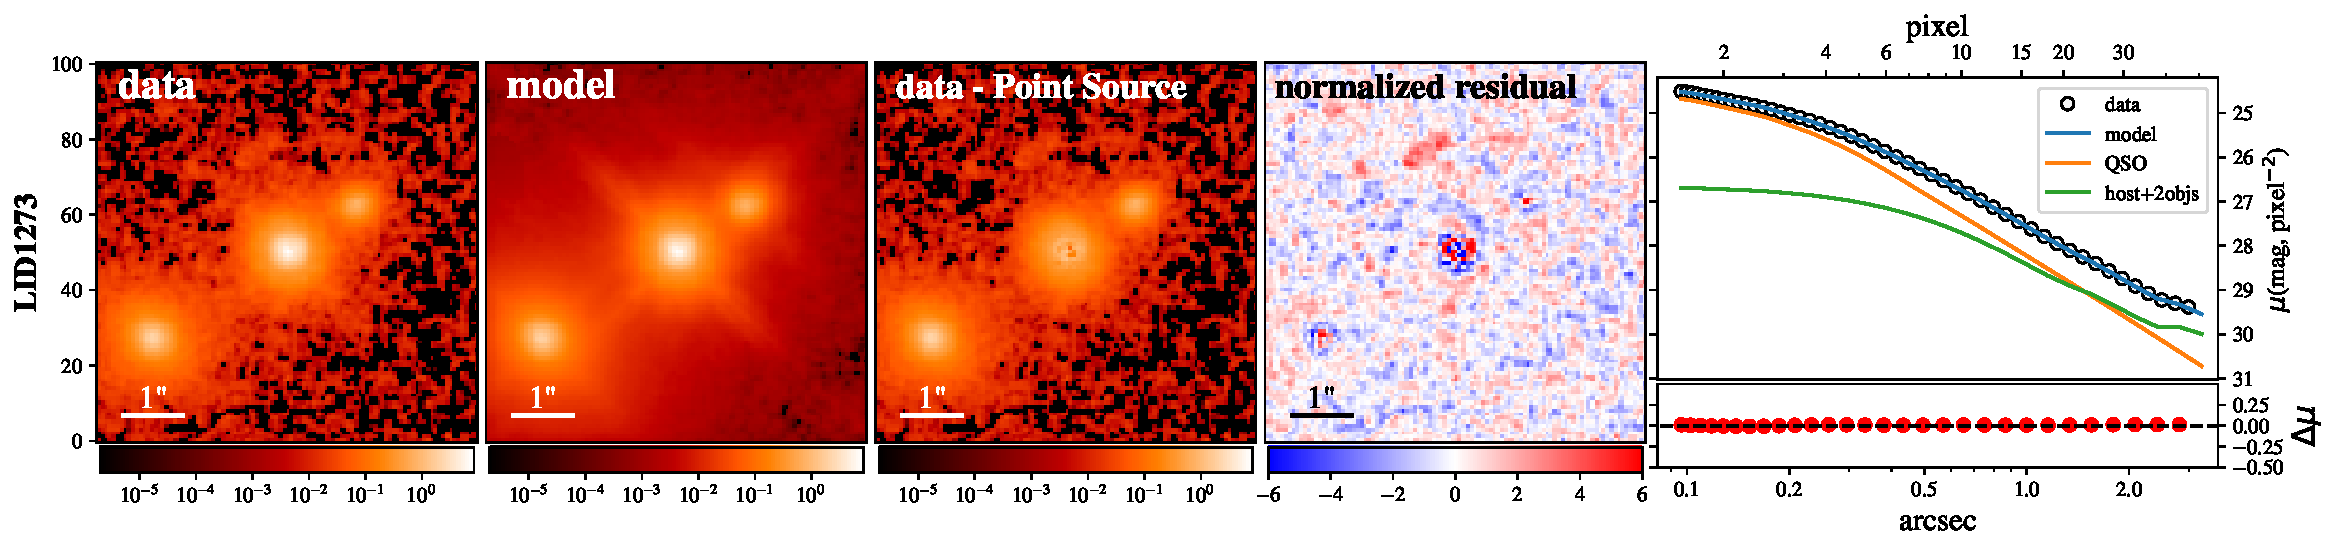
\includegraphics[height=0.25\textwidth]{fig/best_fit_LID1273_SB_profile.pdf}
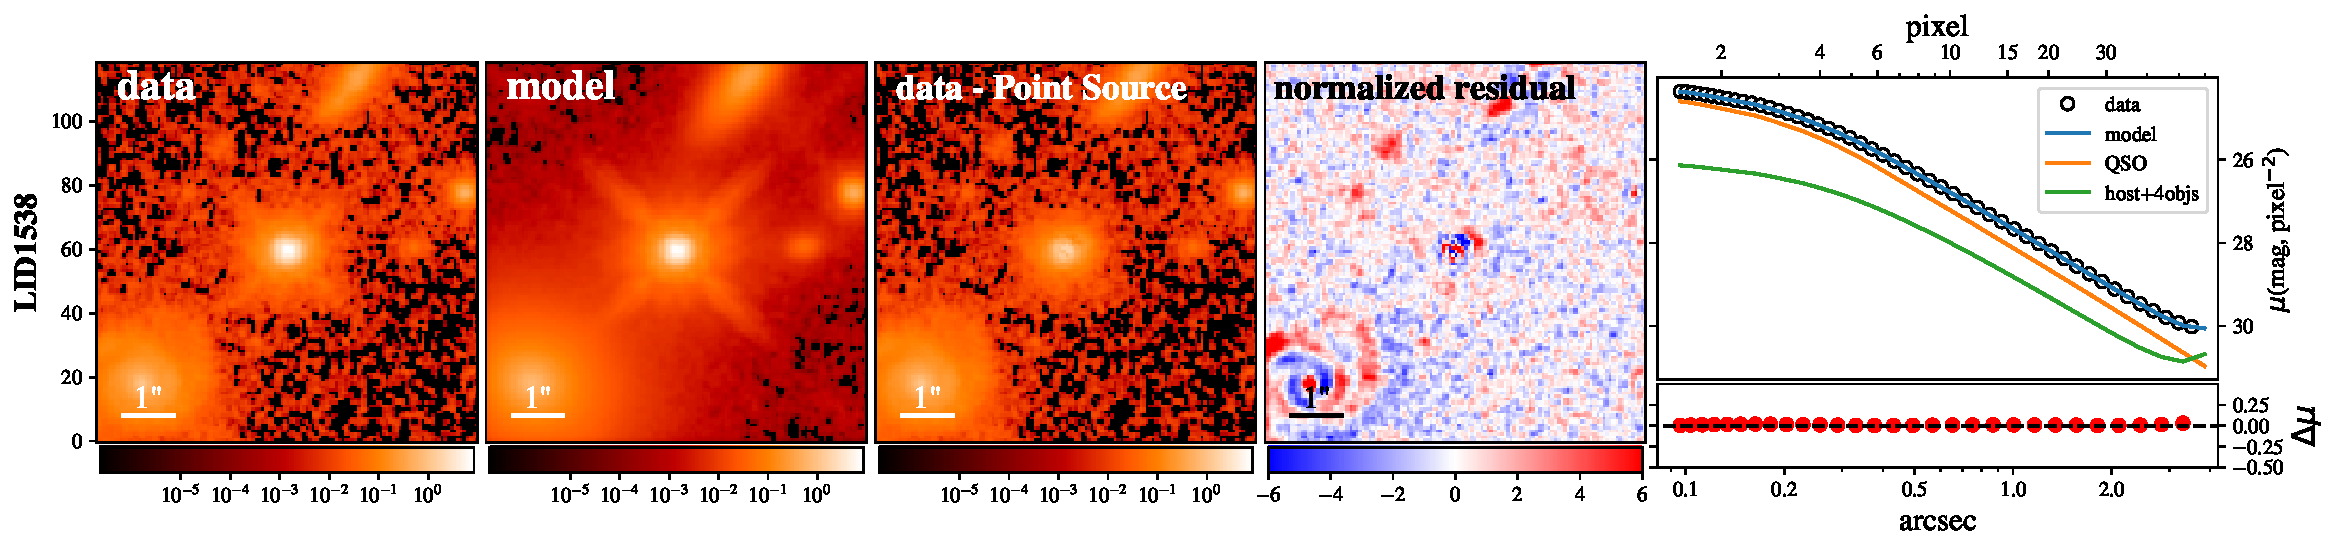
\includegraphics[height=0.25\textwidth]{fig/best_fit_LID1538_SB_profile.pdf}
}
%\figurenum{1}
%\caption{Continued.}
\end{figure*} 

\begin{figure*}
\centering
%\hspace{-5.5em}
{
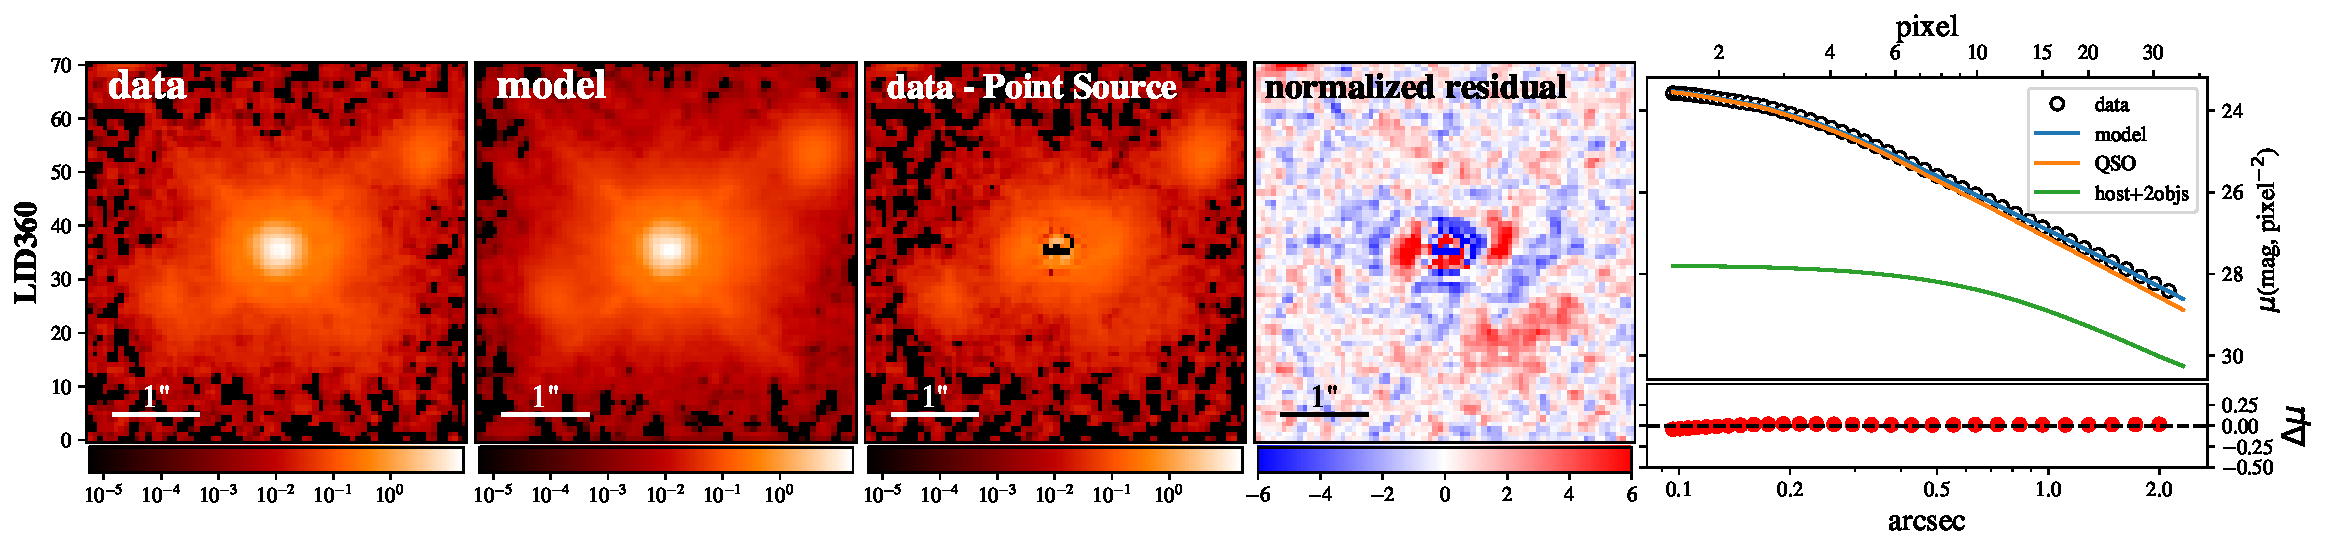
\includegraphics[height=0.25\textwidth]{fig/best_fit_LID360_SB_profile.pdf}
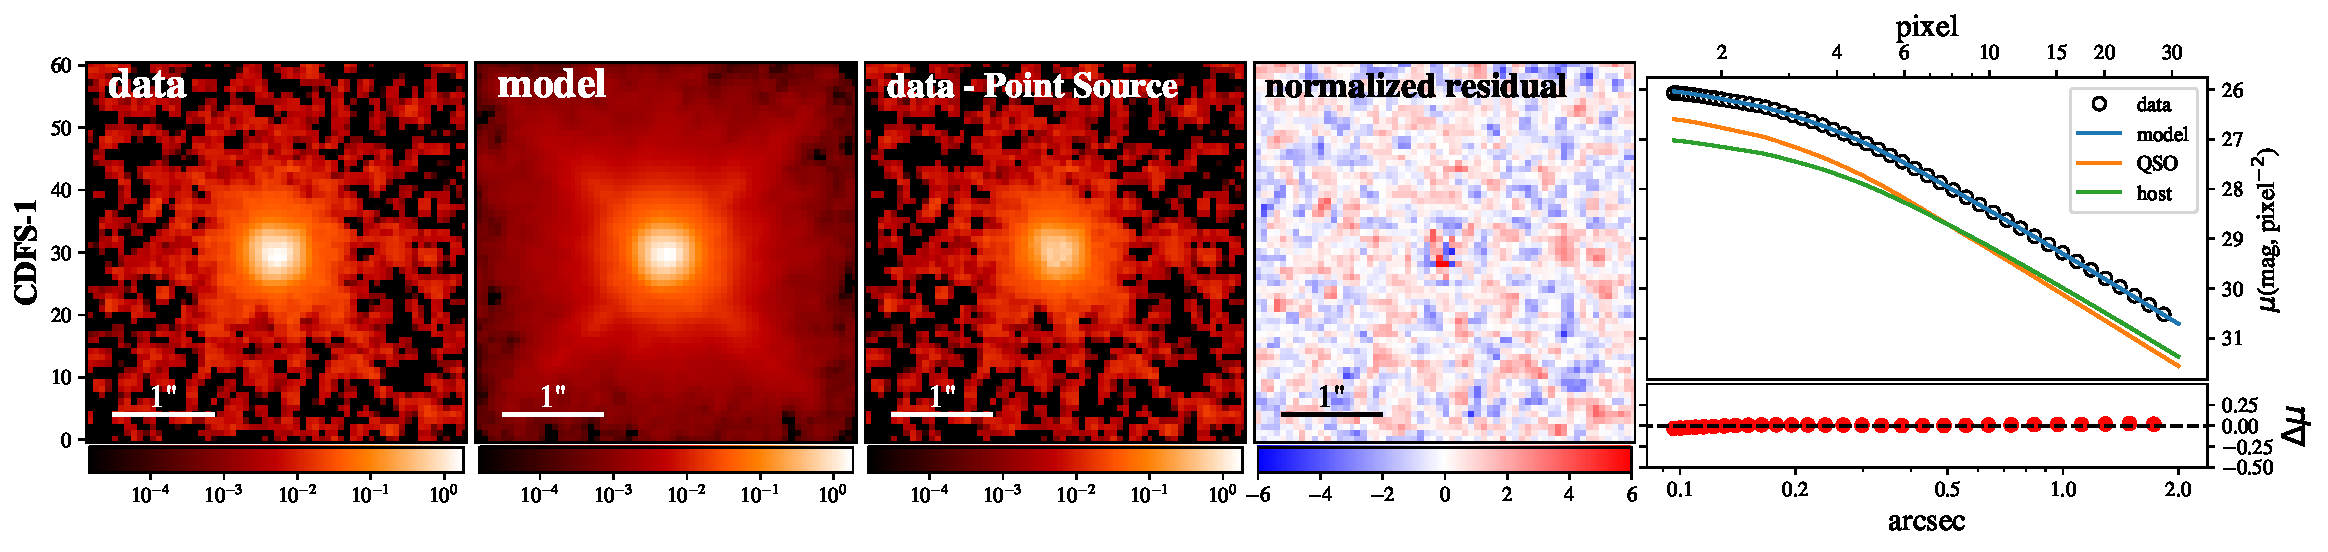
\includegraphics[height=0.25\textwidth]{fig/best_fit_CDFS-1_SB_profile.pdf}
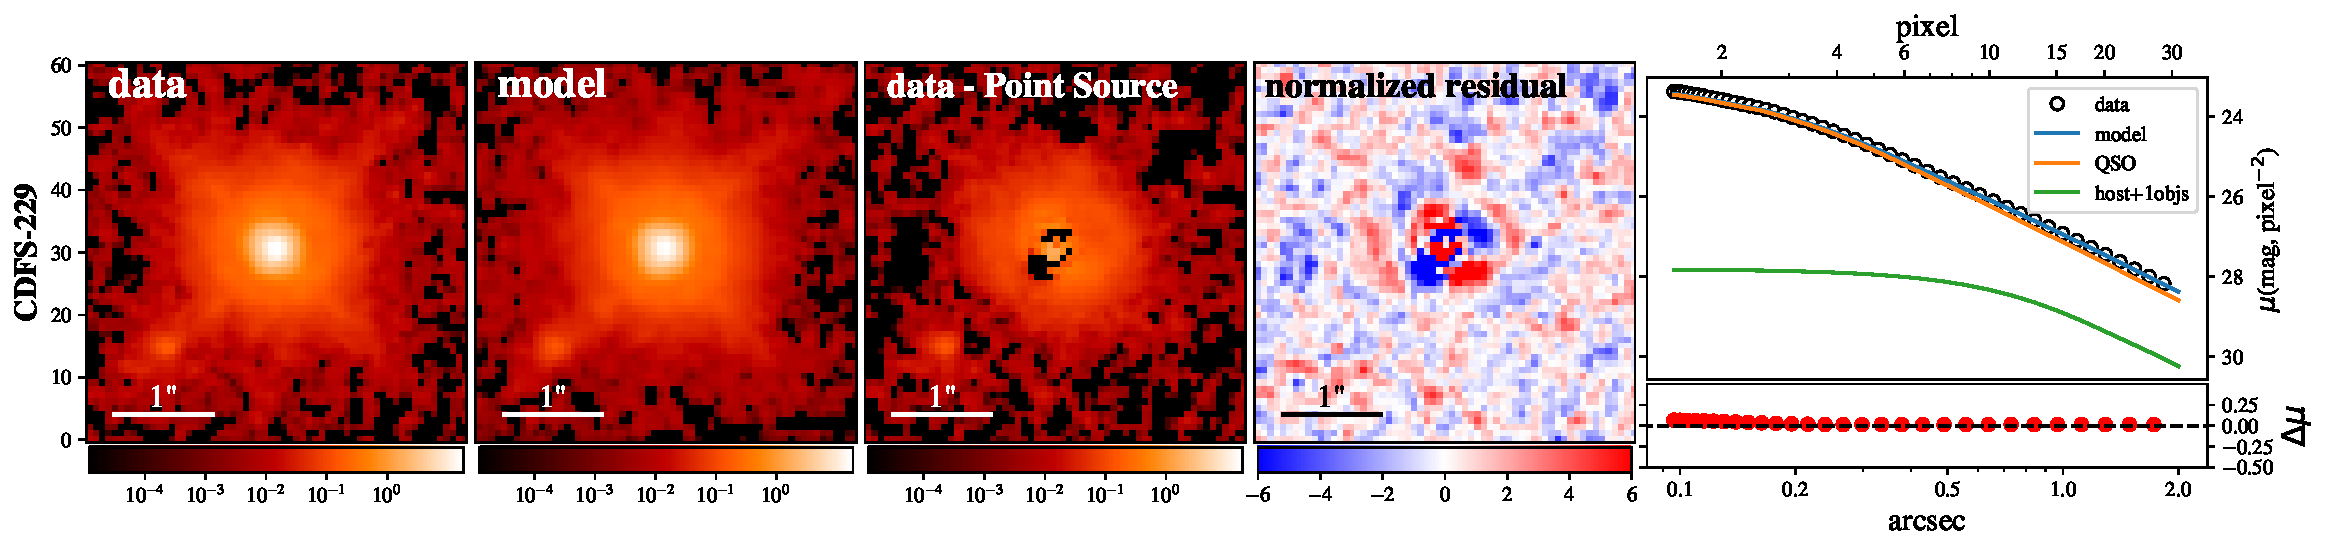
\includegraphics[height=0.25\textwidth]{fig/best_fit_CDFS-229_SB_profile.pdf}
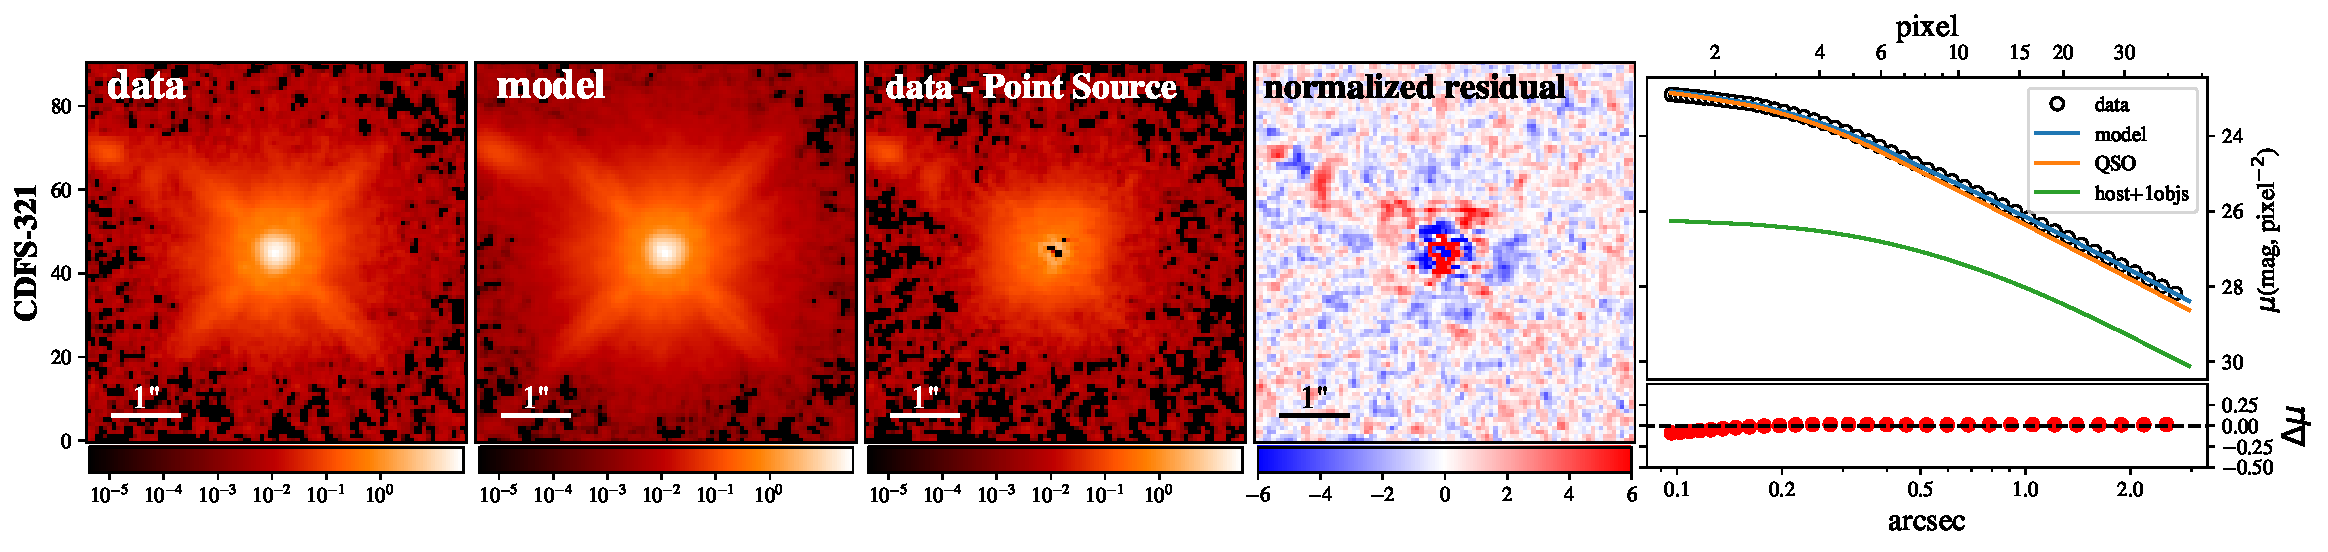
\includegraphics[height=0.25\textwidth]{fig/best_fit_CDFS-321_SB_profile.pdf}
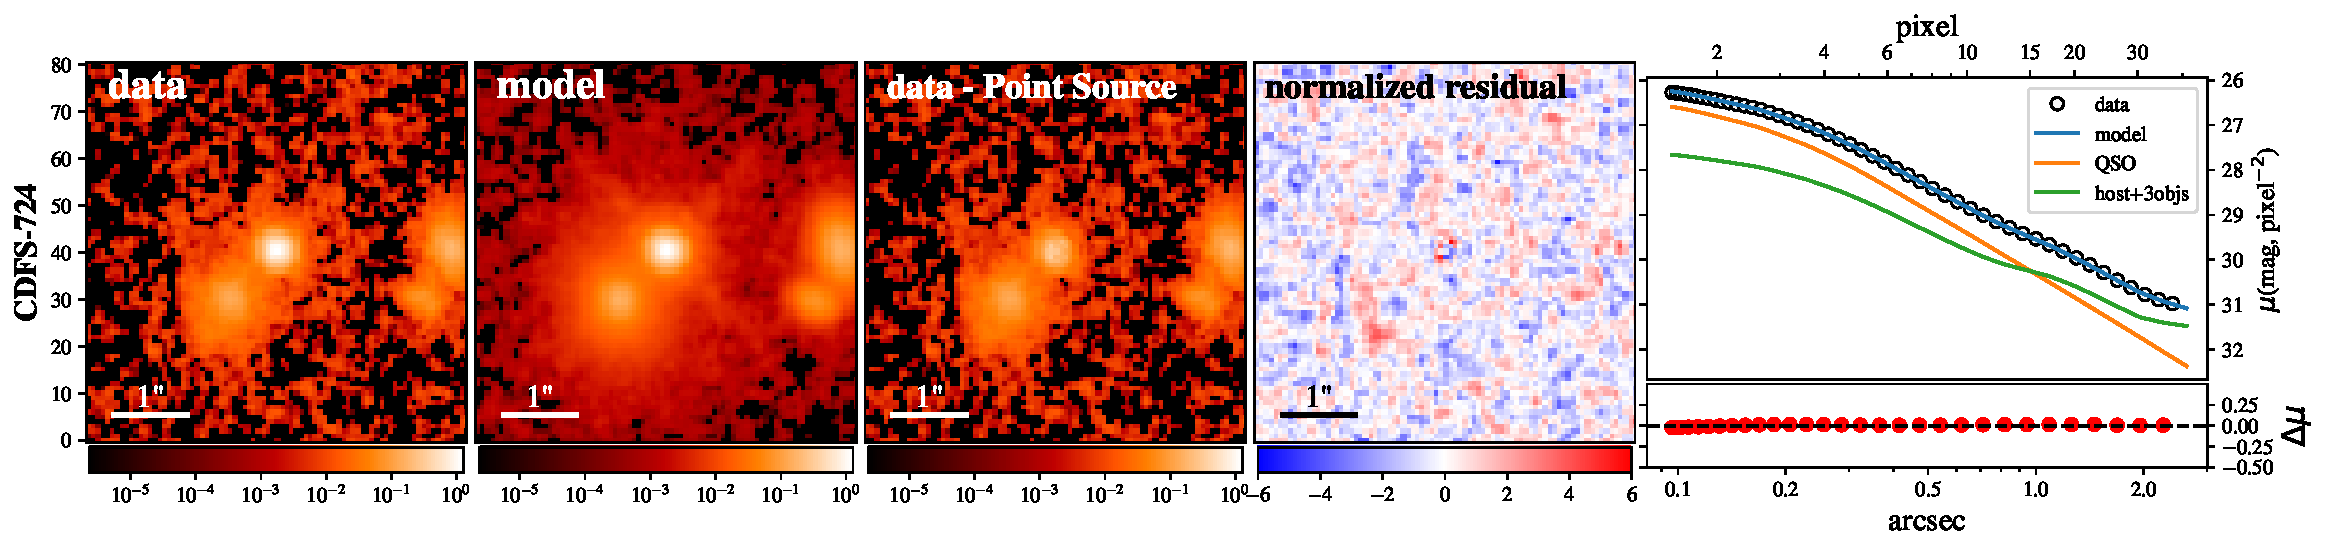
\includegraphics[height=0.25\textwidth]{fig/best_fit_CDFS-724_SB_profile.pdf}
}
%\figurenum{1}
%\caption{Continued.}
\end{figure*} 

\begin{figure*}
\centering
%\hspace{-5.5em}
{
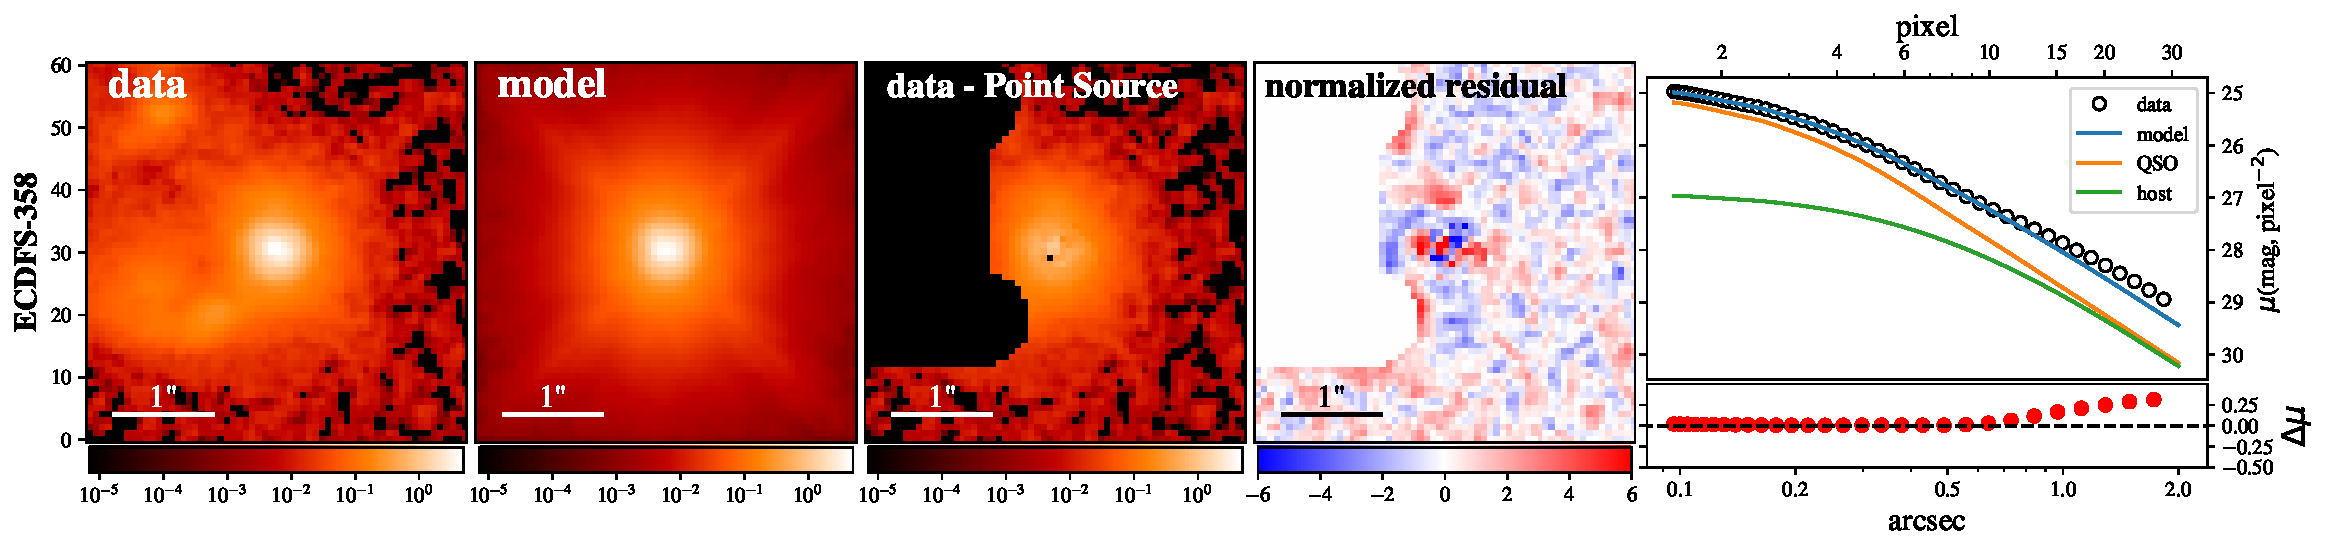
\includegraphics[height=0.25\textwidth]{fig/best_fit_ECDFS-358_SB_profile.pdf}
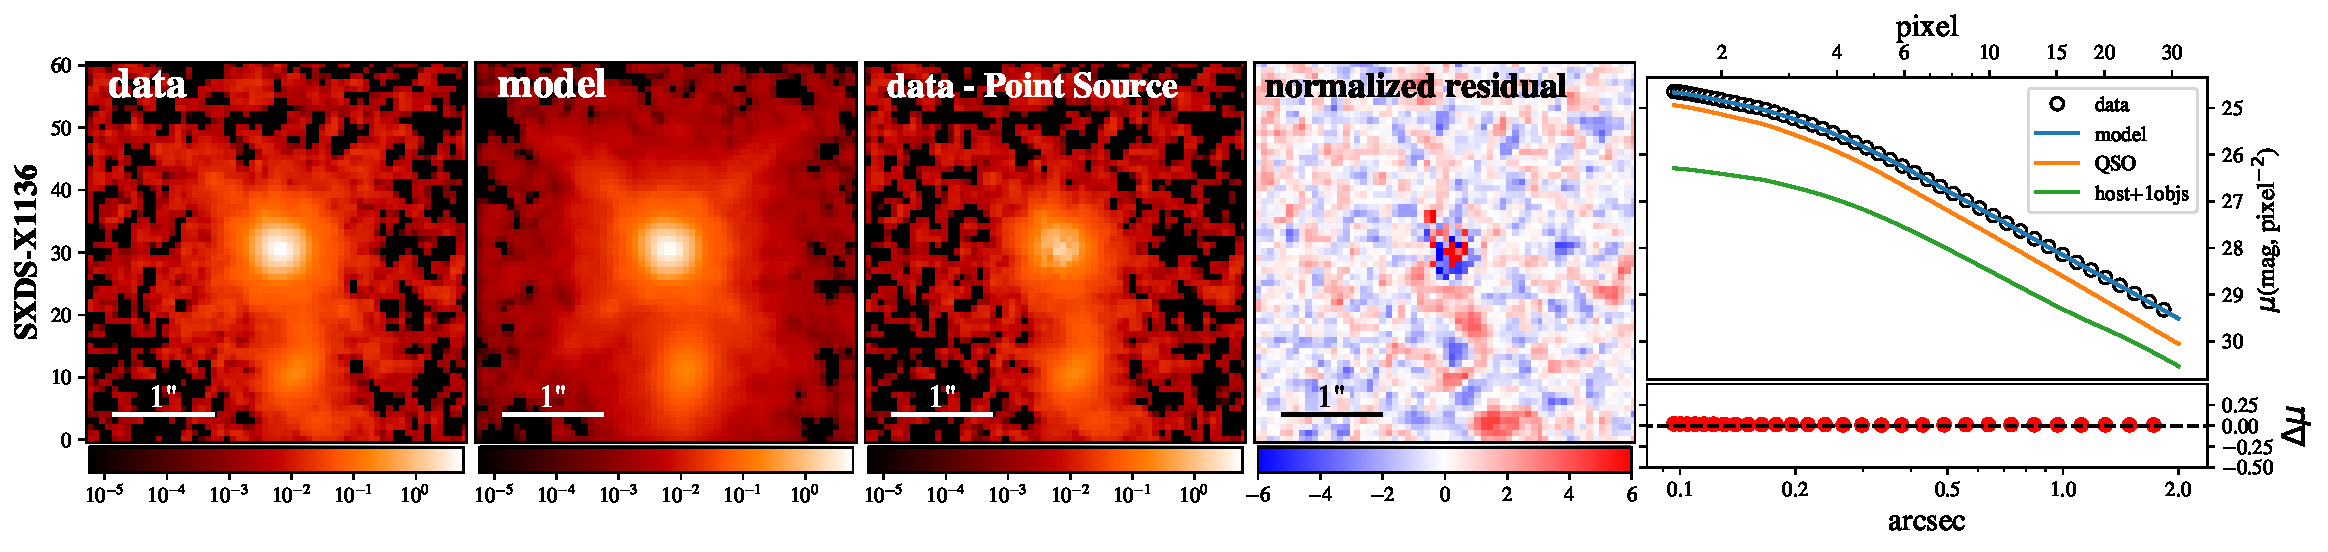
\includegraphics[height=0.25\textwidth]{fig/best_fit_SXDS-X1136_SB_profile.pdf}
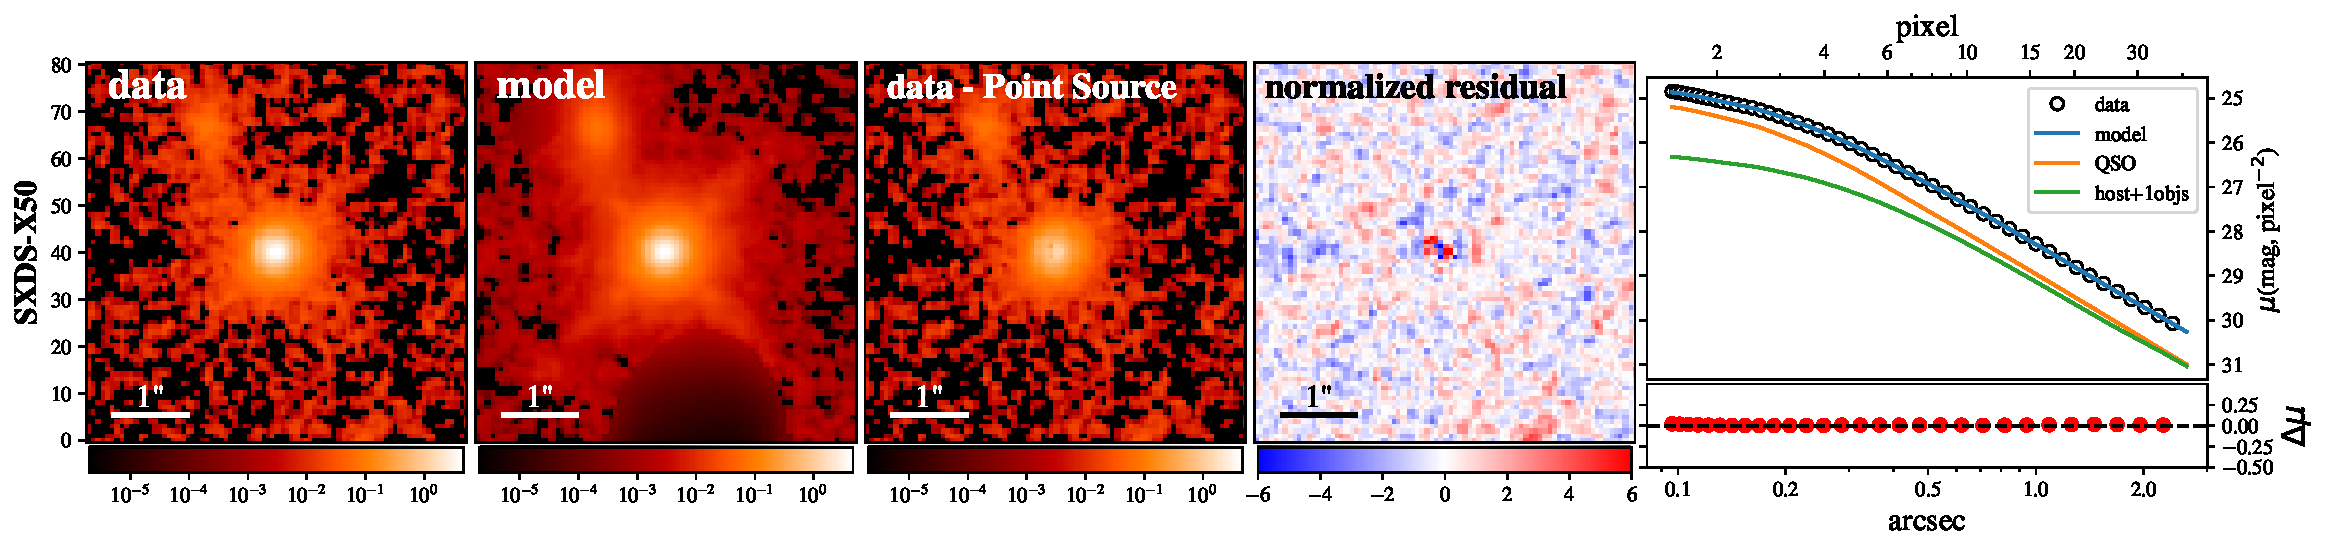
\includegraphics[height=0.25\textwidth]{fig/best_fit_SXDS-X50_SB_profile.pdf}
\includegraphics[height=0.25\textwidth]{fig/best_fit_SXDS-X717_SB_profile.pdf}
\includegraphics[height=0.25\textwidth]{fig/best_fit_SXDS-X735_SB_profile.pdf}
}
%\figurenum{1}
%\caption{Continued.}
\end{figure*} 

\begin{figure*}
\centering
%\hspace{-5.5em}
{
\includegraphics[height=0.25\textwidth]{fig/best_fit_SXDS-X763_SB_profile.pdf}
\includegraphics[height=0.25\textwidth]{fig/best_fit_SXDS-X969_SB_profile.pdf}
}
%\figurenum{1}
%\caption{Continued.}
\end{figure*} 

\clearpage
\section{B. AGN host galaxy luminosity with a correction for passive evolution}\label{sec:ml-ev}
In the passive evolution scenario, we expect the galaxy luminosity to fade over time. Thus, we transfer the \lhost\ for distant samples at today so as to compare the \mbh-\lhost\ relation to the local in the equivalent frame.
We consider this scenario following \citet{Ding2017b} by parametrizing the luminosity evolution with the functional form as
$d{\rm mag}_{\rm R}\sim~d\log(1+z)$, i.e.,
\begin{eqnarray}
\label{eq:L_relation}
\log(L_{R,0})=\log(L_{R}) - 1.48 \log (1+z).
\end{eqnarray} 
This formalism is more accurate to fit a broad range redshift comparing to a single slope as $d$mag$/dz$. We refer the interested readers to \citet[][section 5.4]{Ding2017b} for more details.

Having transferred the \lhost\ to today, we find that, as showing in Figure~\ref{fig:ML-vz}-(a), at fixed mass, the BH in the more distant universe tends to reside in less luminous hosts, which is consistent to the \mbh-\smass\ relation. We fit the offset as a function of redshift in form as Equation~\ref{eq:offset} and obtain $\gamma = 0.71 \pm 0.18$, as showing in Figure~\ref{fig:ML-vz}-(b). We further consider the selection effect using the previous approach as introduced in Section~\ref{select_eff}, and obtain $\gamma = 0.5\pm0.5$ and $\gamma = 0.6\pm0.3$, with flat and lognormal prior, respectively, as showing in Figure~\ref{fig:ML-vz}-(c), (d).

The inferred $\gamma$ here could have large systematic given the following limitations. First, the passive evolution is based on a simplified correction; after all, we are not clear exactly how the host evolves to $z=0$. Moreover, we only consider the evolution of the host galaxy and assume the \mbh\ does not change much. %Moreover, in the literature, the correlation of the \mbh-\smass\ is considered as more fundamental which would be more efficient to understand their co-evolution.

\begin{figure*}[ht]
\centering
\begin{tabular}{c c}
\subfloat[\mbh-\lhost\ relation, evolution-corrected]
{\includegraphics[height=0.5\textwidth]{fig/MBH-L_ev.pdf}}&
\subfloat[offset in  $\log($\mbh$)$ (VS. \lhost) as a function of redshift]
{\includegraphics[height=0.5\textwidth]{fig/MBH-L-vz.pdf}}\\
\subfloat[\mbh-\lhost, flat prior]
{\includegraphics[width=0.5\textwidth]{fig/ML_MC_seleff_flatprior.pdf}}&
\subfloat[\mbh-\lhost, lognormal prior]
{\includegraphics[width=0.5\textwidth]{fig/ML_MC_seleff_lognormprior.pdf}}\\
\end{tabular}
\caption{\label{fig:ML-vz} 
Same as previous figures but for \mbh-\lhost\ relation, considering the passive evolution correction for host galaxy luminosity.}
\end{figure*} 

\begin{deluxetable*}{llccccc}
\tablecolumns{7}
\tablewidth{0pt}
\tablecaption{Details of Observation} 
\tablehead{ 
\colhead{Object ID} &
\colhead{$z$} & 
\colhead{WFC3/Filter} &
\colhead{$RA$}&
\colhead{$DEC$}&
\colhead{Observing date}&
\colhead{Exposure time (s)}
\\ 
\colhead{(1)} &
\colhead{(2)} &
\colhead{(3)} &
\colhead{(4)} &
\colhead{(5)} &
\colhead{(6)} &
\colhead{(7)}
} 
\startdata
%\multicolumn{5}{c}{Sample presented in \citet{Treu+07}}\\
%\\
COSMOS-CID50 & 1.239 & F125W & 150.2080 & 2.0833 & 2017-10-23 & 2395.4\\
COSMOS-CID3570 & 1.244 & F125W & 149.6411 & 2.1076 & 2017-10-27 & 2395.4\\
COSMOS-CID597 & 1.272 & F125W & 150.5262 & 2.2449 & 2018-11-25 & 2395.4\\
COSMOS-CID607 & 1.294 & F125W & 150.6097 & 2.3231 & 2017-10-25 & 2395.4\\
COSMOS-CID543 & 1.301 & F125W & 150.4519 & 2.1448 & 2018-04-30 & 2395.4\\
COSMOS-CID452 & 1.407 & F125W & 150.0045 & 2.2371 & 2017-10-25 & 2395.4\\
COSMOS-CID1281 & 1.445 & F140W & 150.4160 & 2.5258 & 2018-11-26 & 2395.4\\
COSMOS-CID454 & 1.478 & F140W & 149.8681 & 2.3307 & 2018-02-26 & 2395.4\\
COSMOS-CID206 & 1.483 & F140W & 149.8371 & 2.0088 & 2017-10-23 & 2395.4\\
COSMOS-XID2202 & 1.516 & F140W & 150.6530 & 1.9969 & 2017-11-05 & 2395.4\\
COSMOS-LID1538 & 1.527 & F140W & 150.6215 & 2.1588 & 2018-05-01 & 2395.4\\
COSMOS-CID3242 & 1.532 & F140W & 149.7113 & 2.1452 & 2017-10-26 & 2395.4\\
COSMOS-XID2138 & 1.551 & F140W & 149.7036 & 2.5781 & 2017-11-01 & 2395.4\\
COSMOS-CID1174 & 1.552 & F140W & 150.2789 & 1.9595 & 2017-10-26 & 2395.4\\
COSMOS-CID216 & 1.567 & F140W & 149.7918 & 1.8729 & 2017-10-23 & 2395.4\\
COSMOS-LID360 & 1.579 & F140W & 150.1251 & 2.8617 & 2017-10-30 & 2395.4\\
COSMOS-XID2396 & 1.600 & F140W & 149.4779 & 2.6425 & 2017-11-12& 2395.4\\
COSMOS-LID1273 & 1.617 & F140W & 150.0565 & 1.6275 & 2017-10-31 & 2395.4\\
COSMOS-CID237 & 1.618 & F140W & 149.9916 & 1.7243 & 2018-06-03 & 2395.4\\
COSMOS-CID255\footnoteref{note1} & 1.664 & F140W & 150.1017 & 1.8483 & 2019-03-16 & 2395.4\\
COSMOS-CID70 & 1.667 & F140W & 150.4051 & 2.2701 & 2017-10-27 & 2395.4\\
CDFS-229 & 1.326 & F125W & 53.0680 & -27.6580 & 2018-04-04 & 2395.4\\ 
CDFS-724 & 1.337 & F125W & 53.2870 & -27.6940 & 2018-04-05 & 2395.4\\ 
CDFS-321 & 1.570 & F140W & 53.0486 & -27.6239 & 2018-08-18& 2395.4\\ 
ECDFS-358 & 1.626 & F140W & 53.0850 & -28.0370 & 2018-02-09& 2395.4\\ 
CDFS-1 & 1.630 & F140W & 52.8990 & -27.8600 & 2018-04-03 & 2395.4\\
SXDS-X717 & 1.276 & F125W & 34.5400 & -5.0334 & 2018-07-02 & 2395.4\\ 
SXDS-X1136 & 1.325 & F125W & 34.8925 & -5.1498 & 2018-01-29& 2395.4\\ 
SXDS-X50 & 1.411 & F125W & 34.0267 & -5.0602 & 2018-03-01& 2395.4\\ 
SXDS-X763 & 1.412 & F125W & 34.5849 & -4.7864 & 2018-07-03 & 2395.4\\ 
SXDS-X735 & 1.447 & F140W & 34.5581 & -4.8781 & 2017-11-14 & 2395.4\\ 
SXDS-X969 & 1.585 & F140W & 34.7594 & -5.4291 & 2018-07-02 & 2395.4\\ 
\enddata
\label{tab:objlist}
\tablecomments{
Column 1: Object field and ID.
Column 2: Spectroscopic redshift.
Column 3: WFC3 filter. Note that the targets from the COSMOS and (E)-CDF-S fields also have ACS imaging.
Column 4 and 5: J2000 $RA$ and $DEC$ coordinates.
Column 6: The observing start date.
Column 7: Total exposure time.
}
\end{deluxetable*}

\begin{deluxetable*}{ccccccc}
\tablecolumns{7}
\tablewidth{0pt}
\tablecaption{Host inference of CID1174} 
\tablehead{ 
\colhead{PSF rank} &
\colhead{total $\chi ^2$} & 
\colhead{weights $w_i$} &
\colhead{host flux (counts)} &
\colhead{host flux ratio}&
\colhead{\Reff (arcsec)}&
\colhead{\sersic\ $n$}
 \\ 
\colhead{(1)} &
\colhead{(2)} &
\colhead{(3)} &
\colhead{(4)} &
\colhead{(5)} &
\colhead{(6)} &
\colhead{(7)} 
} 
\startdata
%\multicolumn{5}{c}{Sample presented in \citet{Treu+07}}\\
%\\
1 & $8584.429$ & $1.000$ & $82.2$ & $35\%$ & $0\farcs{}345$ & $1.1$ \\
2 & $8646.711$ & $0.920$ & $99.1$ & $42\%$ & $0\farcs{}298$ & $1.9$ \\
3 & $8816.947$ & $0.734$ & $76.7$ & $33\%$ & $0\farcs{}365$ & $1.1$ \\
4 & $9304.841$ & $0.383$ & $128.6$ & $55\%$ & $0\farcs{}231$ & $2.8$ \\
5 & $9652.575$ & $0.241$ & $187.5$ & $79\%$ & $0\farcs{}116$ & $6.2$ \\
6 & $9917.101$ & $0.170$ & $100.2$ & $42\%$ & $0\farcs{}287$ & $2.1$ \\
7 & $10018.324$ & $0.148$ & $75.1$ & $32\%$ & $0\farcs{}365$ & $1.2$ \\
8 & $10087.456$ & $0.135$ & $79.8$ & $34\%$ & $0\farcs{}358$ & $1.2$ \\
\hline\\
Weighted value & & & $97.322\pm28.336$ & $42\%\pm12\%$& $0\farcs{}309\pm0\farcs{}065$  & $1.9\pm1.3$  \\
\enddata
\label{tab:weight_CID1174}
\tablecomments{
Column~1: Rank of the PSF from the library.
Column~2: Total $\chi ^2$ for the corresponding PSF.
Column~3: Weights for the inference.
Column~4-7: Fitted value for the host flux, host/total flux ratio, effective radius, and \sersic\ index.
For this sample, the inflation parameter $\alpha$ calculated by Equation~\ref{eq:alpha} is 16.671.
}
\end{deluxetable*}


\begin{deluxetable*}
{@{\extracolsep{4pt}}lcccccccc}   % need for the gap between the clines.
\tablecolumns{9}
\tablewidth{0pt}
\tablecaption{Inferred BH properties for the 32 systems} 
\tablehead
{ 
\colhead{Target ID}&
  \multicolumn{4}{c}{using emission line \halpha}&
  \multicolumn{4}{c}{using emission line \hbeta} \\
  \cline{2-5}  \cline{6-9} \\
\colhead{}& 
\colhead{FWHM}& \colhead{$\log( \rm L _{H\alpha}$)}& \colhead{$\log$\mbh}& Eddington ratio &
\colhead{FWHM(5100)}& \colhead{$\log( \rm L _{\lambda5100})$}& \colhead{$\log$\mbh}& Eddington ratio \\
\colhead{}& 
\colhead{(\kms)}& \colhead{(${\rm erg~s^{-1}}$)}& 
\colhead{(M$_{\odot}$)}& (log$\lambda$)&
\colhead{(\kms)}& 
\colhead{(${\rm erg~s^{-1}}$)}&\colhead{(M$_{\odot}$)} & (log$\lambda$)\\
\colhead{(1)}& 
\colhead{(2)}& \colhead{(3)}& 
\colhead{(4)}& \colhead{(5)}& 
\colhead{(6)}&\colhead{(7)}&
\colhead{(8)}& \colhead{(9)}
}
\startdata 
CID1174 & 1906 & 43.43 & 7.99 & -0.47 & 5898 & 44.76 & 8.83& -1.34 \\
CID1281 & 1619 & 43.24 & 7.75 & -0.41 & ... & ... & ... & ... \\
CID206 & 3334 & 43.48 & 8.53 & -0.97 & ... & ... & ...& ... \\
CID216 & 2230 & 42.85 & 7.85 & -0.90 & ... & ... & ...& ... \\
CID237 & 2112 & 43.86 & 8.29 & -0.36 & ... & ... & ...& ... \\
CID255 & 1932 & 43.99 & 8.27 & -0.22 & 3709 & 45.37 & 8.73& -0.60 \\
CID3242 & 2543 & 43.83 & 8.45 & -0.55 & 3775 & 45.10 & 8.61& -0.75 \\
CID3570 & 1959 & 43.16 & 7.89 & -0.63 & ... & ... & ...& ... \\
CID452 & 3458 & 42.92 & 8.30 & -1.26 & 3127 & 44.63 & 8.22& -0.88 \\
CID454 & 2824 & 43.34 & 8.31 & -0.88 & ... & ... & ...& ... \\
CID50 & 2340 & 43.94 & 8.42 & -0.42 & 1939 & 45.33 & 8.15& -0.06 \\
CID543 & 2189 & 43.57 & 8.19 & -0.53 & ... & ... & ...& ... \\
CID597 & 1656 & 43.33 & 7.81 & -0.39 & ... & ... & ...& ... \\
CID607 & 3009 & 43.67 & 8.53 & -0.78 & 4242 & 44.78 & 8.56& -1.04 \\
CID70 & 2480 & 43.51 & 8.27 & -0.68 & 3982 & 45.16 & 8.69& -0.77 \\
LID1273 & 3224 & 43.61 & 8.56 & -0.87 & ... & ... & ...& ... \\
LID1538 & 2941 & 43.60 & 8.47 & -0.79 & ... & ... & ...& ... \\
LID360 & 2482 & 43.88 & 8.45 & -0.50 & 2869 & 45.09 & 8.37& -0.52 \\
XID2138 & 3186 & 43.61 & 8.55 & -0.86 & 2945 & 44.81 & 8.25& -0.71 \\
XID2202 & 2973 & 43.56 & 8.46 & -0.82 & ... & ... & ...& ... \\
XID2396 & 2271 & 44.06 & 8.46 & -0.33 & 2658 & 45.50 & 8.51& -0.24 \\
CDFS-1 & 2000 & 43.02 & 7.83 & -0.03 & ... & ... & ...& ... \\
CDFS-229 & 2190 & 43.60 & 8.20 & -0.60 & ... & ... & ...& ... \\
CDFS-321 & 2442 & 43.93 & 8.46 & -0.46 & ... & ... & ...& ... \\
CDFS-724 & 2541 & 42.95 & 8.03 & -1.15 & ... & ... & ...& ... \\
ECDFS-358 & 2237 & 43.40 & 8.12 & -0.64 & ... & ... & ...& ... \\
SXDS-X1136 & 2760 & 43.43 & 8.33 & -0.81 & 6761 & 44.71 & 8.93& -1.49 \\
SXDS-X50 & 1817 & 43.42 & 7.94 & -0.43 & ... & ... & ...& ... \\
SXDS-X717 & 2931 & 43.05 & 8.20 & -1.05 & ... & ... & ...& ... \\
SXDS-X735 & 2702 & 43.70 & 8.44 & -0.67 & 3520 & 45.07 & 8.54& -0.70 \\
SXDS-X763 & 2961 & 43.57 & 8.47 & -0.81 & 4509 & 44.51 & 8.47& -1.29 \\
SXDS-X969 & 2296 & 43.50 & 8.20 & -0.61 & 1696 & 45.05 & 7.90& -0.08 \\
\enddata
\label{tab:result_mbh}
\tablecomments{
Column 1: Object ID.
Column 2-5: \halpha\ emission line width (FWHM), continuum luminosity, inferred \mbh\ and Eddington ratio.
Column 6-9: \hbeta\ emission line BH properties. 
The typical uncertainty level for FWHM and $\log( \rm L _{\lambda})$ are $15\%$ and $\pm0.01$, respectively. The inferred uncertainty level for \mbh\ are assumed as 0.4 dex.
}
\end{deluxetable*}

\tabcolsep=0.03cm
\begin{deluxetable*}
{@{\extracolsep{2pt}}lccccccccccc}   % need for the gap between the clines.
\tablecolumns{10}
\tablewidth{0pt}
\tablecaption{Inferred host galaxy properties for the 32 systems.} 
\tablehead
{ 
\colhead{Target ID}&
  \multicolumn{5}{c}{WFC3}&
  \multicolumn{3}{c}{ACS/F814W} &
   \multicolumn{2}{c}{host properties} \\
  \cline{2-6}  \cline{7-9} \cline{10-12}  \\
\colhead{}& 
\colhead{$\chi ^2$}& \colhead{host-total flux ratio}& 
\colhead{\Reff}& \colhead{\sersic\ $n$}& 
\colhead{magnitude}&
\colhead{$\chi ^2$}& \colhead{host-total flux ratio}& \colhead{magnitude} &
\colhead{$\log L_R$} &\colhead{$\log M_*$} &\colhead{$\log M_{*, bulge}$} \\
\colhead{}& 
\colhead{(reduced)}& \colhead{}& 
\colhead{($\arcsec$)}& \colhead{}& 
\colhead{(AB system)}& \colhead{(reduced)}& 
\colhead{}& \colhead{(AB system)} &\colhead{($L_{\odot,R}$)} & \colhead{(M$_{\odot}$)} &  \colhead{(M$_{\odot}$)}\\
\colhead{(1)}& 
\colhead{(2)}& \colhead{(3)}& 
\colhead{(4)}& \colhead{(5)}& 
\colhead{(6)}& \colhead{(7)}& 
\colhead{(8)}& \colhead{(9)}&
\colhead{(10)}& \colhead{(11)} &  \colhead{(12)}
}
\setlength{\tabcolsep}{20pt}
\renewcommand{\arraystretch}{1.5}
\startdata 
CID1174 & $2.307$ & $42\%\pm12\%$ & $0\farcs{}31\pm0\farcs{}07$ & $1.9\pm1.3$ & $21.48\substack{+0.37\\-0.28}$ & $2.496$ & $11\%\pm1\%$ & $23.21\substack{+0.11\\-0.10}$ & $11.05\substack{+0.15\\-0.11}$ &$10.78\substack{+0.18\\-0.15}$ & $10.45\substack{+0.18\\-0.15}$ \\[3pt]
CID1281 & $1.322$ & $49\%\pm14\%$ & $0\farcs{}24\pm0\farcs{}09$ & $3.2\pm1.5$ & $22.88\substack{+0.36\\-0.27}$ & $1.378$ & $19\%\pm8\%$ & $24.83\substack{+0.60\\-0.38}$ & $10.41\substack{+0.15\\-0.11}$ &$10.14\substack{+0.18\\-0.15}$ & $9.99\substack{+0.18\\-0.15}$ \\[3pt]
CID206 & $2.054$ & $35\%\pm24\%$ & $0\farcs{}29\pm0\farcs{}15$ & $3.1\pm2.5$ & $21.82\substack{+1.30\\-0.58}$ & $1.903$ & $8\%\pm2\%$ & $23.67\substack{+0.40\\-0.29}$ & $10.86\substack{+0.52\\-0.23}$ &$10.59\substack{+0.53\\-0.25}$ & $10.43\substack{+0.53\\-0.25}$ \\[3pt]
CID216 & $1.514$ & $94\%\pm5\%$ & $0\farcs{}25\pm0\farcs{}06$ & $6.2\pm1.2$ & $21.51\substack{+0.05\\-0.05}$ & $1.425$ & $35\%\pm2\%$ & $23.45\substack{+0.05\\-0.05}$ & $11.05\substack{+0.03\\-0.03}$ &$10.78\substack{+0.10\\-0.10}$ & $10.64\substack{+0.10\\-0.10}$ \\[3pt]
CID237 & $2.349$ & $30\%\pm6\%$ & $0\farcs{}87\pm0\farcs{}17$ & $4.7\pm1.7$ & $21.28\substack{+0.26\\-0.21}$ & $2.354$ & $3\%\pm2\%$ & $23.72\substack{+1.04\\-0.52}$ & $11.18\substack{+0.11\\-0.09}$ &$10.91\substack{+0.14\\-0.13}$ & $10.77\substack{+0.14\\-0.13}$ \\[3pt]
CID255 & $1.625$ & $19\%\pm5\%$ & $0\farcs{}19\pm0\farcs{}06$ & $4.2\pm1.5$ & $21.61\substack{+0.37\\-0.28}$ & 2.858 & $4\%\pm2\%$ & $22.89\substack{+0.60\\-0.39} $& $11.08\substack{+0.15\\-0.11}$ &$10.81\substack{+0.18\\-0.15}$ & $10.69\substack{+0.18\\-0.15}$ \\[3pt]
CID3242 & $2.751$ & $46\%\pm13\%$ & $0\farcs{}20\pm0\farcs{}16$ & $6.1\pm1.9$ & $21.16\substack{+0.35\\-0.26}$ & $2.596$ & $5\%\pm1\%$ & $23.60\substack{+0.34\\-0.26}$ & $11.16\substack{+0.14\\-0.11}$ &$10.89\substack{+0.17\\-0.15}$ & $10.75\substack{+0.17\\-0.15}$ \\[3pt]
CID3570 & $1.665$ & $77\%\pm2\%$ & $0\farcs{}70\pm0\farcs{}01$ & $0.7\pm0.1$ & $21.16\substack{+0.02\\-0.02}$ & $1.332$ & $86\%\pm2\%$ & $22.97\substack{+0.01\\-0.01}$ & $10.98\substack{+0.02\\-0.02}$ &$10.71\substack{+0.10\\-0.10}$ & $10.02\substack{+0.10\\-0.10}$ \\[3pt]
CID452 & $1.684$ & $75\%\pm4\%$ & $0\farcs{}37\pm0\farcs{}02$ & $1.4\pm0.2$ & $21.18\substack{+0.06\\-0.06}$ & $1.452$ & $38\%\pm1\%$ & $22.73\substack{+0.02\\-0.02}$ & $11.13\substack{+0.03\\-0.03}$ &$10.86\substack{+0.10\\-0.10}$ & $10.25\substack{+0.10\\-0.10}$ \\[3pt]
CID454 & $2.203$ & $36\%\pm3\%$ & $0\farcs{}39\pm0\farcs{}02$ & $0.6\pm0.1$ & $21.20\substack{+0.08\\-0.07}$ & $1.291$ & $9\%\pm1\%$ & $23.35\substack{+0.06\\-0.06}$ & $11.11\substack{+0.04\\-0.04}$ &$10.84\substack{+0.10\\-0.10}$ & $10.21\substack{+0.10\\-0.10}$ \\[3pt]
CID50 & $5.576$ & $17\%\pm9\%$ & $0\farcs{}16\pm0\farcs{}11$ & $3.2\pm2.2$ & $20.93\substack{+0.86\\-0.48}$ & $4.940$ & $5\%\pm3\%$ & $22.50\substack{+1.15\\-0.55}$ & $11.07\substack{+0.35\\-0.19}$ &$10.80\substack{+0.36\\-0.21}$ & $10.65\substack{+0.36\\-0.21}$ \\[3pt]
CID543 & $1.902$ & $31\%\pm10\%$ & $0\farcs{}10\pm0\farcs{}00$ & $0.5\pm0.3$ & $21.99\substack{+0.41\\-0.30}$ & $1.435$ & $5\%\pm2\%$ & $23.77\substack{+0.53\\-0.36}$ & $10.70\substack{+0.16\\-0.12}$ &$10.43\substack{+0.19\\-0.15}$ & $9.73\substack{+0.19\\-0.15}$ \\[3pt]
CID597 & $1.565$ & $42\%\pm17\%$ & $0\farcs{}17\pm0\farcs{}06$ & $1.8\pm0.8$ & $21.87\substack{+0.54\\-0.36}$ & $1.254$ & $12\%\pm1\%$ & $23.56\substack{+0.13\\-0.11}$ & $10.73\substack{+0.22\\-0.15}$ &$10.46\substack{+0.24\\-0.18}$ & $10.12\substack{+0.24\\-0.18}$ \\[3pt]
CID607 & $1.692$ & $44\%\pm18\%$ & $0\farcs{}21\pm0\farcs{}09$ & $3.4\pm1.1$ & $21.19\substack{+0.58\\-0.37}$ & $2.590$ & $5\%\pm2\%$ & $23.57\substack{+0.51\\-0.35}$ & $11.02\substack{+0.23\\-0.15}$ &$10.75\substack{+0.25\\-0.18}$ & $10.59\substack{+0.25\\-0.18}$ \\[3pt]
CID70 & $2.041$ & $20\%\pm5\%$ & $0\farcs{}42\pm0\farcs{}10$ & $3.6\pm1.0$ & $21.86\substack{+0.30\\-0.24}$ & $2.361$ & $2\%\pm1\%$ & $24.63\substack{+0.68\\-0.41}$ & $10.98\substack{+0.12\\-0.10}$ &$10.72\substack{+0.16\\-0.14}$ & $10.58\substack{+0.16\\-0.14}$ \\[3pt]
LID1273 & $1.697$ & $53\%\pm9\%$ & $0\farcs{}30\pm0\farcs{}04$ & $1.2\pm0.5$ & $20.94\substack{+0.21\\-0.18}$ & $2.137$ & $6\%\pm1\%$ & $23.29\substack{+0.15\\-0.13}$ & $11.32\substack{+0.09\\-0.07}$ &$11.05\substack{+0.13\\-0.12}$ & $10.46\substack{+0.13\\-0.12}$ \\[3pt]
LID1538 & $2.362$ & $44\%\pm8\%$ & $0\farcs{}18\pm0\farcs{}04$ & $2.8\pm0.5$ & $21.25\substack{+0.22\\-0.18}$ & $2.173$ & $8\%\pm1\%$ & $23.09\substack{+0.19\\-0.16}$ & $11.12\substack{+0.09\\-0.08}$ &$10.86\substack{+0.13\\-0.12}$ & $10.69\substack{+0.13\\-0.12}$ \\[3pt]
LID360 & $3.918$ & $18\%\pm2\%$ & $0\farcs{}63\pm0\farcs{}02$ & $0.8\pm0.4$ & $21.46\substack{+0.14\\-0.12}$ & $4.914$ & $4\%\pm1\%$ & $23.25\substack{+0.17\\-0.15}$ & $11.08\substack{+0.06\\-0.05}$ &$10.81\substack{+0.11\\-0.11}$ & $10.08\substack{+0.11\\-0.11}$ \\[3pt]
XID2138 & $1.597$ & $39\%\pm6\%$ & $0\farcs{}50\pm0\farcs{}03$ & $1.2\pm0.4$ & $21.87\substack{+0.17\\-0.15}$ & $2.731$ & $5\%\pm1\%$ & $23.90\substack{+0.31\\-0.24}$ & $10.89\substack{+0.07\\-0.06}$ &$10.63\substack{+0.12\\-0.12}$ & $10.04\substack{+0.12\\-0.12}$ \\[3pt]
XID2202 & $3.23$ & $33\%\pm8\%$ & $0\farcs{}10\pm0\farcs{}00$ & $4.0\pm1.0$ & $21.16\substack{+0.30\\-0.24}$ & $3.852$ & $8\%\pm2\%$ & $22.59\substack{+0.29\\-0.23}$ & $11.15\substack{+0.12\\-0.10}$ &$10.88\substack{+0.16\\-0.14}$ & $10.76\substack{+0.16\\-0.14}$ \\[3pt]
XID2396 & $3.669$ & $24\%\pm11\%$ & $0\farcs{}58\pm0\farcs{}09$ & $0.8\pm1.4$ & $21.40\substack{+0.65\\-0.40}$ & $5.346$ & $2\%\pm1\%$ & $23.36\substack{+0.24\\-0.20}$ & $11.12\substack{+0.26\\-0.16}$ &$10.85\substack{+0.28\\-0.19}$ & $10.10\substack{+0.28\\-0.19}$ \\[3pt]
CDFS-1 & $1.358$ & $65\%\pm20\%$ & $0\farcs{}14\pm0\farcs{}07$ & $4.8\pm1.1$ & $22.47\substack{+0.40\\-0.29}$ & ... & ... & ... & $10.71\substack{+0.16\\-0.12}$ &$10.45\substack{+0.19\\-0.15}$ & $10.3\substack{+0.19\\-0.15}$ \\[3pt]
CDFS-229 & $4.329$ & $18\%\pm2\%$ & $0\farcs{}51\pm0\farcs{}03$ & $0.5\pm0.2$ & $21.57\substack{+0.14\\-0.13}$ & ... & ... & ... & $10.90\substack{+0.06\\-0.05}$ &$10.63\substack{+0.12\\-0.11}$ & $9.90\substack{+0.12\\-0.11}$ \\[3pt]
CDFS-321 & $3.998$ & $25\%\pm12\%$ & $0\farcs{}38\pm0\farcs{}12$ & $2.3\pm2.0$ & $20.34\substack{+0.70\\-0.42}$ & ... & ... & ... & $11.52\substack{+0.28\\-0.17}$ &$11.25\substack{+0.30\\-0.20}$ & $11.03\substack{+0.30\\-0.20}$ \\[3pt]
CDFS-724 & $1.355$ & $35\%\pm15\%$ & $0\farcs{}12\pm0\farcs{}03$ & $1.6\pm1.1$ & $23.70\substack{+0.58\\-0.38}$ & ... & ... & ... & $10.06\substack{+0.23\\-0.15}$ &$9.79\substack{+0.25\\-0.18}$ & $9.39\substack{+0.25\\-0.18}$ \\[3pt]
ECDFS-358 & $2.012$ & $56\%\pm14\%$ & $0\farcs{}36\pm0\farcs{}04$ & $1.7\pm0.5$ & $21.34\substack{+0.30\\-0.24}$ & ... & ... & ... & $11.16\substack{+0.12\\-0.10}$ &$10.89\substack{+0.16\\-0.14}$ & $10.53\substack{+0.16\\-0.14}$ \\[3pt]
SXDS-X1136 & $1.937$ & $41\%\pm8\%$ & $0\farcs{}10\pm0\farcs{}00$ & $2.0\pm0.5$ & $21.92\substack{+0.23\\-0.19}$ & ... & ... & ... & $10.75\substack{+0.09\\-0.08}$ &$10.49\substack{+0.14\\-0.13}$ & $10.16\substack{+0.14\\-0.13}$ \\[3pt]
SXDS-X50 & $1.423$ & $41\%\pm9\%$ & $0\farcs{}19\pm0\farcs{}04$ & $1.7\pm0.6$ & $21.99\substack{+0.27\\-0.21}$ & ... & ... & ... & $10.80\substack{+0.11\\-0.09}$ &$10.54\substack{+0.15\\-0.13}$ & $10.15\substack{+0.15\\-0.13}$ \\[3pt]
SXDS-X717 & $1.426$ & $61\%\pm9\%$ & $0\farcs{}26\pm0\farcs{}07$ & $5.6\pm1.4$ & $21.76\substack{+0.18\\-0.15}$ & ... & ... & ... & $10.77\substack{+0.07\\-0.06}$ &$10.51\substack{+0.12\\-0.12}$ & $10.34\substack{+0.12\\-0.12}$ \\[3pt]
SXDS-X735 & $2.203$ & $32\%\pm9\%$ & $0\farcs{}22\pm0\farcs{}06$ & $2.0\pm1.0$ & $20.92\substack{+0.33\\-0.25}$ & ... & ... & ... & $11.19\substack{+0.13\\-0.10}$ &$10.92\substack{+0.17\\-0.14}$ & $10.62\substack{+0.17\\-0.14}$ \\[3pt]
SXDS-X763 & $2.376$ & $6\%\pm4\%$ & $0\farcs{}69\pm0\farcs{}53$ & $2.4\pm0.8$ & $24.13\substack{+1.17\\-0.55}$ & ... & ... & ... & $9.95\substack{+0.47\\-0.22}$ &$9.68\substack{+0.48\\-0.24}$ & $9.48\substack{+0.48\\-0.24}$ \\[3pt]
SXDS-X969 & $1.613$ & $29\%\pm11\%$ & $0\farcs{}11\pm0\farcs{}02$ & $2.1\pm1.1$ & $21.59\substack{+0.52\\-0.35}$ & ... & ... & ... & $11.03\substack{+0.21\\-0.14}$ &$10.76\substack{+0.23\\-0.17}$ & $10.47\substack{+0.23\\-0.17}$ \\[3pt]\enddata
\label{tab:result_sersic}
\tablecomments{
Column~1: Object ID.
Column~2-6: WFC3 inference. 
Column~2: Reduced $\chi ^2$ value by the best PSF in the library.
Column~7-9: ACS inference. 
Column~10: Observed host luminosity in the rest-frame R band.
Column~11: Host total stellar mass.
Column~12: Bulge stellar mass, using \sersic\ index as B/T proxy, based on Section~\ref{sec:bh_bulge} and Figure~\ref{fig:BT-n_relation}.
}
\end{deluxetable*}

\begin{table}
\centering
    \caption{The inference of $\gamma$ using \mbh-\smass\ by different sample combination.}\label{table:diff_sample_gam}
     \resizebox{5.5cm}{!}{
     \begin{tabular}{cc}
     \hline
     Sample combination & $\gamma$ \\
     &\\
     \hline\hline
32 AGNs & 0.78$\pm$0.26\\    
30 AGNs (excluded outliers) & 0.65$\pm$0.27\\    
32 AGNs + intermediate &  0.58$\pm$0.20\\
32 AGNs bulge only & 1.63$\pm$0.27\\
     \hline
     \end{tabular}}
\tablecomments{These values are directly inference for the observation, which haven't yet taken the selection effect into account.}
\end{table}



\begin{table}
\centering
    \caption{The summary for the different inference of $\gamma$.}\label{table:gamma_sf}
     \resizebox{8cm}{!}{
     \begin{tabular}{cccc}
     \hline
     Sample & Selection effects &  \mbh-\smass & \mbh-\lhost \\
     &&&\\
     \hline\hline
32 AGNs + intermediate & No &  0.58$\pm$0.20 & 0.61$\pm$0.18 \\
32 AGNs + intermediate& Yes & 0.80$\pm$0.40 & 0.50 $\pm$ 0.50 \\
32 AGNs & No & 0.78$\pm$0.26  & 0.99$\pm$0.23\\
32 AGNs& Yes & 1.20$\pm$0.80 & 1.60$\pm$0.80 \\
     \hline
     \end{tabular}}
    \tablecomments{
    Entire sample includes the 32 AGNs and the intermediate redshift AGNs from the reference in Section~\ref{sec:compare_sample}. Note that the adopted \lhost\ have been transferred to today assuming the passive evolution scenario using Equation~\ref{eq:L_relation}.
The results of selection effects used the uniform (flat) prior of \sint.
}
\end{table}


\end{document}